\documentclass[12pt]{article}

\usepackage{sbc-template}
\usepackage[brazil]{babel}
\usepackage[utf8]{inputenc}
\usepackage[T1]{fontenc}
\usepackage{graphicx}
\usepackage{url}
\usepackage{booktabs}
\usepackage{multirow}
\usepackage{array}
\usepackage{indentfirst}
\usepackage{amsmath}
\usepackage{enumitem}
\usepackage[section]{placeins}
\usepackage{microtype}
\usepackage{xcolor}

\graphicspath{{figuras/}}
\sloppy
\raggedbottom
\setlength{\parskip}{0pt}
\setlength{\parindent}{1.25em}
\setlength{\textfloatsep}{4pt plus 1pt minus 1pt}
\setlength{\floatsep}{4pt plus 1pt minus 1pt}
\setlength{\intextsep}{4pt plus 1pt minus 1pt}
\setlength{\abovedisplayskip}{6pt plus 2pt minus 2pt}
\setlength{\belowdisplayskip}{6pt plus 2pt minus 2pt}
\setlist{nosep,leftmargin=*}
\titlespacing*{\section}{0pt}{10pt plus 2pt minus 2pt}{5pt}
\titlespacing*{\subsection}{0pt}{8pt plus 2pt minus 2pt}{3pt}
\renewcommand{\topfraction}{0.99}
\renewcommand{\bottomfraction}{0.99}
\renewcommand{\textfraction}{0.01}
\renewcommand{\floatpagefraction}{0.70}
\setcounter{topnumber}{5}
\setcounter{bottomnumber}{5}
\setcounter{totalnumber}{8}
\setlength{\abovecaptionskip}{3pt}
\setlength{\belowcaptionskip}{0pt}

\makeatletter
\setlength{\@fptop}{0pt}
\setlength{\@fpsep}{8pt plus 1fil}
\setlength{\@fpbot}{0pt}
\makeatother

\makeatletter
\renewenvironment{thebibliography}[1]
     {\section*{\refname
        \@mkboth{\MakeUppercase\refname}{\MakeUppercase\refname}}%
      \small
      \list{\@biblabel{\@arabic\c@enumiv}}%
           {\settowidth\labelwidth{\@biblabel{#1}}%
            \leftmargin\labelwidth
            \advance\leftmargin\labelsep
            \itemindent -\leftmargin
            \itemsep 2pt plus .5pt minus .5pt
            \parsep 0pt
            \topsep 2pt
            \@openbib@code
            \usecounter{enumiv}%
            \let\p@enumiv\@empty
            \renewcommand\theenumiv{\@arabic\c@enumiv}}%
      \sloppy
      \clubpenalty4000
      \@clubpenalty \clubpenalty
      \widowpenalty4000%
      \sfcode`\.\@m}
     {\def\@noitemerr
       {\@latex@warning{Empty `thebibliography' environment}}%
      \endlist}
\makeatother

\title{Desenvolvimento de um Software para Processamento de Imagens Aplicado à Análise
de Raízes Vegetais Lavadas com Algoritmos Computacionais e Princípios de UI/UX}

\author{Augusto Lara Amorim Santos\inst{1}, Jean Samuel Candido Henrique\inst{1},\\ Jonathan de Matos\inst{1}, Rosane Falate\inst{1}}

\address{Departamento de Informática -- Universidade Estadual de Ponta Grossa (UEPG)\\
CEP 84.030-900 -- Ponta Grossa -- PR -- Brasil
\email{augusto01032000@hotmail.com, jschenrique41@gmail.com, jonathan@uepg.br,} \email{rfalate@uepg.br}
}

\begin{document}

\maketitle

\begin{abstract}
This paper presents a desktop system for washed root image analysis based on digital image processing and an interactive user interface. The software estimates the total length of roots from scanned images, while preserving visual evidence of each processing stage: grayscale conversion, binary segmentation and skeletonization. Projected area, average diameter and branch points are also computed and exported, but were not validated against reference values and are therefore reported only as complementary descriptors. The implementation combines a Python/FastAPI backend, an Angular interface and an Electron desktop package. The image pipeline uses DPI-based scale control, grayscale normalization, automatic thresholding, foreground polarity detection, connected-component filtering, morphological skeletonization, short-spur pruning and geometric chain-code length estimation. Validation was repeated using three datasets: 20 synthetic images, 8 scanned nylon-thread images and 8 scanned root images. Reference values were extracted from the image filenames. With automatic thresholding and 300 DPI, the synthetic set achieved 3.52\% mean absolute error, Jean images achieved 14.65\%, Teruo images achieved 13.03\%, and the complete set achieved 8.11\%. The results show that the method is consistent under controlled conditions and that real scanner images require explicit scale control, visual inspection of segmentation and careful interpretation of outliers.
\end{abstract}

\begin{resumo}
Este artigo apresenta um sistema desktop para análise de imagens de raízes lavadas baseado em processamento digital de imagens e interface interativa. O software estima o comprimento total de raízes a partir de imagens digitalizadas, preservando evidências visuais de cada etapa do processamento: conversão para tons de cinza, segmentação binária e esqueletização. Área projetada, diâmetro médio e pontos de ramificação também são calculados e exportados, mas não foram validados contra valores de referência e constam apenas como descritores complementares. A implementação combina backend Python/FastAPI, interface Angular e empacotamento desktop com Electron. O pipeline utiliza controle de escala por DPI, normalização em tons de cinza, limiarização automática, detecção de polaridade do fundo, filtragem de componentes conectados, esqueletização morfológica, poda de ramos curtos e estimativa de comprimento por cadeia geométrica. A validação foi refeita usando três conjuntos de imagens: 20 sintéticas, 8 de fios de náilon digitalizados e 8 de raízes digitalizadas. Os valores de referência foram extraídos dos nomes dos arquivos. Com limiar automático e 300 DPI, o conjunto sintético obteve erro absoluto médio de 3,52\%, as imagens Jean obtiveram 14,65\%, as imagens Teruo obtiveram 13,03\%, e o conjunto completo obteve 8,11\%. Os resultados mostram que o método é consistente em condições controladas e que imagens reais de scanner exigem controle explícito de escala, inspeção visual da segmentação e interpretação cuidadosa dos desvios.
\end{resumo}

\section{Introdução}

A análise de sistemas radiculares é importante em estudos de crescimento vegetal, melhoramento genético, avaliação de cultivares e observação de respostas a estresse hídrico, nutricional ou ambiental. Entre as características observáveis, o comprimento total é uma das mais utilizadas para descrever a capacidade de exploração do solo e a eficiência de absorção de água e nutrientes, e é a medida sobre a qual este trabalho se concentra. Em experimentos com muitas amostras, entretanto, a medição manual é lenta, sujeita a variação entre avaliadores e difícil de reproduzir \cite{atkinson2019roots,lynch1995root}.

O uso de imagens digitalizadas reduz parte desse esforço, pois preserva o experimento e permite reprocessamento posterior. Para que a imagem se transforme em medida física, é necessário controlar a escala. Em imagens de scanner, essa escala costuma ser representada em pontos por polegada (DPI). A partir dela, cada pixel pode ser convertido para milímetros pelo fator $25,4 / DPI$. Com a imagem devidamente segmentada, técnicas de processamento digital de imagens permitem estimar métricas morfológicas de forma padronizada \cite{gonzalez2008digital,szeliski2010computer}.

Ferramentas consolidadas, como ImageJ/Fiji, WinRHIZO e ROOTEDGE, mostram que a análise computacional de raízes é viável. Ainda assim, o fluxo pode envolver licença comercial, configuração técnica, baixa transparência dos parâmetros ou dependência de macros. Este trabalho parte dessa lacuna para propor uma aplicação local, auditável e orientada a usuários de laboratório. O objetivo não é substituir a inspeção do pesquisador, mas reduzir tarefas repetitivas, tornar visíveis as decisões de processamento e registrar os parâmetros que influenciam a medida.

Este artigo descreve o sistema desenvolvido no Trabalho de Conclusão de Curso, sua arquitetura, as decisões de UX/UI, o pipeline de processamento e a validação do comprimento medido, refeita com três grupos de imagens: sintéticas, scanner Jean e scanner Teruo. O comprimento é a única grandeza confrontada com referência independente e, por isso, a única sobre a qual o trabalho apresenta resultados de exatidão. As referências usadas nos testes foram extraídas dos títulos dos arquivos, evitando a mistura de bases ou critérios externos.

Cabe antecipar o que são as imagens sintéticas, por serem parte central da validação. Trata-se de imagens de raízes desenhadas por computador, e não fotografadas ou digitalizadas. Um programa traça linhas, curvas e arcos sobre um fundo controlado, simulando situações que ocorrem em amostras reais: raízes retas, curvas, finas, espessas, fragmentadas, com cruzamentos, com ruído e com baixo contraste. Como é o próprio programa que desenha o traçado, o comprimento de cada figura é conhecido de antemão, com exatidão, antes de a imagem existir. Esse conjunto cumpre, portanto, um papel específico: permite avaliar o algoritmo em condições geométricas controladas, isolando o erro do método do erro de aquisição. A avaliação em condições reais fica a cargo dos dois conjuntos de scanner, cujos detalhes são apresentados na Seção~\ref{sec:validacao}.

\section{Fundamentação}

\subsection{Fenotipagem radicular por imagem}

Fenotipagem radicular envolve medir características observáveis das raízes para relacioná-las a comportamento fisiológico, produtividade e adaptação ambiental \cite{lynch1995root}. Em imagens de scanner, raízes aparecem como estruturas finas, alongadas e ramificadas sobre um fundo que pode ser claro ou escuro. O desafio central é separar raiz e fundo sem apagar estruturas finas e sem incluir sujeira, sombra ou ruído como se fossem raiz \cite{bucksch2014image}.

Na visão clássica de processamento digital de imagens, esse problema pode ser organizado em aquisição, pré-processamento, segmentação, representação e extração de características \cite{gonzalez2008digital}. A representação por esqueleto é especialmente útil em raízes, porque reduz a máscara binária a uma linha central de um pixel, preservando conectividade e permitindo estimar comprimento por adjacências entre pixels \cite{gonzalez2008digital}.

\subsection{Limiarização e morfologia matemática}

A segmentação por limiar transforma uma imagem em escala de tons de cinza em uma máscara binária. Métodos automáticos, como Otsu, estimam o ponto de corte a partir do histograma \cite{otsu1979threshold}. Métodos adaptativos, como Sauvola, usam vizinhanças locais e podem ser mais adequados quando há iluminação irregular \cite{sauvola2000adaptive}.

Outro método automático clássico é a seleção iterativa proposta por Ridler e Calvard \cite{ridler1978picture}, também conhecida como \textit{intermeans} ou \textit{isodata}. A partir de um valor inicial, o histograma é dividido em duas classes, calculam-se as médias de cada uma e o limiar é atualizado para o ponto médio entre essas médias, repetindo-se o procedimento até a convergência. É esse o método adotado neste trabalho, por ser o mesmo empregado como padrão pelo ImageJ \cite{schneider2012imagej}, o que facilita a comparação dos resultados com os fluxos de análise já consolidados em laboratório.

Após a limiarização, a análise de componentes conectados remove objetos muito pequenos. Essa etapa é necessária quando a imagem possui pontos isolados, mas precisa ser controlada porque raízes finas também podem aparecer como componentes pequenos. Por isso, o sistema expõe a filtragem como parâmetro avançado e registra no CSV se ela foi usada.

\subsection{Esqueletização e medidas morfológicas}

Algoritmos de afinamento reduzem uma região binária a uma estrutura central. Métodos clássicos, como Zhang-Suen \cite{zhang1984thinning} e Guo-Hall \cite{guo1989parallel}, motivam a etapa de esqueletização, enquanto bibliotecas científicas atuais fornecem implementações robustas \cite{vanderwalt2014skimage}.

O comprimento é estimado pela soma das conexões do esqueleto. Conexões horizontais e verticais recebem peso $1$, e conexões diagonais recebem peso $\sqrt{2}$. O valor em pixels é convertido para milímetros pelo tamanho físico do pixel. Essa é a grandeza sobre a qual este trabalho concentra a análise; outras medidas derivadas da mesma representação, como área e diâmetro médio \cite{felzenszwalb2012distance}, são calculadas pelo sistema, mas não fazem parte da validação apresentada.

\subsection{Ferramentas computacionais de processamento de imagens}
\label{sec:ferramentas-pdi}

As operações descritas nas seções anteriores não foram implementadas do zero: foram utilizadas bibliotecas científicas consolidadas, cada uma responsável por uma parte específica do pipeline. Esta seção descreve o que cada biblioteca oferece e, sobretudo, como foi aplicada neste trabalho.

O \textbf{OpenCV} \cite{bradski2000opencv} é a biblioteca que concentra a maior parte das operações. Dela foram utilizadas cinco funções. A função \texttt{cvtColor} converte a imagem colorida para tons de cinza por combinação ponderada dos canais, com pesos $0{,}299$ para o vermelho, $0{,}587$ para o verde e $0{,}114$ para o azul, proporção que acompanha a sensibilidade do sistema visual humano. A função \texttt{GaussianBlur} realiza a suavização por convolução com núcleo gaussiano $3 \times 3$, substituindo cada pixel pela média ponderada de sua vizinhança, o que atenua ruído de digitalização sem deslocar as bordas das estruturas. A função \texttt{morphologyEx}, no modo \textit{top-hat}, calcula a diferença entre a imagem e sua abertura morfológica, destacando estruturas claras menores que o elemento estruturante, aqui uma elipse de lado entre 31 e 91 pixels definido em função do tamanho da imagem. A função \texttt{createCLAHE} aplica equalização de histograma adaptativa por blocos de $8 \times 8$ com limite de contraste $2{,}0$, melhorando o contraste local sem saturar regiões já claras. Por fim, \texttt{connectedComponentsWithStats} rotula grupos de pixels vizinhos em conectividade 8 e retorna a área de cada grupo, permitindo descartar componentes menores que o limite estabelecido.

Uma aplicação menos evidente do OpenCV ocorre na contagem de ramificações. A função \texttt{filter2D} realiza a convolução do esqueleto binário com um núcleo $3 \times 3$ preenchido por uns e centro zero. O valor resultante em cada posição corresponde ao número de vizinhos daquele pixel, de modo que pixels do esqueleto com mais de dois vizinhos são identificados como pontos de ramificação sem necessidade de varredura explícita.

Do \textbf{scikit-image} \cite{vanderwalt2014skimage} foi utilizada a função \texttt{morphology.thin}, que executa o afinamento morfológico iterativo. A cada iteração, pixels de borda são removidos desde que sua remoção não desconecte a estrutura, até restar uma linha central de um pixel de espessura. É a única etapa do pipeline fora do OpenCV, escolha motivada pela robustez da implementação e por sua aderência aos métodos clássicos de afinamento \cite{zhang1984thinning,guo1989parallel}.

Do \textbf{SciPy} \cite{virtanen2020scipy} foi utilizada a função \texttt{ndimage.distance\_transform\_edt}, que calcula, para cada pixel da máscara, a distância euclidiana até a borda mais próxima \cite{felzenszwalb2012distance}. Avaliando esse mapa apenas nos pixels do esqueleto, obtém-se o raio local da estrutura; o dobro desse valor é o diâmetro local, e a média sobre o esqueleto fornece o diâmetro médio da amostra.

O \textbf{NumPy} \cite{harris2020array} sustenta todas as operações matriciais, incluindo a construção do histograma de 256 níveis usado na limiarização e as contagens vetorizadas de adjacência que produzem o comprimento. O \textbf{Pillow} \cite{clark2015pillow} é responsável pela leitura dos arquivos e pela extração dos metadados de resolução. A Tabela~\ref{tab:stack} resume essa divisão de responsabilidades.

\subsection{UX/UI em ferramentas científicas}

Em ferramentas científicas, a interface não deve apenas apresentar controles. Ela precisa reduzir erro operacional, mostrar o estado do sistema, dar feedback imediato e tornar visíveis as consequências dos parâmetros escolhidos \cite{nielsen1990heuristic,shneiderman2010designing}. As heurísticas de Nielsen e Molich \cite{nielsen1990heuristic}, as diretrizes de Shneiderman \cite{shneiderman2010designing} e as recomendações de acessibilidade da W3C \cite{wcag2018} orientaram o desenho do fluxo.

Quatro princípios foram tratados como centrais no projeto. O primeiro é visibilidade do estado: o usuário deve saber se está selecionando imagens, validando a prévia ou analisando resultados. O segundo é prevenção de erro: DPI, limiar e fundo predominante aparecem antes do processamento final. O terceiro é correspondência entre sistema e tarefa real: o sistema usa termos do fluxo de laboratório, como DPI, imagem segmentada, esqueleto e CSV. O quarto é reconhecimento em vez de memorização: o usuário vê a máscara e o histograma, sem precisar lembrar como um valor de limiar se comporta em uma imagem específica.

\subsection{Ferramentas relacionadas}

O ImageJ/Fiji \cite{schneider2012imagej,schindelin2012fiji} é uma das ferramentas abertas mais utilizadas para análise científica de imagens. Sua flexibilidade é grande, principalmente por permitir macros e plugins, mas esta mesma liberdade pode tornar o processo dependente de configuração manual e de documentação cuidadosa dos parâmetros. O WinRHIZO \cite{arsenault1995winrhizo} é tratado na literatura como padrão ouro para medida de raízes digitalizadas, sendo uma solução comercial consolidada, mas que depende de licença e de um fluxo próprio de operação. O ROOTEDGE apresenta uma alternativa acadêmica voltada a imagens obtidas em scanner \cite{rootedge1997}. Em âmbito local, trabalhos anteriores já avaliaram comprimento e diâmetro radicular por processamento digital de imagens \cite{maruyama2016avaliacao}, o que reforça a pertinência do tema.

A Tabela~\ref{tab:comparativo} sintetiza a comparação funcional entre essas ferramentas e o sistema desenvolvido. Trata-se de um comparativo de características e de fluxo de trabalho, e não de exatidão de medida: como discutido na Seção~\ref{sec:ameacas}, não foi possível executar as mesmas amostras no WinRHIZO, de modo que nenhuma equivalência numérica é afirmada aqui.

\vspace{5mm}

\begin{table}[!htbp]
\centering
\caption{Comparação funcional entre as ferramentas e o sistema desenvolvido.}
\label{tab:comparativo}
\resizebox{\textwidth}{!}{
\begin{tabular}{p{4.2cm}p{2.6cm}p{2.6cm}p{2.6cm}p{2.9cm}}
\toprule
Característica & WinRHIZO & ImageJ & Fiji & Sistema proposto \\
\midrule
Licença & Comercial & Aberta & Aberta & Aberta \\
Instalação pronta para uso & Sim & Sim & Sim & Sim \\
Comprimento de raiz direto & Sim & Não & Por \textit{plugin} & Sim \\
Correção de sobreposição & Sim & Não & Não & Não \\
Prévia da segmentação antes da medida & Não documentado & Não & Não & Sim \\
Registro automático dos parâmetros & Não documentado & Não & Não & Sim \\
Exibição das imagens intermediárias & Parcial & Manual & Manual & Sim \\
Processamento em lote & Sim & Por \textit{macro} & Por \textit{macro} & Sim \\
Exportação em CSV com metadados & Sim & Por \textit{macro} & Por \textit{macro} & Sim \\
Exatidão validada contra referência & Consolidada na literatura & Depende do fluxo & Depende do fluxo & Apenas comprimento \\
\bottomrule
\end{tabular}}
\end{table}

Duas leituras se destacam nessa comparação. A primeira é que o sistema proposto não supera o WinRHIZO nos aspectos de medida: a correção de sobreposição, presente na ferramenta comercial, é justamente a limitação estrutural discutida adiante, e a exatidão do WinRHIZO está consolidada na literatura, enquanto a deste trabalho foi caracterizada apenas para o comprimento. A segunda é que os ganhos do sistema proposto concentram-se na transparência do processo: prévia da segmentação antes da medida, registro automático dos parâmetros e exibição das imagens intermediárias são recursos que as demais ferramentas não oferecem de forma integrada, exigindo documentação manual ou programação de macros.

O sistema apresentado neste trabalho se posiciona entre esses extremos. Ele não busca competir com ferramentas comerciais em quantidade de módulos, mas oferece um pipeline aberto, reproduzível e integrado a uma interface guiada. O usuário visualiza a segmentação antes do processamento final, confere o esqueleto depois da análise e exporta resultados com metadados técnicos.

\section{Material e Métodos}

\subsection{Arquitetura do sistema desenvolvido}

A solução foi organizada em três camadas. A Tabela \ref{tab:arquitetura} apresenta os principais componentes do sistema e suas respectivas responsabilidades e a Tabela \ref{tab:stack} lista o conjunto de soluções tecnológicas e bibliotecas utilizadas e quais foram seus usos no projeto. 

O \textit{backend}, escrito em Python, concentra o pipeline científico e expõe endpoints REST por FastAPI. O \textit{frontend}, implementado em Angular, oferece o fluxo guiado, histograma, ajuste de parâmetros, visualização de imagens e exportação. A camada desktop usa Electron para empacotar a aplicação como executável local, permitindo uso em laboratório sem depender de serviço externo.
\vspace{5mm}

\begin{table}[!htbp]
\centering
\caption{Componentes principais do sistema.}
\label{tab:arquitetura}
\begin{tabular}{p{3.2cm}p{10.5cm}}
\toprule
Componente & Responsabilidade \\
\midrule
Backend FastAPI & Receber imagens, resolver DPI, segmentar, filtrar, esqueletizar, calcular métricas e devolver JSON com imagens intermediárias. \\
Frontend Angular & Guiar seleção, prévia, ajuste de limiar, visualização de resultados, processamento em lote e exportação CSV. \\
Electron & Empacotar frontend e backend para uso local em Windows. \\
Scripts de validação & Reprocessar bases sintéticas, Jean e Teruo, gerando CSVs, estatísticas e figuras do pipeline. \\
\bottomrule
\end{tabular}
\end{table}

\vspace{5mm}

\begin{table}[!htbp]
\centering
\caption{Conjunto tecnológico e bibliotecas utilizadas.}
\label{tab:stack}
\begin{tabular}{p{3.4cm}p{10.3cm}}
\toprule
Tecnologia & Uso no projeto \\
\midrule
Python \cite{python2026} & Linguagem principal do backend científico e dos scripts de validação . \\
FastAPI \cite{fastapi2026} & Criação dos endpoints REST e recebimento de arquivos por \texttt{multipart/form-data}. \\
NumPy \cite{harris2020array} & Operações matriciais, histogramas, máscaras binárias e estatísticas de pixels. \\
OpenCV \cite{bradski2000opencv} & Conversão de imagens, suavização gaussiana, morfologia e componentes conectados . \\
scikit-image \cite{vanderwalt2014skimage} & Esqueletização por afinamento morfológico . \\
SciPy \cite{virtanen2020scipy} & Transformada de distância euclidiana para estimar diâmetro médio. \\
Pillow \cite{clark2015pillow} & Leitura de imagens, metadados e resolução em DPI. \\
Angular \cite{angular2026} & Interface reativa, componentes de seleção, prévia, resultados e controle de estado . \\
Electron \cite{electron2026} & Distribuição desktop local com integração entre frontend e backend . \\
\bottomrule
\end{tabular}
\end{table}

A comunicação entre \textit{frontend} e \textit{backend} usa \texttt{multipart/form-data}, permitindo enviar a imagem original junto com parâmetros como DPI, limiar, modo de fundo, suavização, filtragem de componentes e poda do esqueleto. Os endpoints públicos usados pela interface são apresentados na Tabela~\ref{tab:endpoints}.

\vspace{5mm}

\begin{table}[!htbp]
\centering
\caption{Endpoints públicos do backend.}
\label{tab:endpoints}
\begin{tabular}{p{3.8cm}p{9.9cm}}
\toprule
Endpoint & Função \\
\midrule
\texttt{GET /health} & Verifica se o backend está disponível. \\
\texttt{POST /probe-dpi} & Lê metadados de resolução ou valida DPI manual. \\
\texttt{POST /preview} & Gera prévia, tons de cinza, imagem suavizada e limiar sugerido. \\
\texttt{POST /process} & Executa o pipeline completo e retorna métricas e imagens processadas. \\
\texttt{POST /crop} & Recorta uma região selecionada pelo usuário. \\
\bottomrule
\end{tabular}
\end{table}

\subsection{Fluxo geral da aplicação}

O fluxo foi desenhado como uma sequência de trabalho. Primeiro, o usuário seleciona uma ou mais imagens. Em seguida, valida a prévia de segmentação, ajusta DPI (caso seja necessário), limiar e modo de fundo. Por fim, processa a imagem ou o lote e avalia os resultados numéricos e visuais.

\subsection{Projeto de Experiência do Usuário}

Nesta seção são apresentadas as premissas de projeto da interface, as decisões de experiência do usuário adotadas em cada etapa do fluxo (seleção de imagens, prévia de limiar e histograma, recorte, processamento em lote, esqueletização e leitura dos resultados) e a relação entre essas decisões e os riscos de uso identificados, sintetizada na Tabela~\ref{tab:ux}.

\subsubsection{Público-alvo e premissas}

O público esperado não é composto apenas por pessoas da computação. Pesquisadores, estudantes e técnicos de laboratório precisam operar o sistema sem conhecer detalhes de OpenCV, esqueletização ou histogramas. Ao mesmo tempo, a ferramenta não pode esconder decisões técnicas, pois o valor medido depende diretamente destas decisões. Assim, a interface procura equilibrar simplicidade operacional e transparência metodológica.

Assim, o sistema deve evitar pedir todos os parâmetros antes do carregamento. Essa decisão segue o princípio de redução de carga cognitiva: o usuário primeiro escolhe as imagens e depois ajusta parâmetros que dependem do conteúdo visual. Em lote, cada imagem mantém seus próprios parâmetros, porque imagens do mesmo experimento podem ter contraste diferente.

\subsubsection{Prévia de limiar e histograma}

A prévia do limiar é a parte mais importante da interface. Em imagens de raízes, pequenos ajustes podem incluir sujeira ou apagar raízes finas. Por isso, o sistema não pode tratar o limiar automático como decisão final, mas como sugestão. O usuário então pode aceitar o valor sugerido, alterar manualmente ou clicar no histograma. Esta interface deve incluir uma sobreposição em vermelho, mostrando quais pixels entrarão na análise, aproximando o parâmetro numérico de uma consequência visual.

O histograma da imagem também está previsto nesta etapa, com a função de orientação, pois ajuda o usuário a perceber se a imagem possui baixo contraste, quando as classes de fundo e raiz estão pouco separadas e um único limiar global pode ser insuficiente. Adicionalmente, para suporte de decisão, são apresentados abaixo do histograma indicadores de percentual de primeiro plano, percentil do limiar, faixa dinâmica e tamanho físico do pixel.

Neste projeto, o \textit{backend} usa o limiar automático por seleção iterativa de Ridler e Calvard \cite{ridler1978picture}, o mesmo adotado como padrão pelo ImageJ, mas a interface permite ajuste manual quando a prévia indica subsegmentação ou supersegmentação.

\subsubsection{Recorte e controle de área analisada}

A função recorte está prevista para casos em que a imagem possui bordas, escala, legenda ou regiões que estão na imagem mas não devem ser incluídas na análise. Para isso, o usuário arrastaria a região de interesse e confirmaria o corte antes do processamento. Essa decisão é para reduzir o erro de entrada sem exigir que o usuário use outro editor de imagem.

\subsubsection{Processamento em lote e feedback}

O sistema também deve prever o processamento em lote, para o caso de análise de um banco de imagens. Como imagens de scanner podem ser grandes e a esqueletização pode levar alguns segundos, a interface deve ficar bloqueada durante o processamento, para não ocorrer mudança de parâmetros no meio da análise, e mostrar o progresso do lote.

\subsubsection{Esqueletização e poda do esqueleto}

A esqueletização reduz a máscara da raiz a uma linha central. Essa etapa simplifica a medição do comprimento, porque deixa de importar a espessura aparente da raiz e passa a importar sua trajetória. Além dessa etapa, é possível ainda remover ramos terminais muito curtos, conhecido como poda \cite{vanderwalt2014skimage}. A poda evita que pequenas irregularidades da segmentação virem comprimento extra \cite{gonzalez2008digital}. 

\subsubsection{Tela de resultados e rastreabilidade}

Na tela de resultados, o sistema deve mostrar métricas numéricas e três imagens diferentes: tons de cinza, segmentada e esqueletizada. Essas saídas são para verificar se a medição é coerente. Uma imagem esqueletizada com muitos ramos em regiões de ruído, tende a ter o comprimento superestimado; por outro lado, se estiver fragmentada ou curta, o comprimento tende a ser subestimado.

\subsubsection{Responsividade}

A interface também deve ser operacional em telas menores. Em desktop, controles e prévia de imagem podem aparecer lado a lado, favorecendo comparação visual. Em tablets e celulares, os mesmos elementos devem ser empilhados em uma coluna, mantendo a ordem do fluxo: parâmetros, histograma, prévia e ações, evitando sobreposição de controles e mantendo os campos de DPI e limiar acessíveis mesmo em telas estreitas.

\begin{table}[!htbp]
\centering
\caption{Decisões de UX/UI relacionadas a riscos de uso.}
\label{tab:ux}
\begin{tabular}{p{4.2cm}p{4.8cm}p{4.8cm}}
\toprule
Risco observado & Decisão de interface & Efeito esperado \\
\midrule
DPI incorreto & Campo explícito de DPI e indicação da fonte da escala & Reduz erro proporcional de comprimento. \\
Limiar inadequado & Prévia visual e histograma interativo & Permite corrigir sub ou supersegmentação antes do resultado. \\
Fundo invertido & Controle de modo automático, fundo claro e fundo escuro & Evita medir fundo como raiz. \\
Lote heterogêneo & Parâmetros preservados por imagem & Evita aplicar uma configuração inadequada a todo o conjunto. \\
Resultado difícil de auditar & Exibição de cinza, máscara e esqueleto & Permite inspeção visual das etapas críticas. \\
Região indesejada na imagem & Ferramenta de recorte antes do processamento & Reduz inclusão de bordas, escala ou ruído externo. \\
\bottomrule
\end{tabular}
\end{table}

\vspace{5mm}

\subsection{Etapas do processamento de imagem}
\label{sec:etapas}

O processamento foi implementado para transformar uma imagem de entrada em medidas físicas. A sequência de procedimentos no sistema ocorre da seguinte maneira:

\begin{enumerate}
  \item O usuário carrega uma imagem nos formatos TIFF, PNG, JPG ou BMP.
  \item O backend tenta ler o DPI pelos metadados da imagem. Se o valor for ausente ou pouco confiável, o usuário informa manualmente.
  \item A imagem é convertida para tons de cinza de 8 bits, reduzindo cada pixel a um valor entre 0 e 255.
  \item Uma suavização gaussiana opcional reduz ruídos pequenos que poderiam virar pontos falsos na máscara.
  \item O sistema calcula um limiar automático a partir do histograma.
  \item O modo de fundo define a polaridade: raízes escuras em fundo claro ou raízes claras em fundo escuro.
  \item A imagem é binarizada: pixels classificados como raiz recebem valor 1, e pixels de fundo recebem valor 0.
  \item Componentes conectados pequenos podem ser removidos para reduzir ruído.
  \item A máscara filtrada é esqueletizada, formando uma linha central de um pixel.
  \item Pequenos ramos terminais podem ser podados para reduzir espúrios.
  \item O comprimento é calculado pela soma de adjacências horizontais, verticais e diagonais do esqueleto.
  \item Área, diâmetro médio e pontos de ramificação são calculados a partir da máscara, do esqueleto e do mapa de distância, e exportados junto do comprimento.
\end{enumerate}

Detalhando cada etapa, com as bibliotecas apresentadas na Seção~\ref{sec:ferramentas-pdi}, a leitura do arquivo é feita com a biblioteca Pillow \cite{clark2015pillow}, que expõe também os campos de resolução gravados pelo scanner. Quando esses campos existem e são coerentes, o valor é usado como DPI; quando estão ausentes, zerados ou fora de faixa plausível, o sistema sinaliza a ausência e passa a exigir o valor informado pelo usuário, registrando no CSV se a escala veio dos metadados ou de entrada manual. A conversão para tons de cinza é feita com \texttt{cv2.cvtColor} \cite{bradski2000opencv}, com a combinação ponderada dos canais de cor; o resultado é uma matriz de 8 bits, sobre a qual todas as etapas seguintes operam. A suavização, quando ativada, aplica um filtro gaussiano de núcleo pequeno, suficiente para atenuar ruído de digitalização sem fechar as raízes mais finas.

O limiar automático é obtido a partir do histograma de 256 níveis da imagem em tons de cinza, pelo método de seleção iterativa de Ridler e Calvard \cite{ridler1978picture}, o mesmo adotado como padrão pelo ImageJ: partindo de um valor inicial, calculam-se as médias das duas classes separadas por esse valor e o limiar é atualizado para a média entre elas, repetindo o procedimento até a estabilização. Em paralelo, o sistema estima a polaridade do fundo comparando a intensidade média das bordas da imagem com a intensidade média da região central. A binarização usa então o operador coerente com essa polaridade: em fundo claro, entram na máscara os pixels com intensidade menor ou igual ao limiar; em fundo escuro, os pixels com intensidade maior ou igual. Quando o fundo é escuro e o contraste é baixo, aplica-se antes o realce \textit{top-hat} seguido de CLAHE, registrando esse caminho nos resultados.

A filtragem de componentes conectados é feita com \texttt{cv2.connectedComponentsWithStats} em conectividade 8; cada componente recebe sua área em pixels, e os componentes abaixo do limite configurado são descartados da máscara. A esqueletização usa \texttt{skimage.morphology.thin} \cite{vanderwalt2014skimage}, que remove iterativamente pixels de borda enquanto preserva a conectividade da estrutura, até restar uma linha central de um pixel de espessura. A poda percorre o esqueleto identificando pixels terminais, isto é, com apenas um vizinho, e remove os ramos que partem deles e terminam antes do comprimento mínimo configurado, repetindo o processo por um número limitado de iterações para não encurtar ramos legítimos.

Por fim, o comprimento é obtido varrendo os pixels do esqueleto e contando as adjacências entre pixels vizinhos, com peso $1$ para as ortogonais e $\sqrt{2}$ para as diagonais, e convertendo o total para milímetros pelo tamanho físico do pixel. As demais grandezas são obtidas na mesma passagem: a área pela contagem de pixels da máscara filtrada, o diâmetro médio pela transformada de distância euclidiana \cite{felzenszwalb2012distance,virtanen2020scipy} avaliada sobre os pixels do esqueleto, e os pontos de ramificação pela contagem de pixels do esqueleto com mais de dois vizinhos. Elas são registradas no CSV para consulta, mas não integram a validação apresentada neste artigo. Todos os parâmetros efetivamente usados são gravados junto das medidas, de modo que o resultado possa ser reproduzido a partir do CSV.


As Figuras \ref{fig:proc-sintetica}, \ref{fig:proc-jean} e \ref{fig:proc-teruo} ilustram o efeito dessa sequência sobre uma amostra de cada grupo utilizado na validação. Em cada figura aparecem, lado a lado, a imagem convertida para tons de cinza, a máscara binária resultante da limiarização e da filtragem, e o esqueleto obtido após o afinamento e a poda. São essas três saídas que o sistema apresenta ao usuário ao final do processamento, e é a partir delas que a coerência da medida pode ser inspecionada.

\begin{figure}[!htbp]
\centering
\begin{minipage}{0.32\linewidth}
\centering
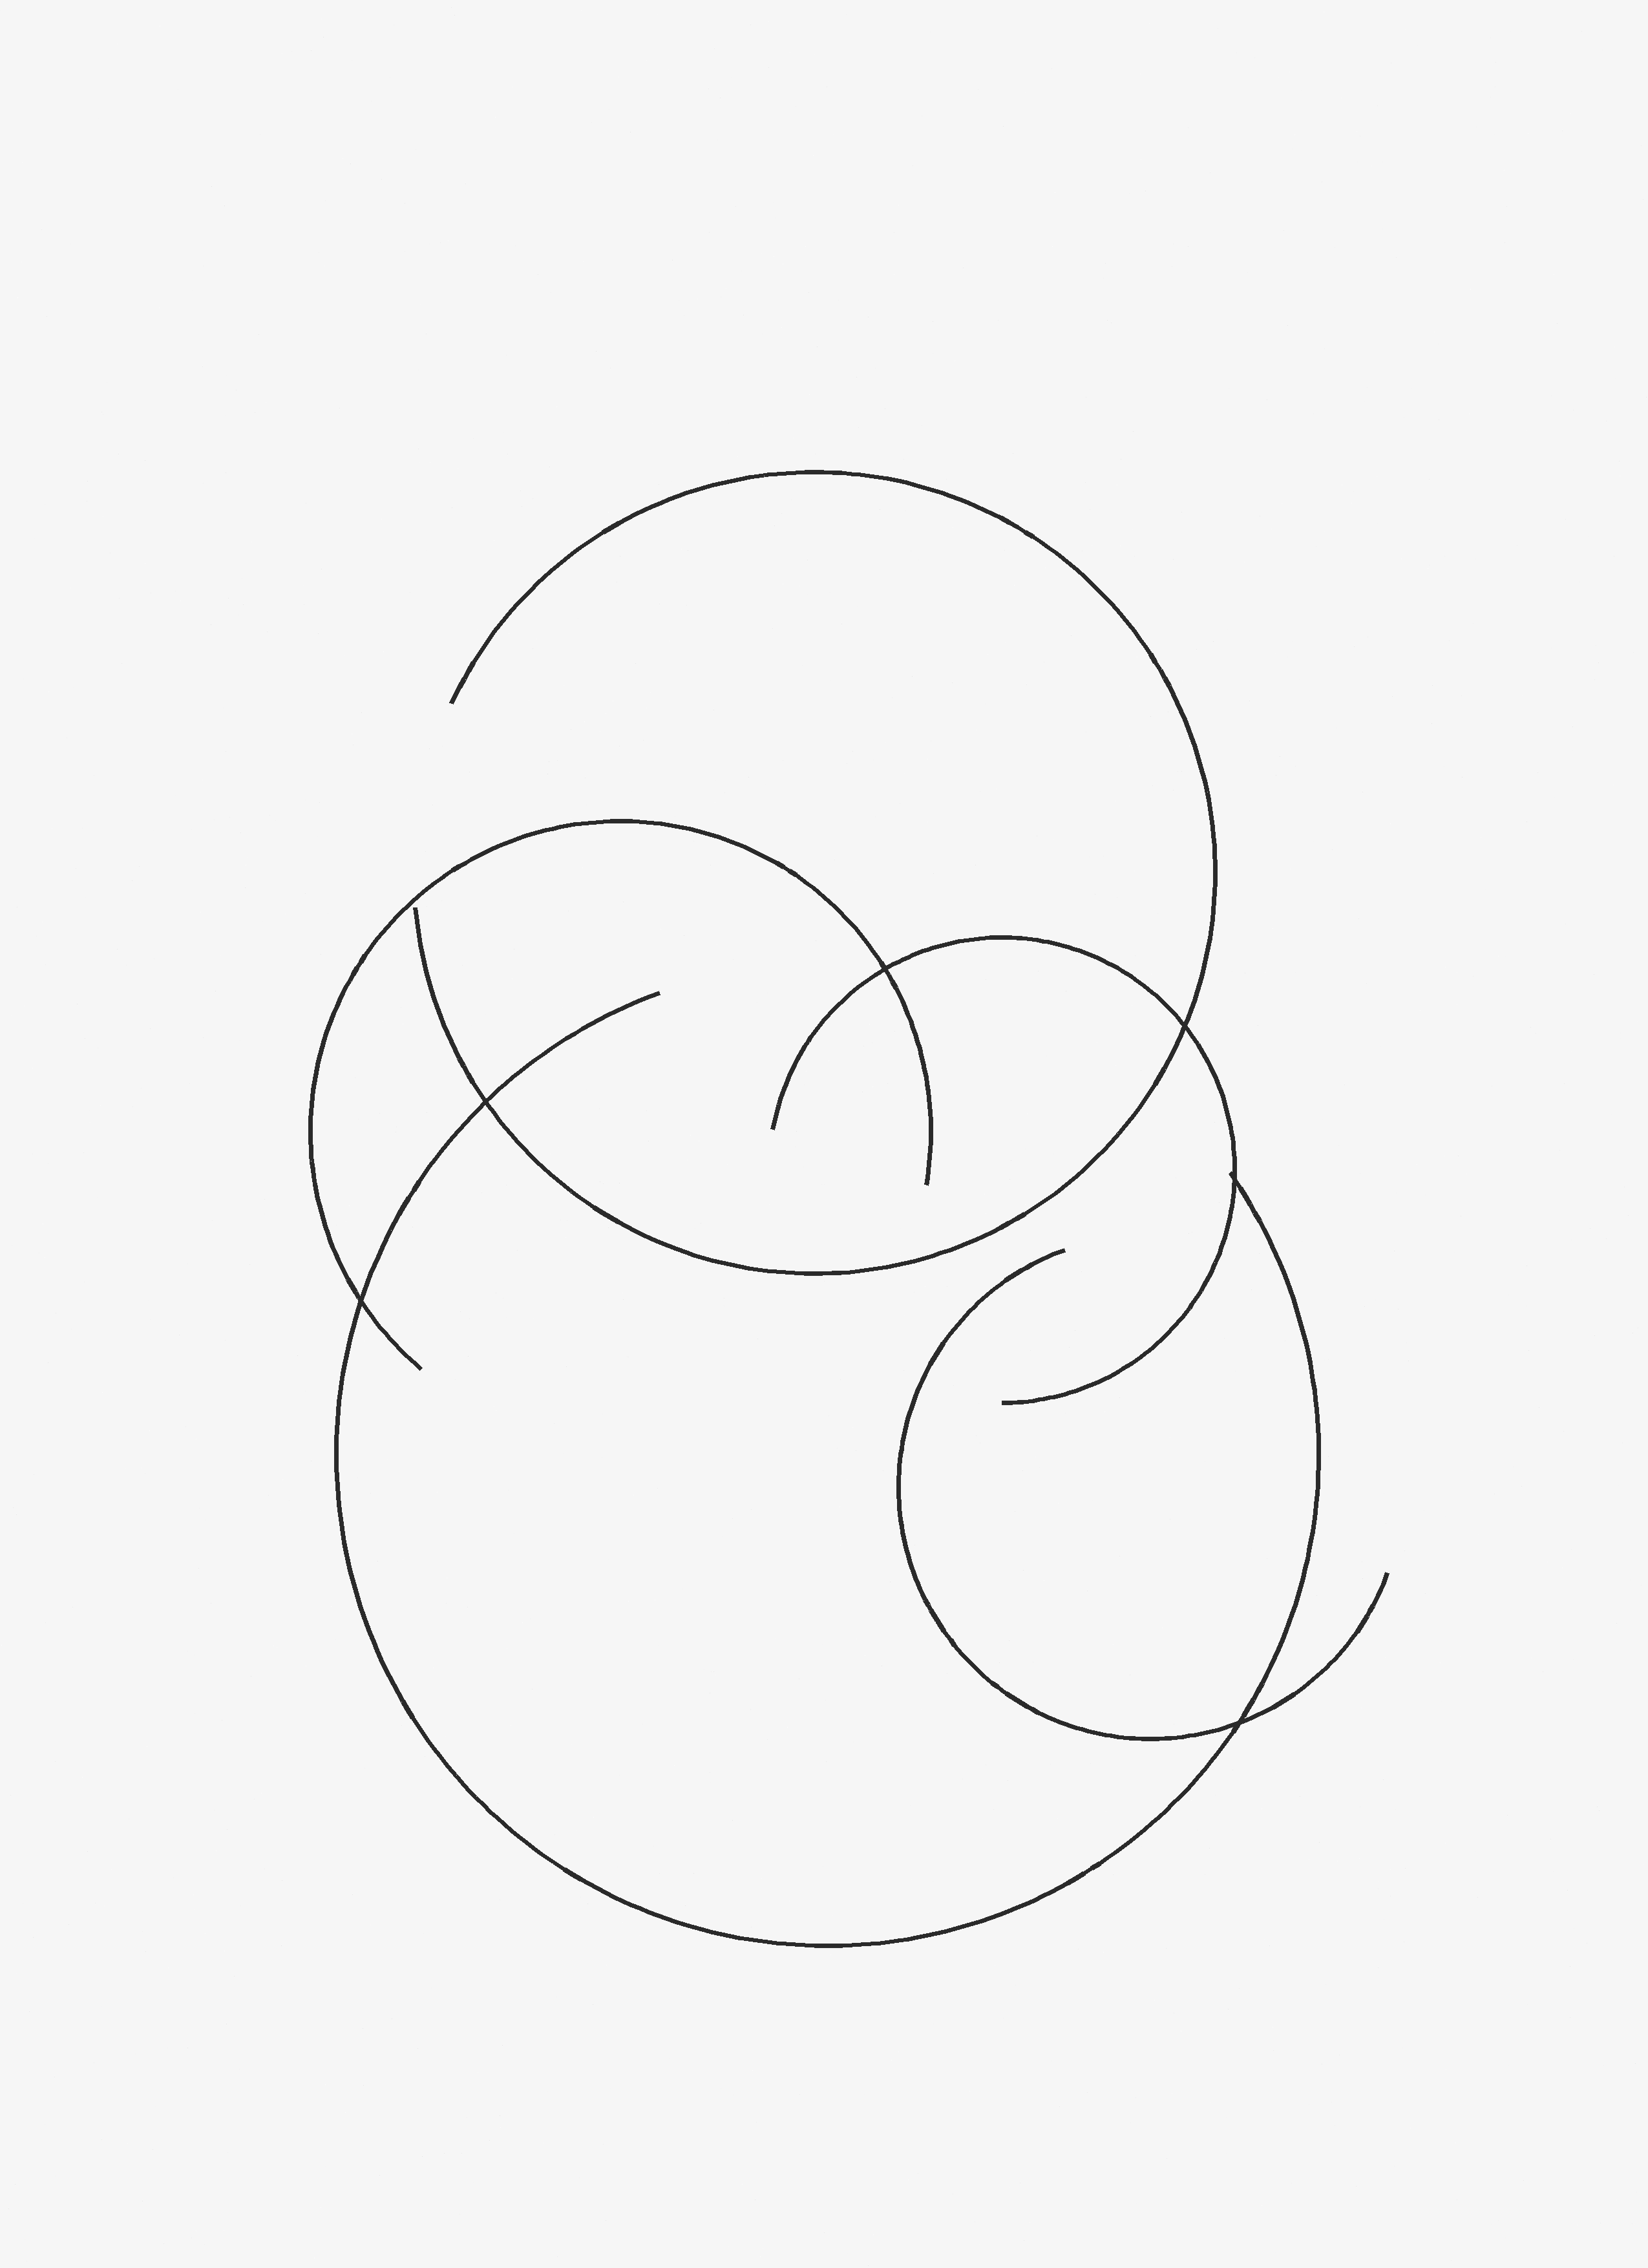
\includegraphics[width=\linewidth,height=0.42\textheight,keepaspectratio]{processamento/sintetica_020_cinza.png}
\end{minipage}
\hfill
\begin{minipage}{0.32\linewidth}
\centering
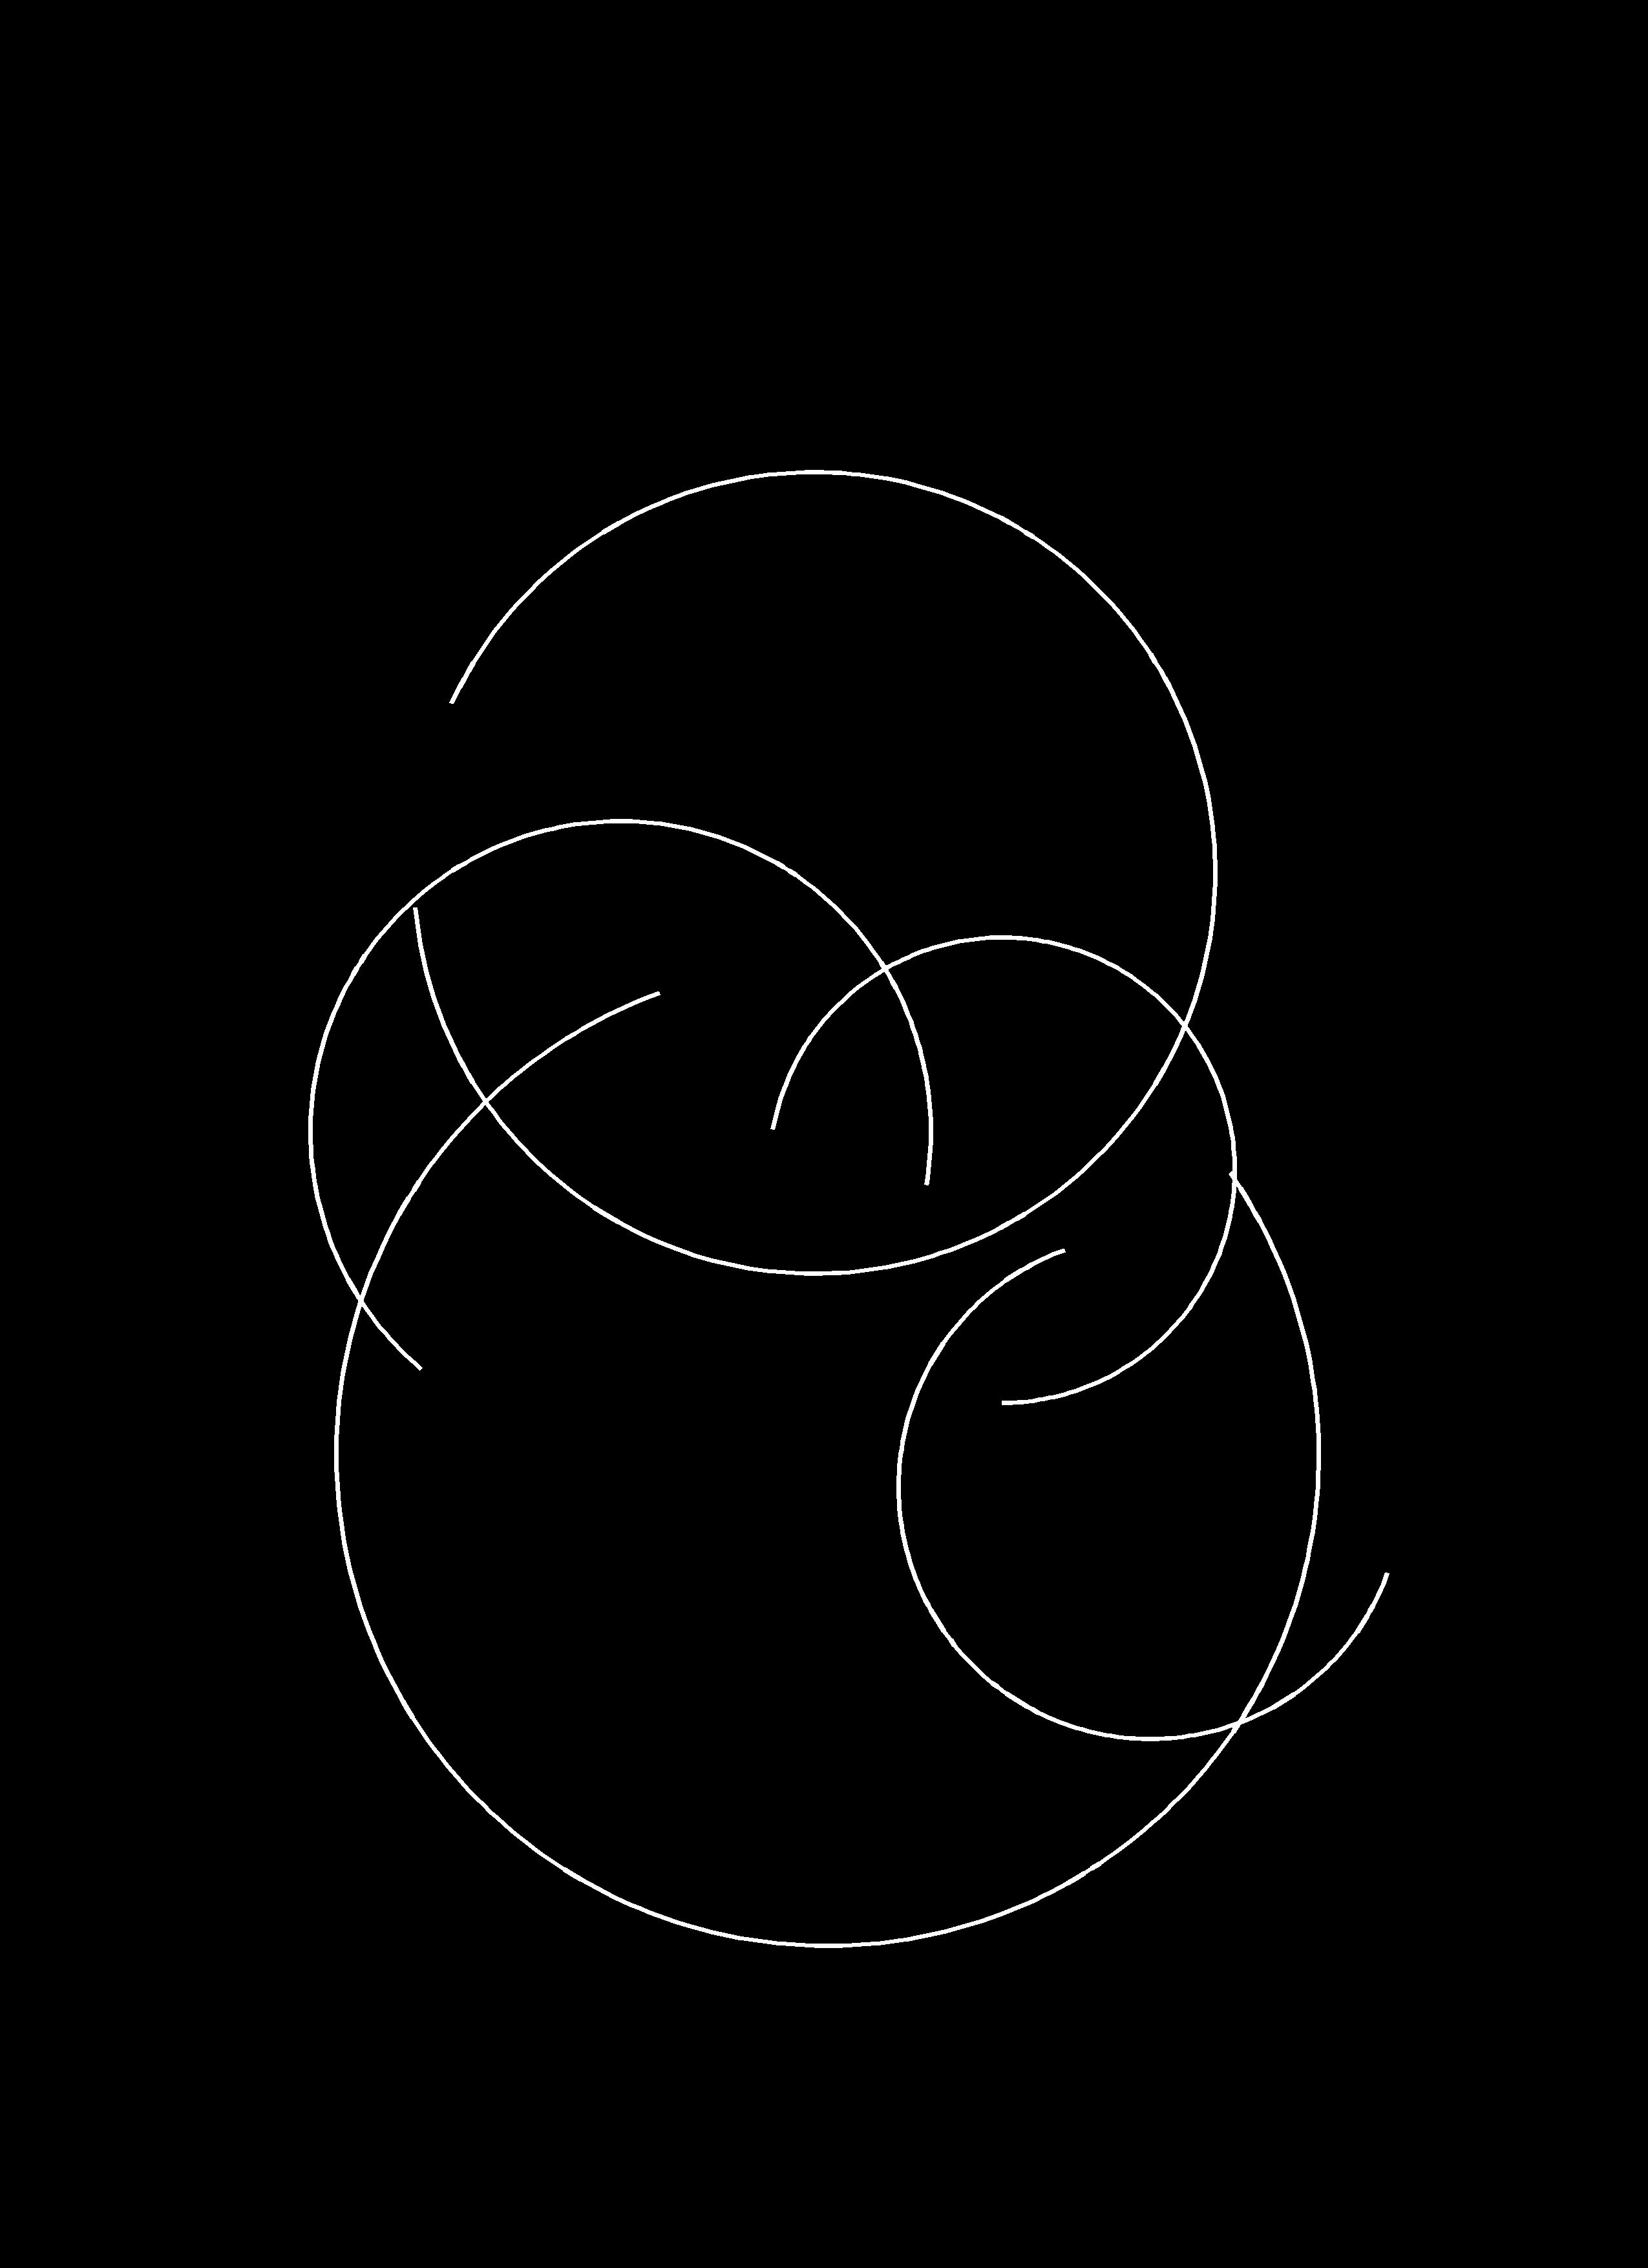
\includegraphics[width=\linewidth,height=0.42\textheight,keepaspectratio]{processamento/sintetica_020_segmentada.png}
\end{minipage}
\hfill
\begin{minipage}{0.32\linewidth}
\centering

\includegraphics[width=\linewidth,height=0.42\textheight,keepaspectratio]{processamento/sintetica_020_esqueleto.png}
\end{minipage}
\caption{Exemplo sintético: imagem em cinza, segmentação e esqueleto.}
\label{fig:proc-sintetica}
\end{figure}

\begin{figure}[!htbp]
\centering
\begin{minipage}{0.32\linewidth}
\centering
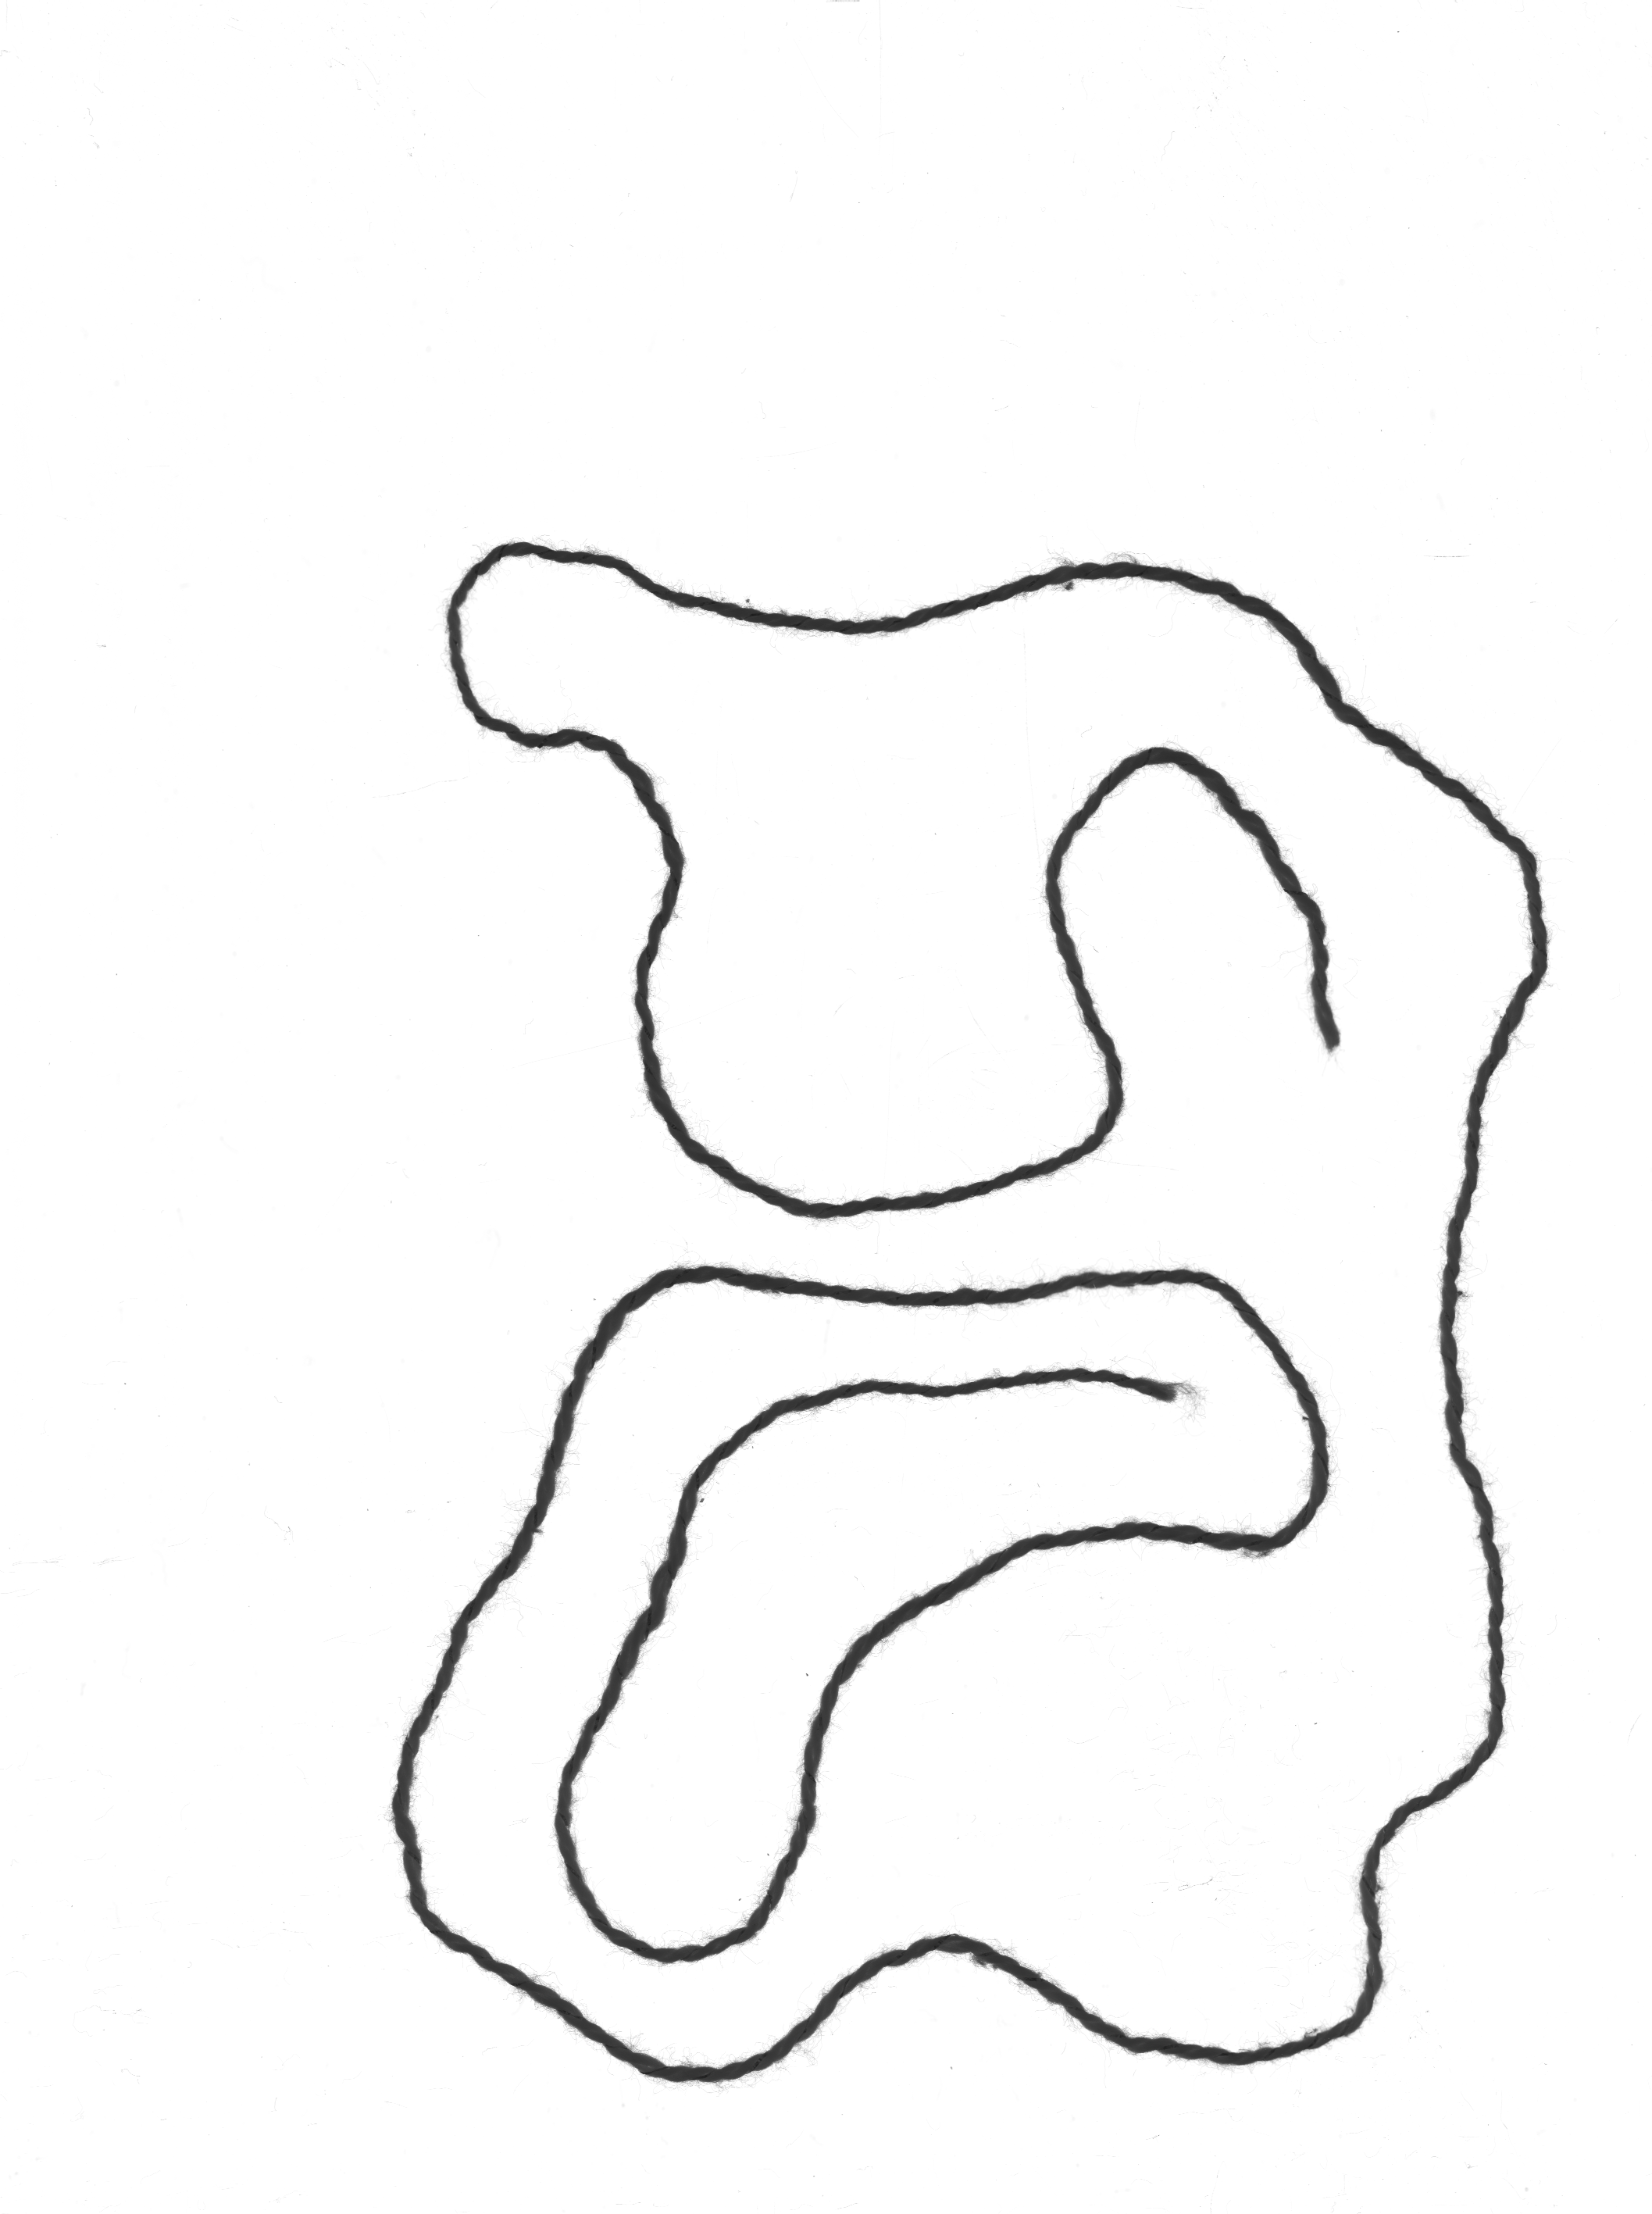
\includegraphics[width=\linewidth,height=0.42\textheight,keepaspectratio]{processamento/jean_1metro_cinza.png}
\end{minipage}
\hfill
\begin{minipage}{0.32\linewidth}
\centering
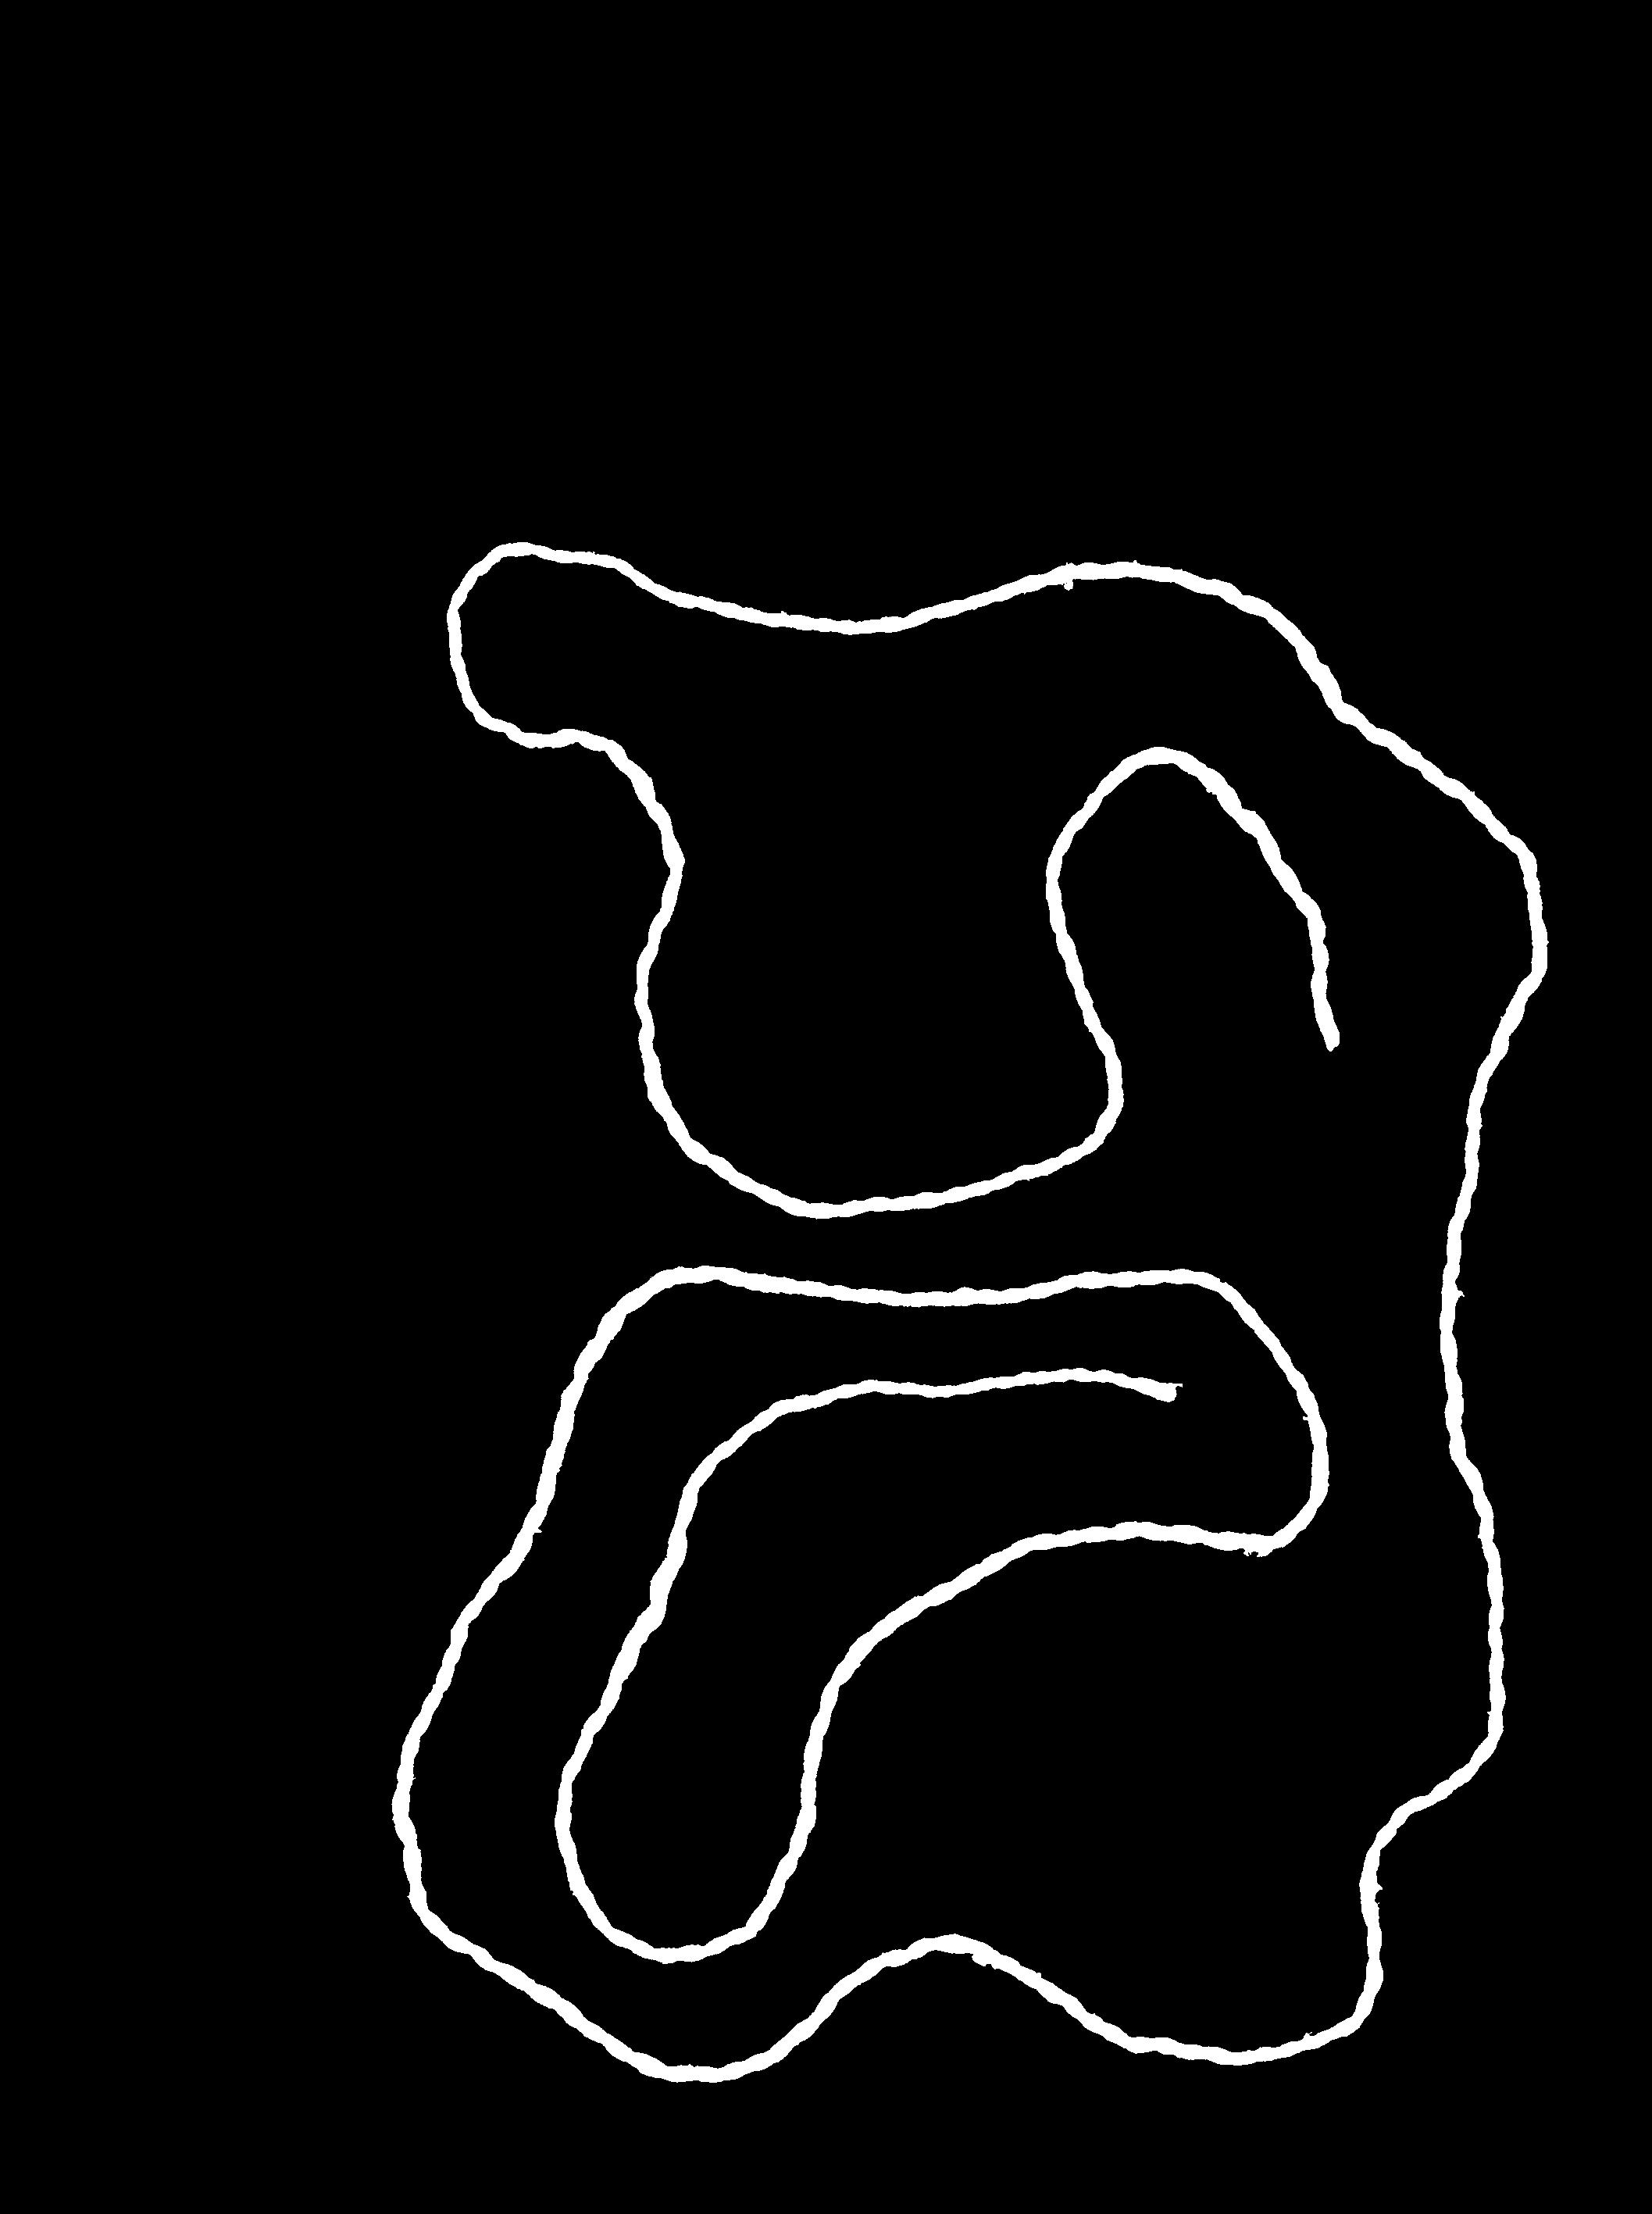
\includegraphics[width=\linewidth,height=0.42\textheight,keepaspectratio]{processamento/jean_1metro_segmentada.png}
\end{minipage}
\hfill
\begin{minipage}{0.32\linewidth}
\centering
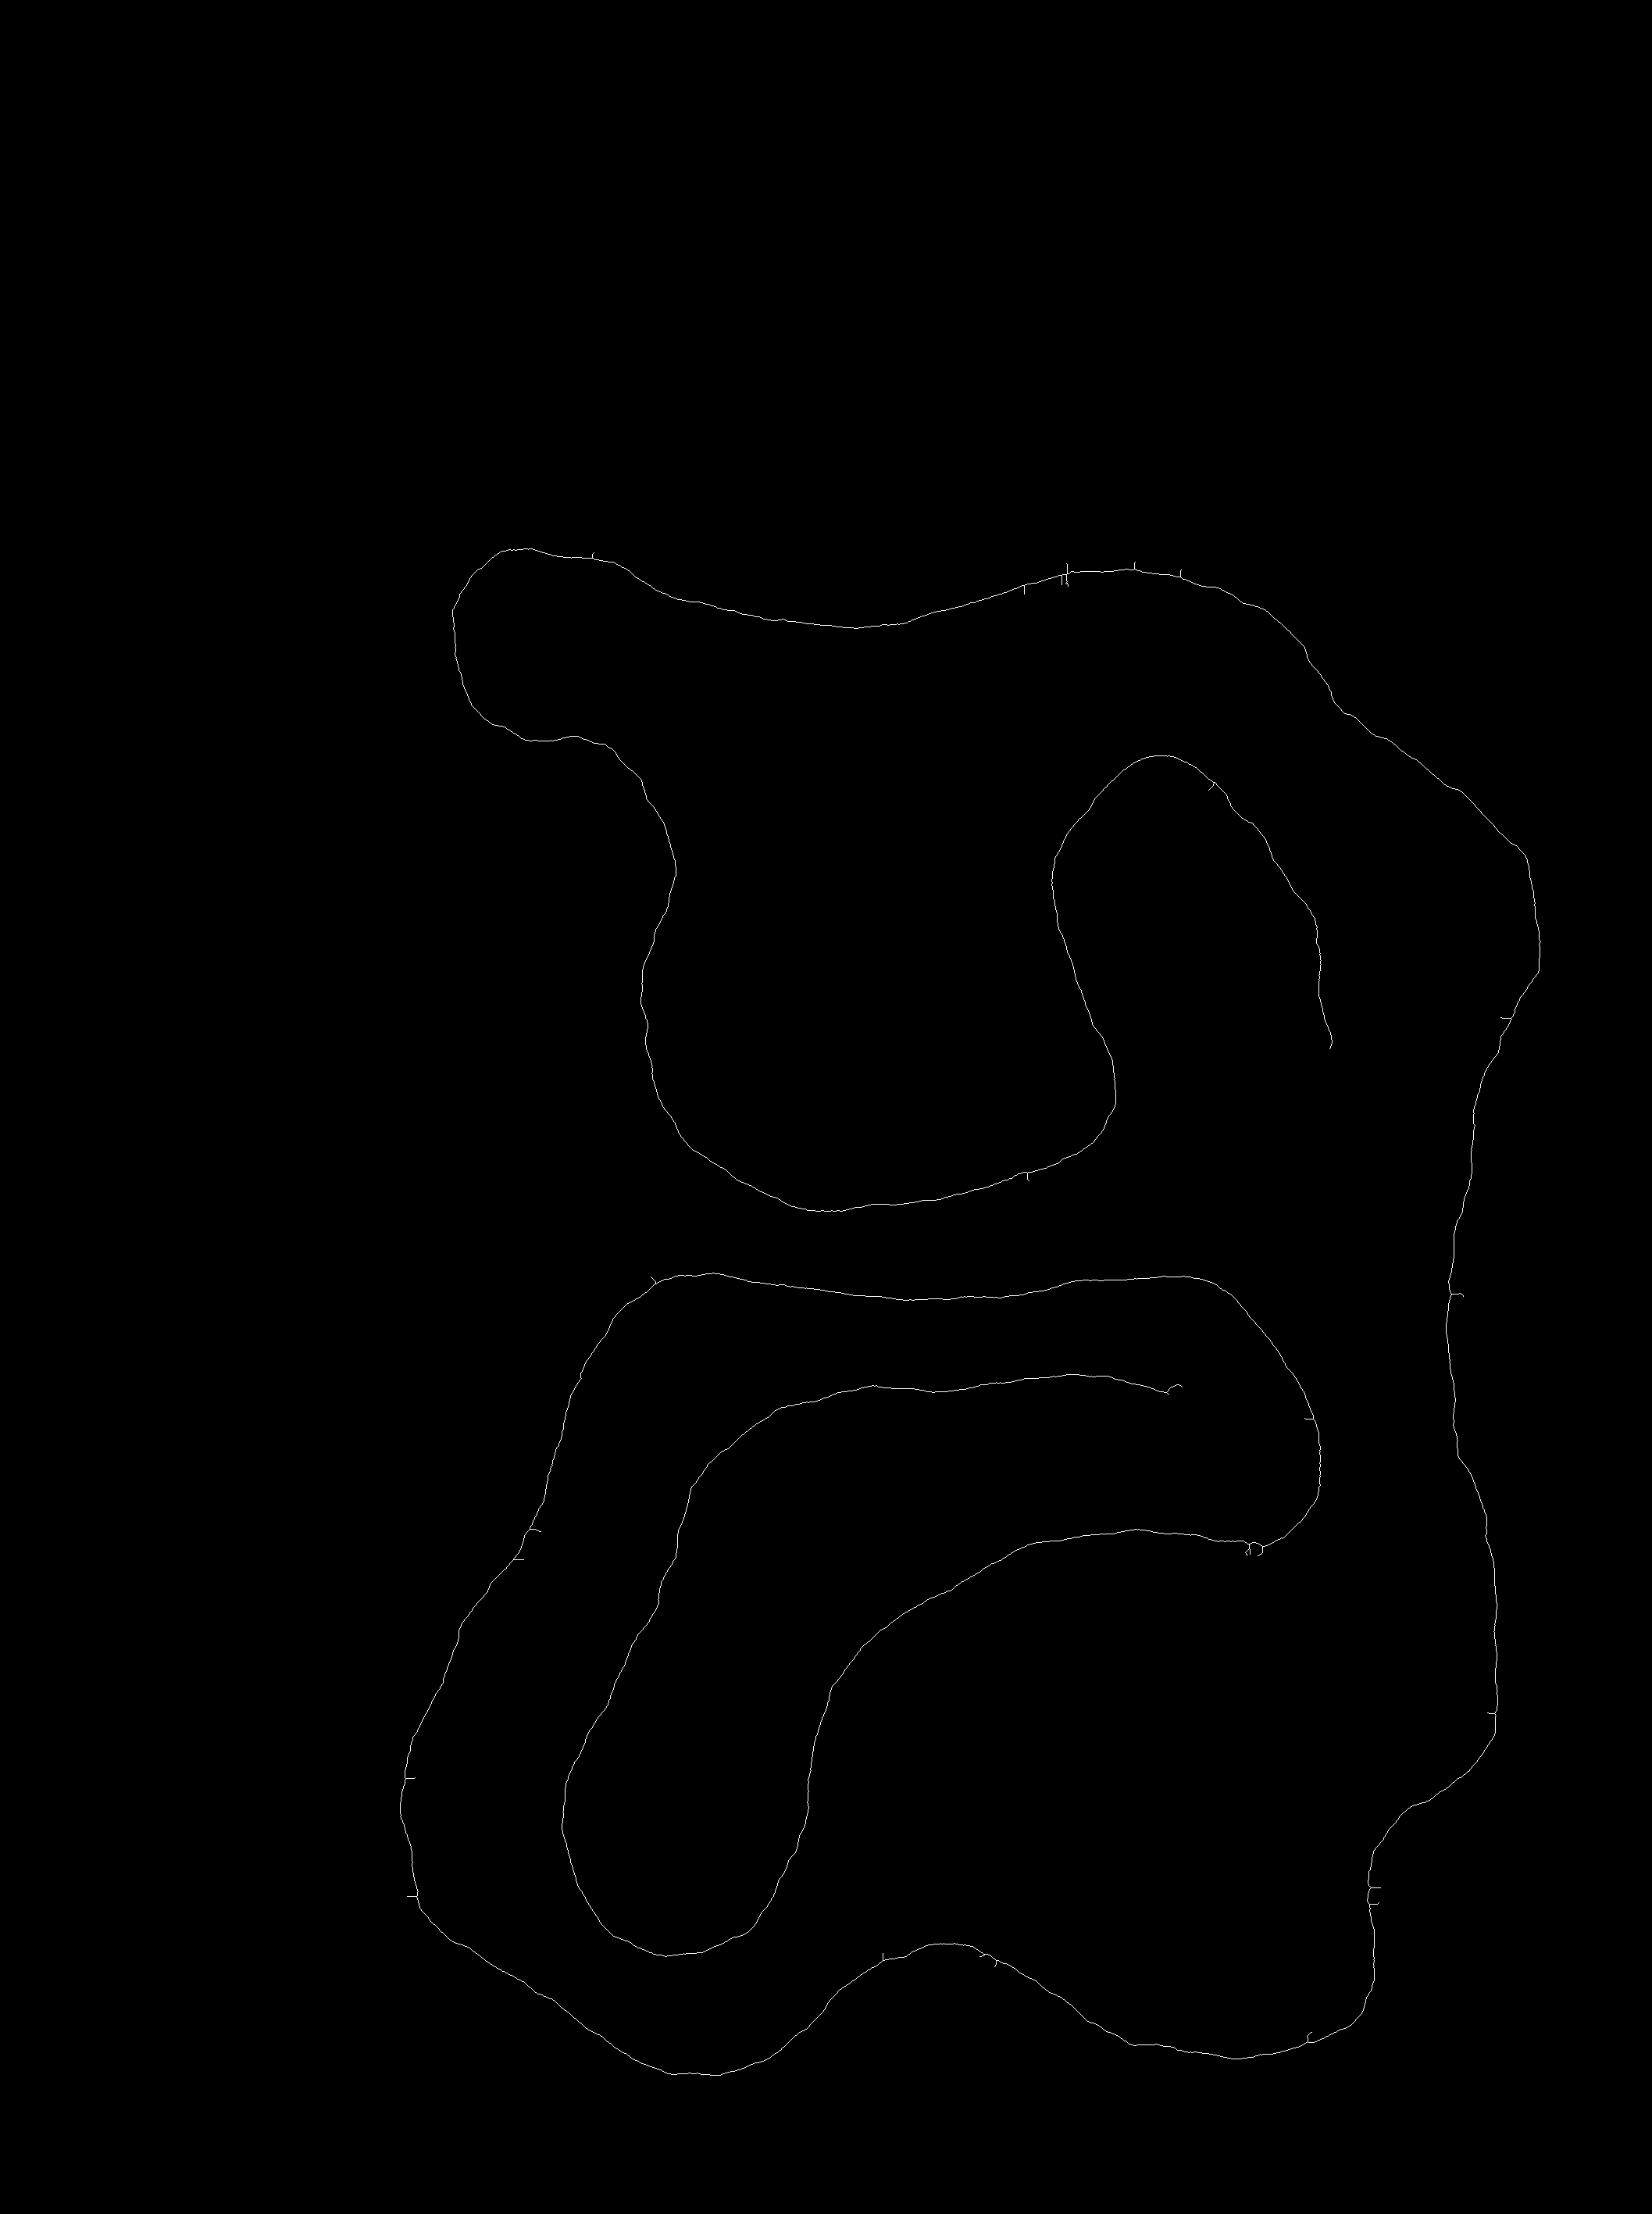
\includegraphics[width=\linewidth,height=0.42\textheight,keepaspectratio]{processamento/jean_1metro_esqueleto.png}
\end{minipage}
\caption{Exemplo Jean: imagem em cinza, segmentação e esqueleto.}
\label{fig:proc-jean}
\end{figure}

\begin{figure}[!htbp]
\centering
\begin{minipage}{0.32\linewidth}
\centering
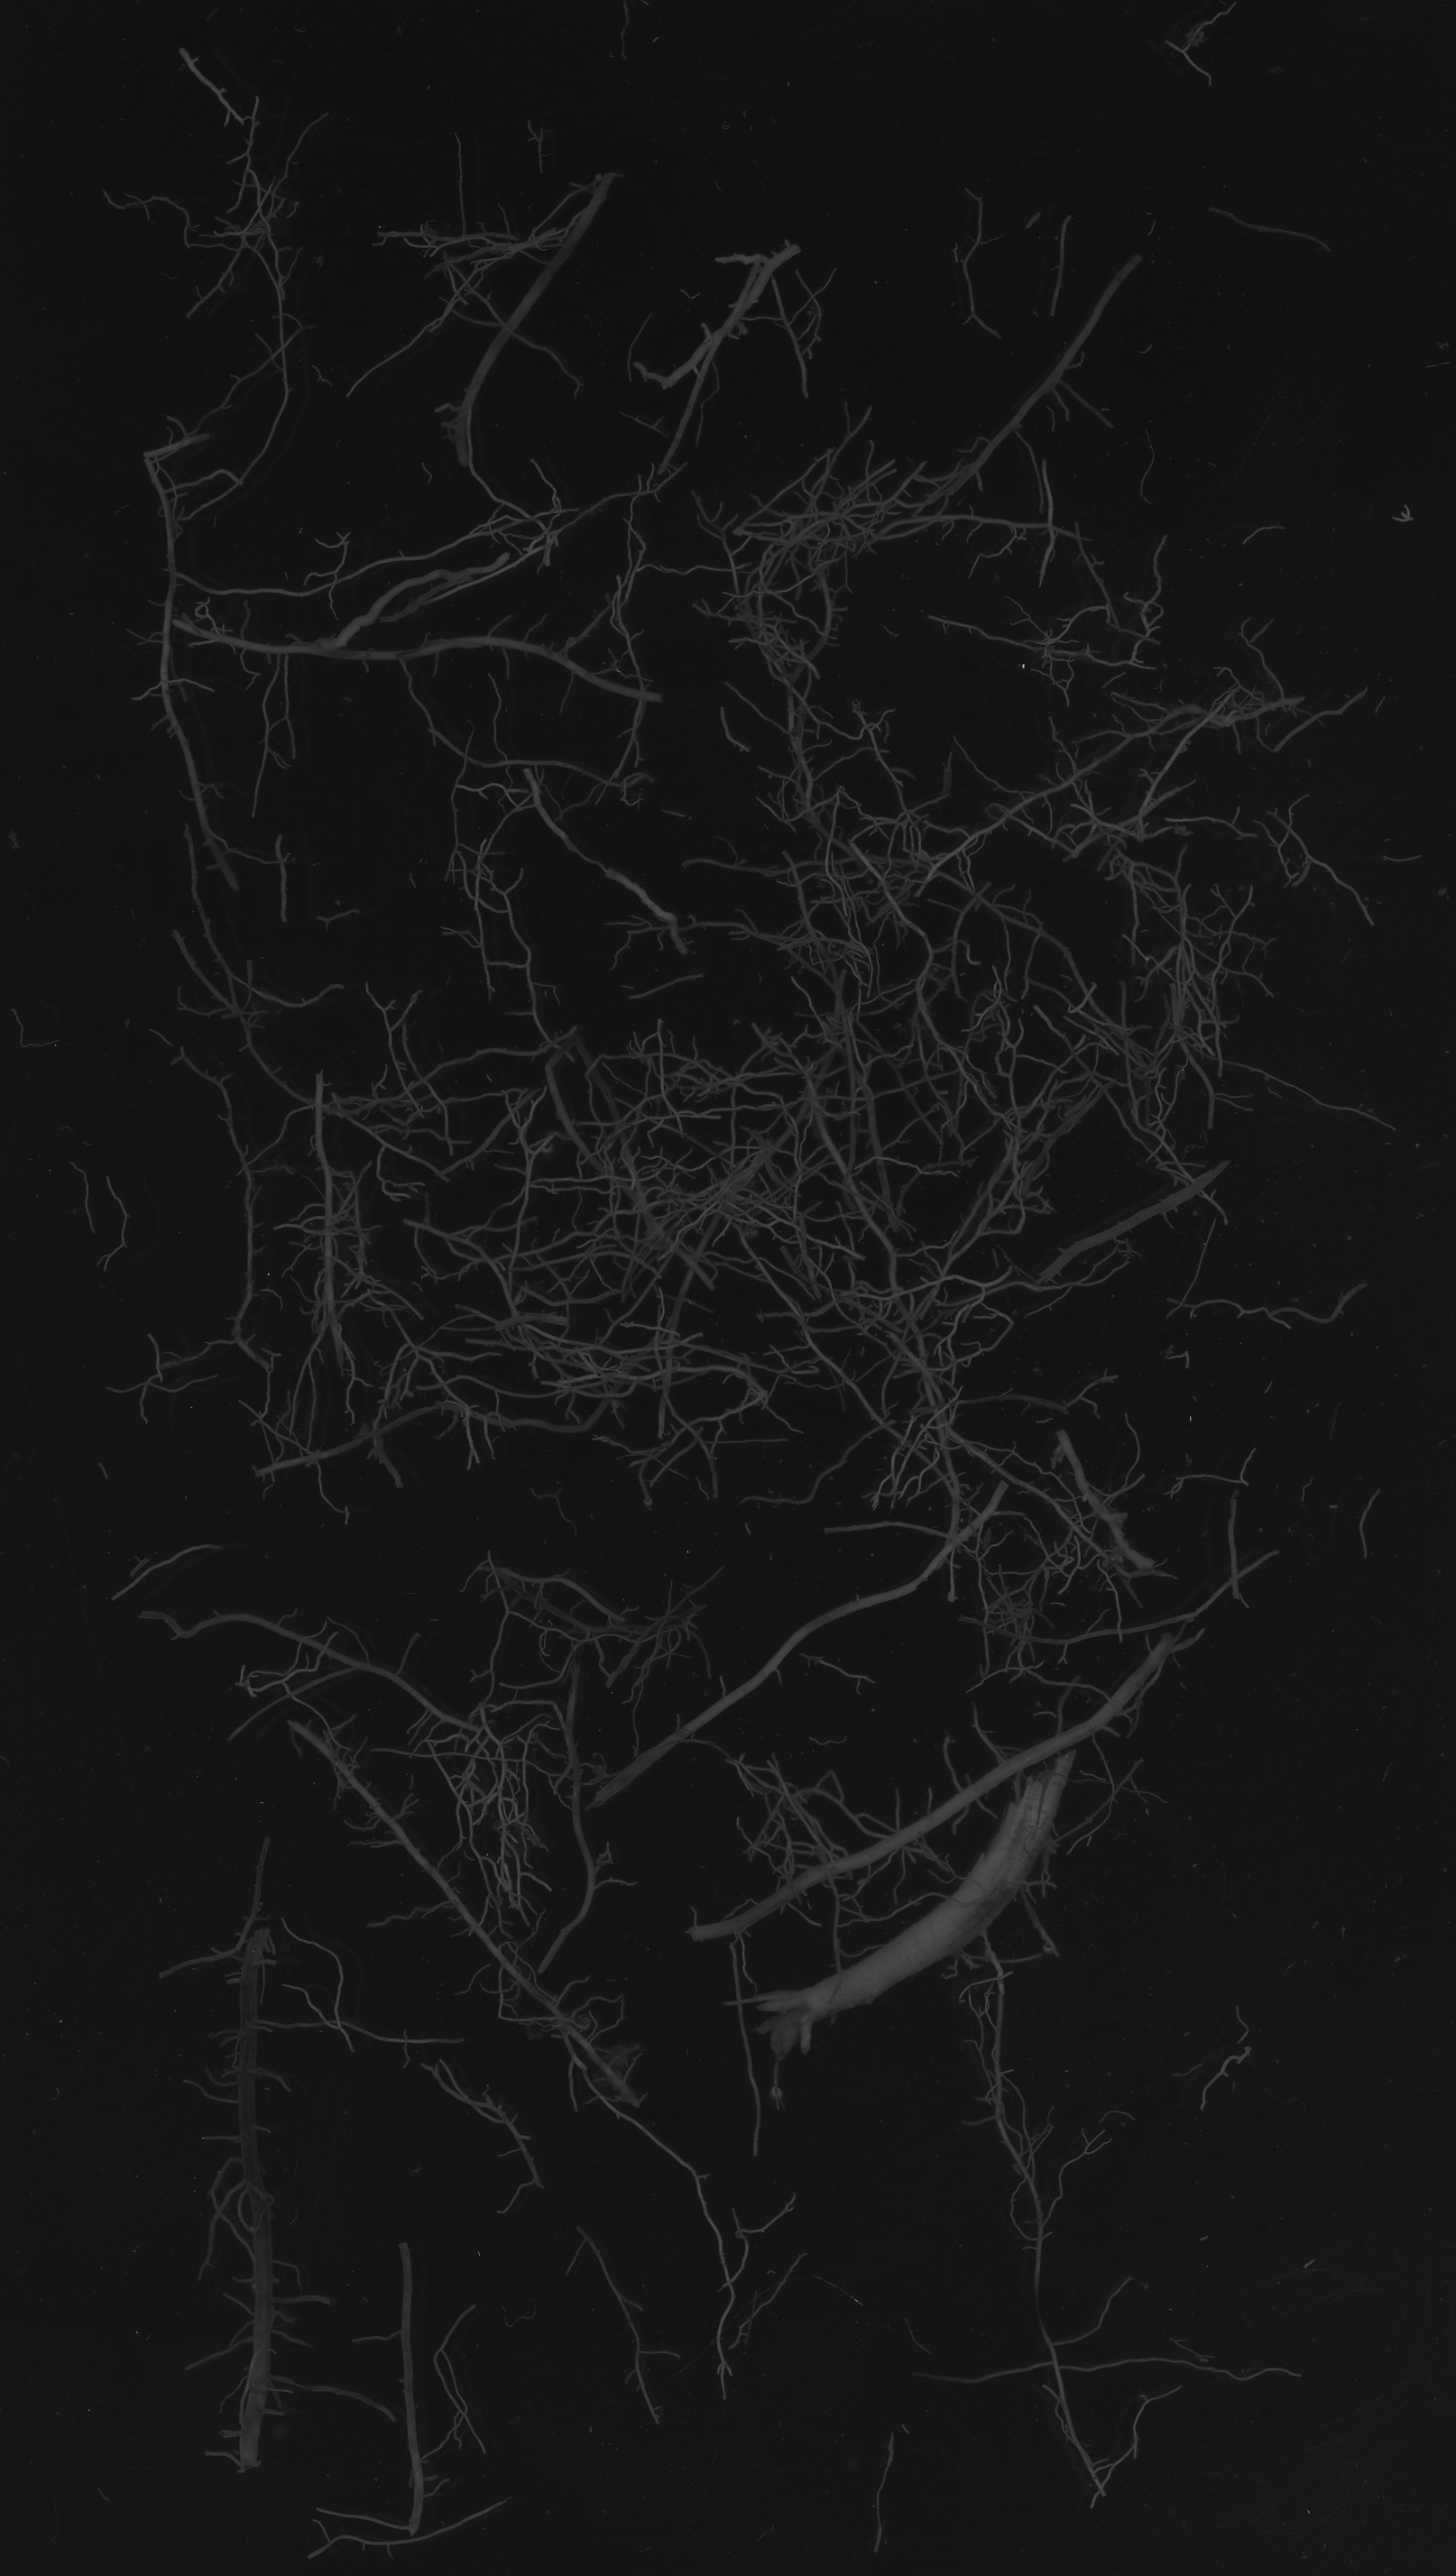
\includegraphics[width=\linewidth,height=0.42\textheight,keepaspectratio]{processamento/teruo_7487_cinza.png}
\end{minipage}
\hfill
\begin{minipage}{0.32\linewidth}
\centering
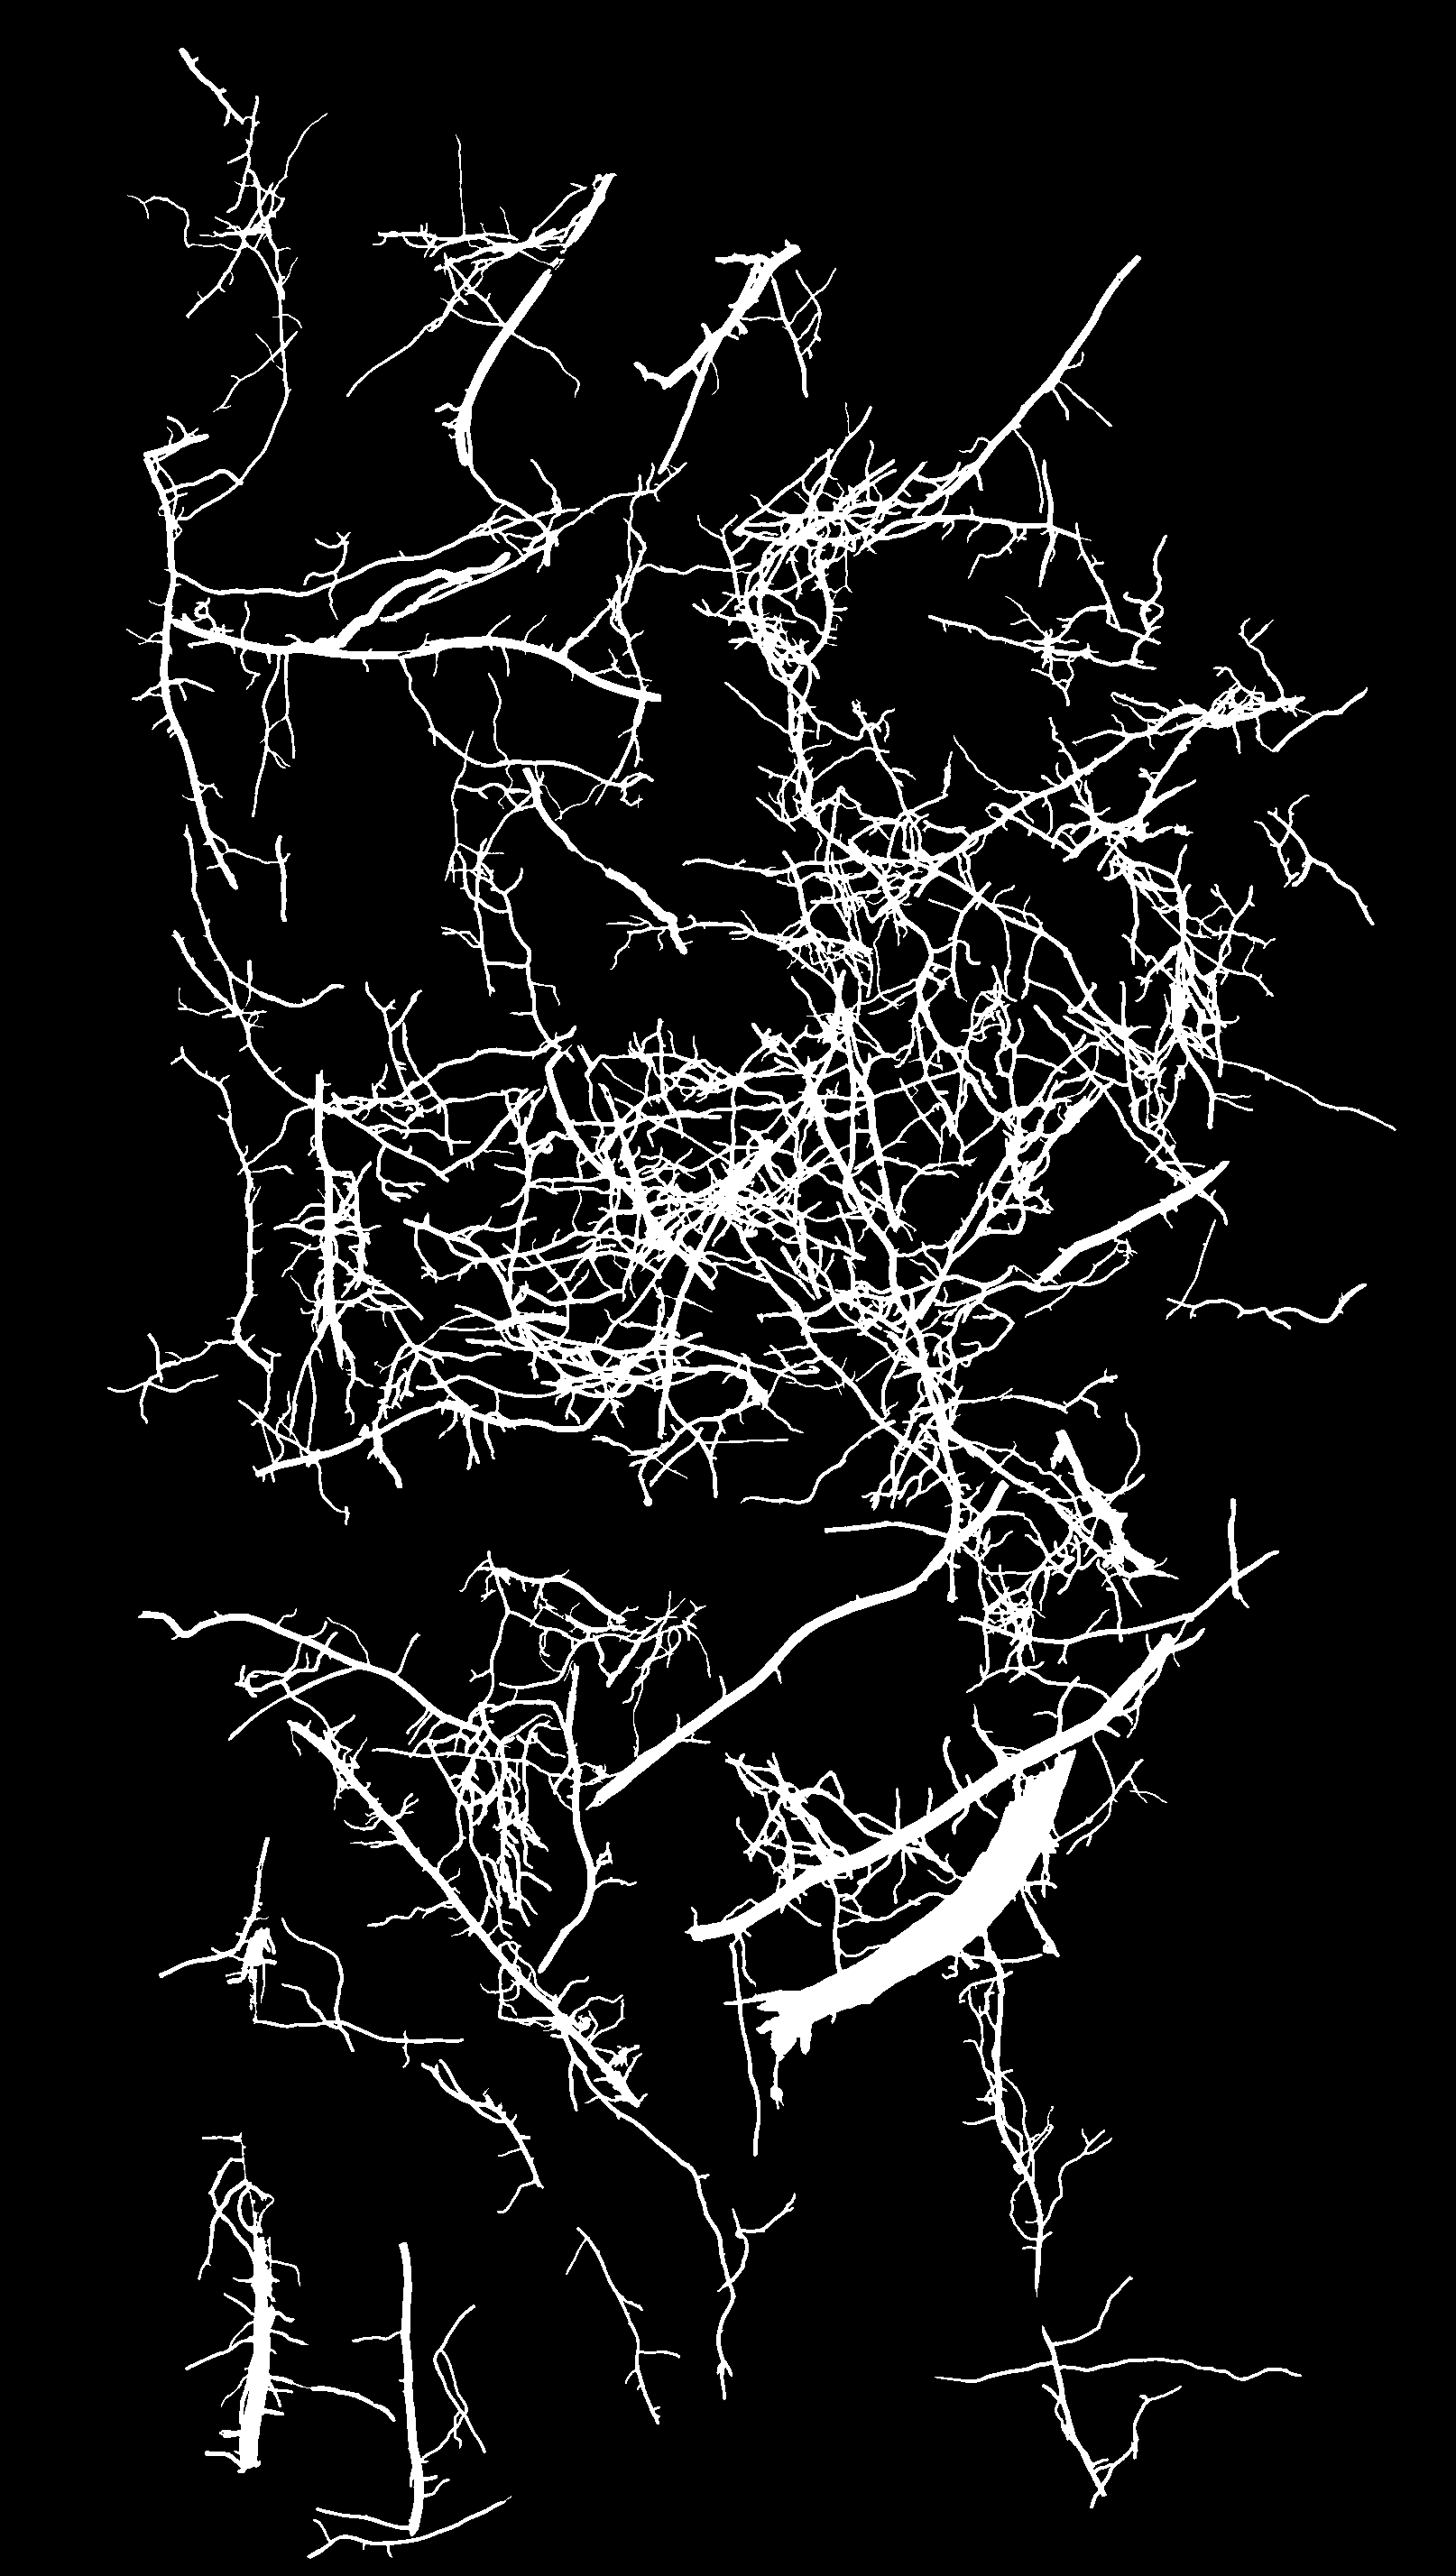
\includegraphics[width=\linewidth,height=0.42\textheight,keepaspectratio]{processamento/teruo_7487_segmentada.png}
\end{minipage}
\hfill
\begin{minipage}{0.32\linewidth}
\centering
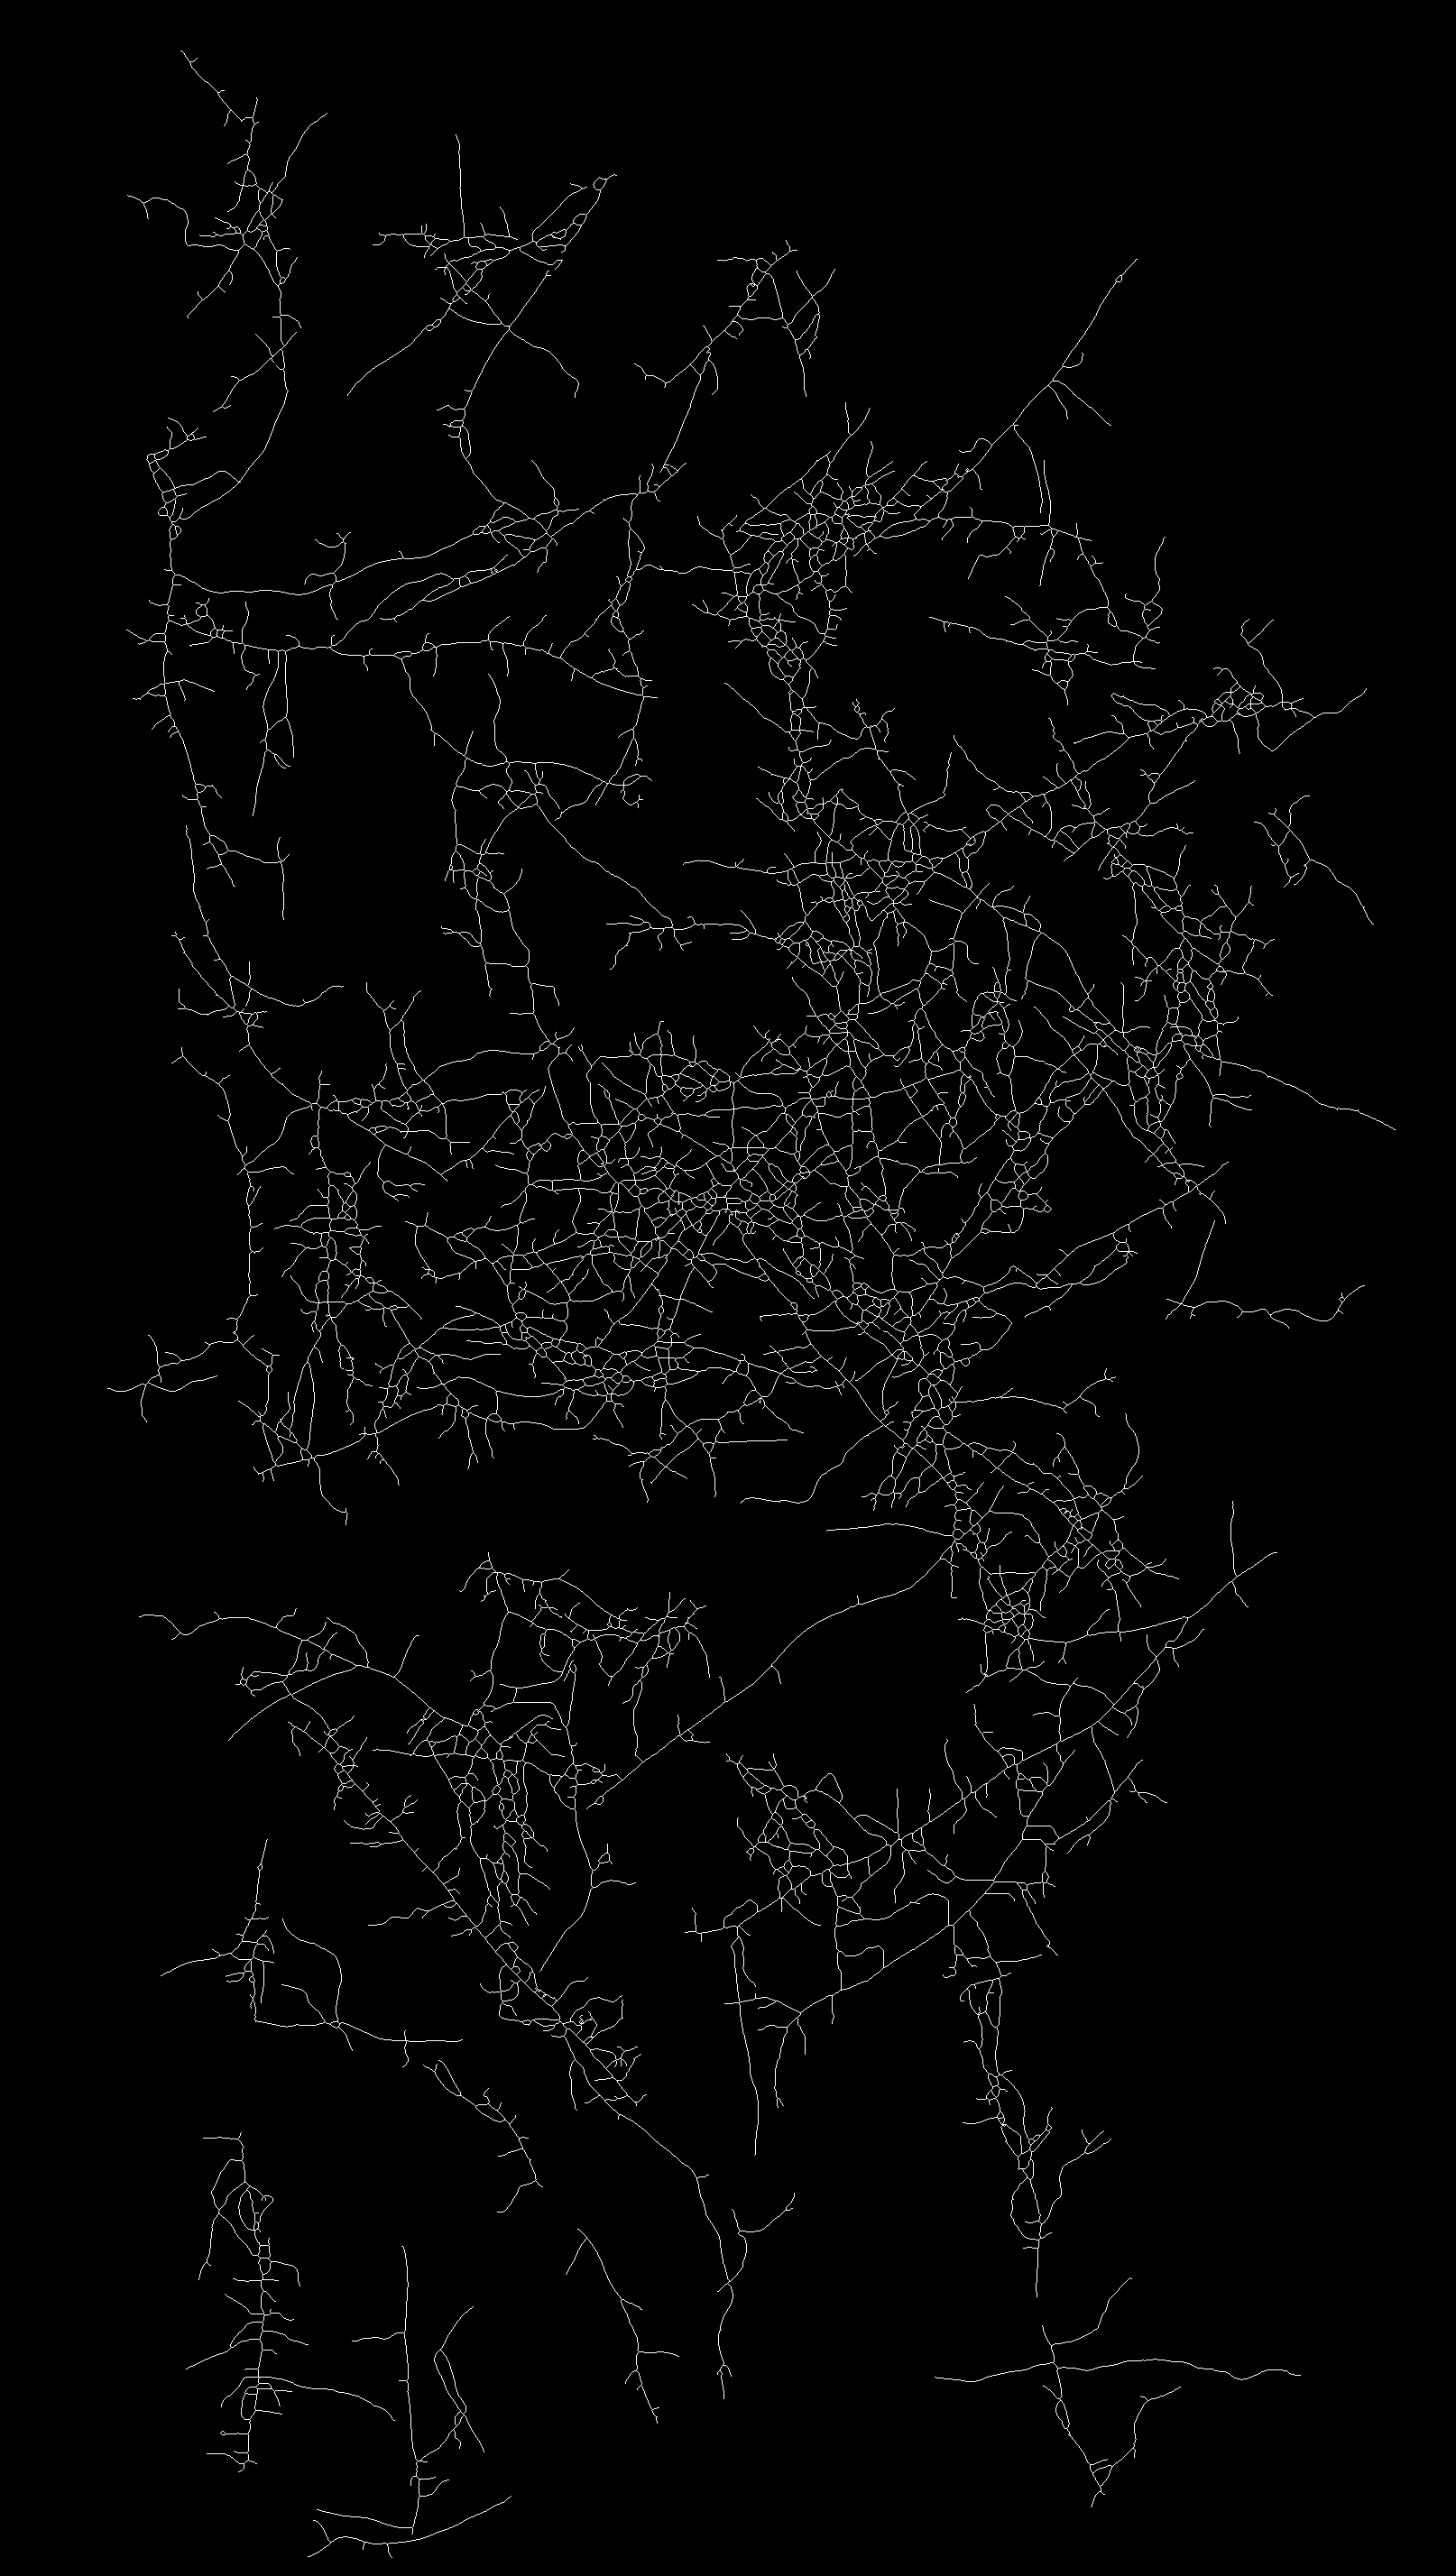
\includegraphics[width=\linewidth,height=0.42\textheight,keepaspectratio]{processamento/teruo_7487_esqueleto.png}
\end{minipage}
\caption{Exemplo Teruo: imagem em cinza, segmentação e esqueleto.}
\label{fig:proc-teruo}
\end{figure}

\subsection{Cálculo do comprimento}

O comprimento usa uma cadeia geométrica. Se dois pixels vizinhos do esqueleto estão lado a lado, o passo vale 1 pixel. Se estão em diagonal, o passo vale $\sqrt{2}$ pixels. Assim:

\[
L_{px} = N_{ortogonal} + \sqrt{2}\cdot N_{diagonal}.
\]

Nessa expressão, $L_{px}$ é o comprimento total do esqueleto medido em pixels; $N_{ortogonal}$ é a quantidade de ligações horizontais e verticais entre pixels vizinhos do esqueleto; e $N_{diagonal}$ é a quantidade de ligações na diagonal. O fator $\sqrt{2} \approx 1{,}414$ é o comprimento da diagonal de um pixel de lado unitário, obtido pelo teorema de Pitágoras. Cabe destacar que a contagem é de ligações entre pixels, e não de pixels: uma linha com $n$ pixels possui $n-1$ ligações.

O comprimento em milímetros é:

\[
L_{mm} = L_{px}\cdot pixelSize.
\]

Aqui, $L_{mm}$ é o comprimento em milímetros e $pixelSize$ é o tamanho físico do pixel, em milímetros, dado por $25,4/DPI$. A 300 DPI, por exemplo, $pixelSize = 0{,}0847$ mm.

O sistema calcula ainda, na mesma passagem, a área projetada, o diâmetro médio e o número de pontos de ramificação, todos exportados no CSV. Como essas grandezas não foram confrontadas com referência independente, elas não são objeto de análise neste artigo e são mencionadas apenas para registro: a área corresponde à contagem de pixels da máscara multiplicada por $pixelSize^2$; o diâmetro médio é obtido pelo dobro da distância até a borda, medida sobre os pixels do esqueleto pela transformada de distância; e os pontos de ramificação são os pixels do esqueleto com mais de dois vizinhos. A implementação de cada uma está disponível no código do projeto.

\subsection{Validação das medidas}
\label{sec:validacao}

A validação foi realizada com três grupos de imagens, resumidos na Tabela~\ref{tab:datasets}: sintéticas, scanner Jean e scanner Teruo. Todas as referências foram extraídas do nome do arquivo. Nas imagens de scanner Jean, nomes como \texttt{1,6Metro.bmp} foram convertidos para 1600 mm. Nas imagens de scanner Teruo, nomes como \texttt{37 - 3000.bmp} foram interpretados pelo valor após o hífen, ou seja, 3000 mm. Nas imagens sintéticas, o valor esperado foi lido do sufixo em milímetros.

Os dois conjuntos de scanner diferem quanto à natureza da amostra, e essa distinção é relevante para interpretar os resultados. O conjunto Jean não é composto por raízes, e sim por fios de náilon dispostos sobre o scanner, em duas condições: fio contínuo e fio picotado em segmentos. Trata-se, portanto, de um objeto de calibração, e não de material biológico. A escolha tem uma vantagem metodológica clara: o fio possui espessura uniforme, comprimento estável e nenhuma ambiguidade sobre onde a estrutura começa ou termina, o que torna a aferição manual mais confiável e isola o comportamento geométrico do algoritmo de variações próprias da amostra. Em contrapartida, o conjunto não reproduz a complexidade de um sistema radicular real, com raízes finas, sobreposições e diferenças de espessura, papel que cabe ao conjunto Teruo. O fio picotado, em particular, foi incluído para reproduzir de forma controlada a fragmentação que ocorre quando a segmentação perde trechos da estrutura.

É preciso deixar claro o que esses nomes representam nos dois conjuntos de scanner. Neles, o valor gravado no nome do arquivo é o comprimento aferido manualmente com trena, por um operador humano, antes da digitalização da amostra. Trata-se, portanto, de uma medida de referência e não de um valor exato. A medição manual de estruturas finas, curvas e ramificadas com instrumento graduado em milímetros está sujeita a erro de leitura, a erro de posicionamento da trena ao acompanhar trechos curvos, ao achatamento ou estiramento da amostra durante o manuseio e à variação entre operadores. É razoável supor que a incerteza dessa aferição seja de ordem milimétrica ou superior, e que ela cresça com o comprimento total da amostra, já que trechos longos exigem reposicionamentos sucessivos do instrumento.

Ainda assim, essa é a referência mais confiável disponível para o propósito deste trabalho. Ela é independente do software avaliado, foi obtida antes e fora do processo de digitalização, não depende de nenhum parâmetro do \textit{pipeline} e está registrada de forma verificável no próprio nome do arquivo, o que mantém o experimento reproduzível. A alternativa seria adotar a saída de outro software de análise de imagem como referência, o que apenas transferiria o problema, pois passaria a comparar dois métodos computacionais entre si em vez de comparar o sistema com uma medida física. Por esse motivo, os erros percentuais relatados adiante devem ser entendidos como divergência entre a medida automática e a medida manual, e não como erro absoluto do sistema em relação ao comprimento verdadeiro da raiz. Essa ressalva é particularmente relevante nas amostras curtas, nas quais um desvio de poucos milímetros na aferição manual já representa parcela expressiva do erro percentual.

O conjunto sintético foi construído precisamente para contornar essa limitação. Nos dois conjuntos de scanner, qualquer divergência observada é a soma de duas parcelas indistinguíveis: o erro do algoritmo e o erro da aferição manual com trena. Não há como separá-las, porque não existe uma terceira medida independente. Ao gerar imagens por computador, com o traçado definido antes da imagem, elimina-se por completo a parcela humana: o valor de referência deixa de ser uma medição e passa a ser um dado de projeto, exato por construção. O erro medido nesse conjunto é, portanto, atribuível apenas ao método, o que torna a conclusão sobre o comportamento do algoritmo mais firme do que seria possível apenas com amostras físicas.

Essa separação também permite atribuir causa aos desvios. Como cada imagem sintética foi desenhada para representar uma situação geométrica específica — reta, curva contínua, cruzamentos, fragmentação, baixo contraste, estruturas finas ou espessas —, um erro elevado em determinado caso aponta diretamente qual característica da imagem o algoritmo não trata bem, sem a ambiguidade que uma amostra real introduziria.

O programa gerador está disponível no repositório do projeto, no arquivo \texttt{Testes/Sintéticas/gerar\_imagens\_sinteticas.py}, junto da tabela \texttt{comprimentos\_esperados.csv}, que registra para cada imagem o comprimento esperado, o DPI, as dimensões, o tipo de fundo e a espessura utilizada. Isso permite que qualquer pessoa regenere as vinte imagens e confira os valores de referência de forma independente.

No caso das imagens sintéticas, o valor de referência não foi estimado a partir da imagem, mas definido antes dela. Cada figura foi construída a partir de uma descrição geométrica prévia, composta por segmentos de reta, arcos e curvas com comprimento analítico conhecido em milímetros. Esse comprimento é a soma dos comprimentos das primitivas usadas no desenho e foi escrito no sufixo do nome do arquivo; a soma dos vinte arquivos resulta nos 61214 mm do grupo sintético. As primitivas foram então rasterizadas em 300 DPI, com espessura controlada, o que fixa a relação entre milímetro e pixel. A IA generativa foi utilizada apenas para propor a aparência e a variedade morfológica dos casos de teste (reta, curva, rede densa, cruzamentos, fragmentos, baixo contraste), enquanto o comprimento de referência veio sempre da definição geométrica que originou o traçado, e não de medição posterior sobre a imagem. Assim, a topologia gerada não precisa reproduzir fielmente uma raiz biológica: o papel do conjunto sintético é isolar o comportamento do algoritmo diante de situações geométricas conhecidas, com \textit{ground truth} exato, deixando para os conjuntos de scanner a avaliação em condições reais.

Reforça-se o escopo desta validação: apenas o comprimento total foi confrontado com valor de referência, pois as imagens utilizadas não possuem valores nominais para as demais grandezas. Todos os resultados apresentados a seguir referem-se, portanto, exclusivamente ao comprimento.

Todos os testes usaram a mesma rotina do \textit{backend}, com limiar automático, suavização ativada, filtragem de componentes ativada, poda de esqueleto ativada e DPI manual de 300. Nenhuma imagem recebeu limiar manual, recorte ou ajuste individual de parâmetro: as três opções avançadas foram mantidas ligadas para todo o conjunto, de modo que a comparação entre grupos reflita o mesmo procedimento.

Para permitir reprodução, os valores efetivos desses ajustes são os seguintes. A suavização é uma filtragem gaussiana com núcleo $3 \times 3$. A filtragem de componentes descarta objetos com área menor que $\max(36;\ 0{,}025\%\ \text{do total de pixels})$, em conectividade 8. A poda remove ramos terminais de até 0,25 mm e só é executada quando o esqueleto possui mais de 500 pixels, com no máximo seis iterações. Os resultados foram gravados em \texttt{resultados\_final.csv}, e as estatísticas em \texttt{estatisticas\_final.csv}.

Além dessas etapas, o \textit{backend} aplica duas correções heurísticas sobre o comprimento já calculado, e é necessário explicitá-las porque elas alteram o valor final. A primeira, identificada como \texttt{dense-graph}, atua quando a densidade de pontos de ramificação por milímetro ultrapassa um limite, situação típica de esqueletos que formaram malha por excesso de segmentação; nesse caso o comprimento é reduzido por um fator proporcional ao excesso de densidade. A segunda, identificada como \texttt{fragmented-components}, atua quando a máscara ficou muito fragmentada após a filtragem, e substitui o comprimento do esqueleto por uma estimativa derivada da razão entre área e diâmetro médio. O CSV registra, para cada imagem, o comprimento antes da correção, na coluna \texttt{raw\_length\_mm}, o valor final e qual correção foi acionada.

\vspace{5mm}

\begin{table}[!htbp]
\centering
\caption{Conjuntos usados na validação final.}
\label{tab:datasets}
\begin{tabular}{lrrp{6.8cm}}
\toprule
Grupo & n & Referência total (mm) & Característica principal \\
\midrule
Sintéticas & 20 & 61214 & Imagens geradas com comprimento conhecido no nome do arquivo. \\
Imagens Jean & 8 & 5315 & Fios de náilon digitalizados em duas condições, contínuo e picotado, com referência aferida por trena. \\
Imagens Teruo & 8 & 31985 & Raízes digitalizadas em scanner, com referência aferida por trena, em milímetros, no nome do arquivo. \\
Total & 36 & 98514 & Soma dos três grupos comparativos. \\
\bottomrule
\end{tabular}
\end{table}

As métricas calculadas foram erro percentual assinado, erro absoluto percentual, erro absoluto médio (MAE), raiz do erro quadrático médio (RMSE), mediana do erro absoluto, percentil 95 do erro absoluto e contagem de imagens dentro das tolerâncias de 3\%, 5\% e 10\%.

\section{Resultados e Discussões}

\subsection{Sistema desenvolvido}

Nesta seção são apresentados os resultados obtidos tanto com relação ao sistema desenvolvido quanto aos resultados de medidas obtidos. A sequência de processamento descrita na Seção~\ref{sec:etapas} foi implementada integralmente, e as telas a seguir mostram como cada etapa foi disponibilizada ao usuário.

\subsubsection{Seleção de arquivos}

As Figuras \ref{fig:ui-selecao-claro}, \ref{fig:ui-selecao-escuro}, e \ref{fig:ui-lista-lote} são as imagens da interface para seleção de arquivo, com o uso de modo claro e escuro, e quando da seleção de mais uma imagem para fins de análise em lote, respectivamente. A interface é intuitiva, dado que há somente uma possibilidade de ação, que é a de seleção de arquivo(s).

\begin{figure}[!htbp]
\centering
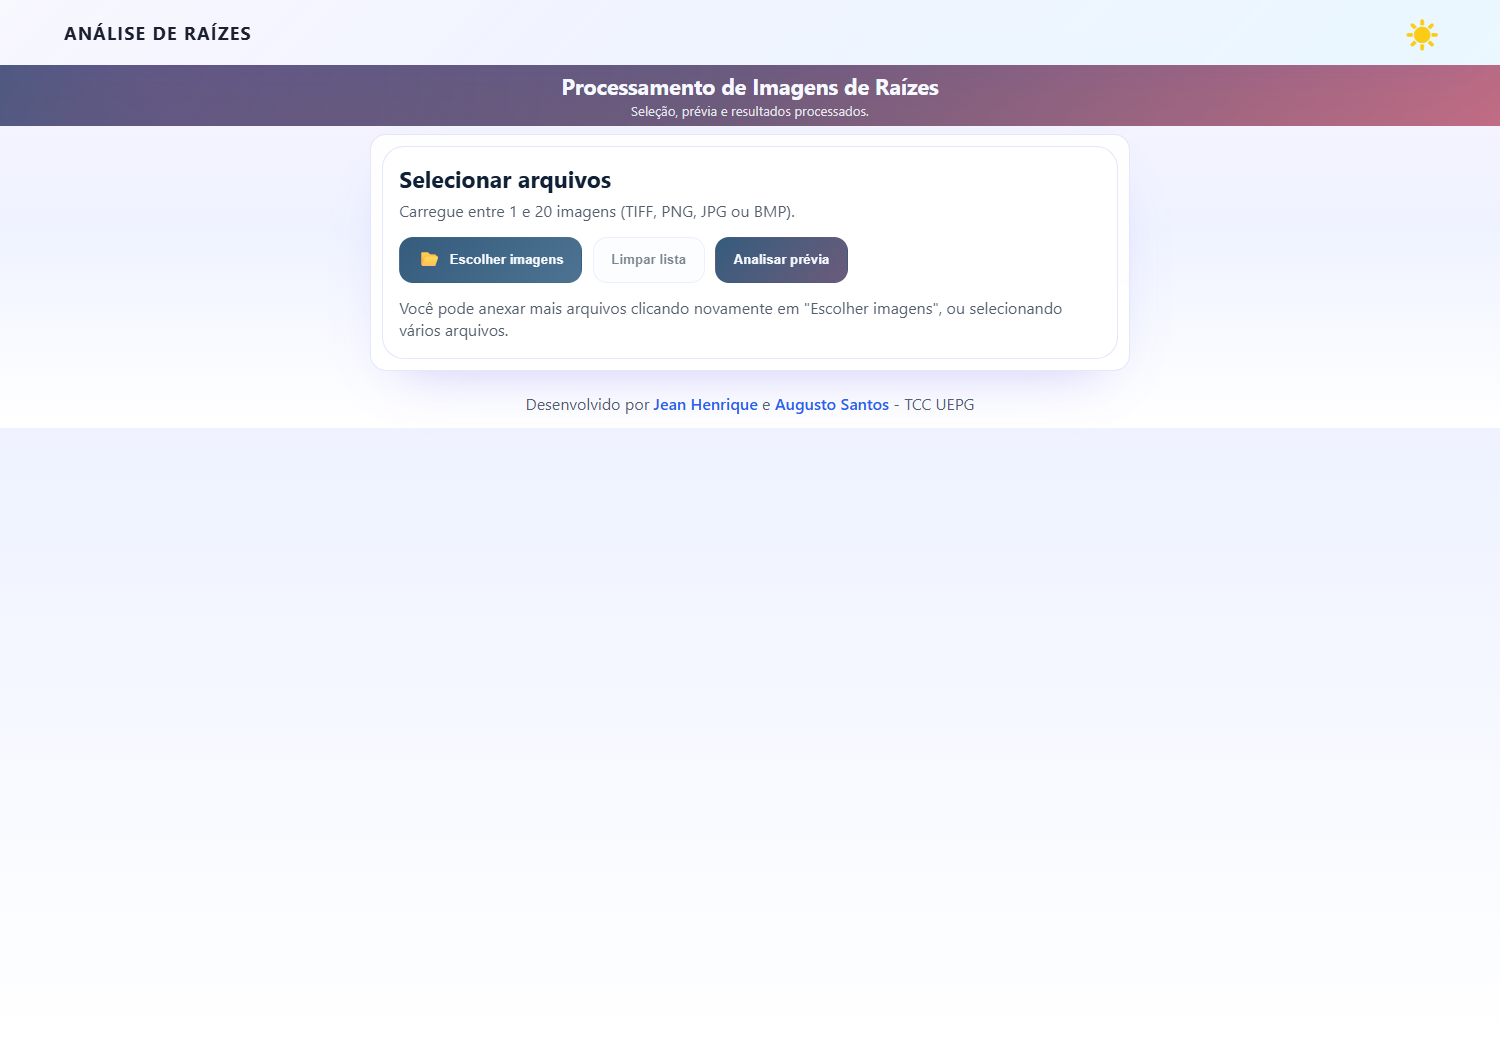
\includegraphics[width=\textwidth,height=0.58\textheight,keepaspectratio]{interface/tela_01_selecao_claro.png}
\caption{Tela inicial de seleção de imagens em tema claro.}
\label{fig:ui-selecao-claro}
\end{figure}

\begin{figure}[!htbp]
\centering
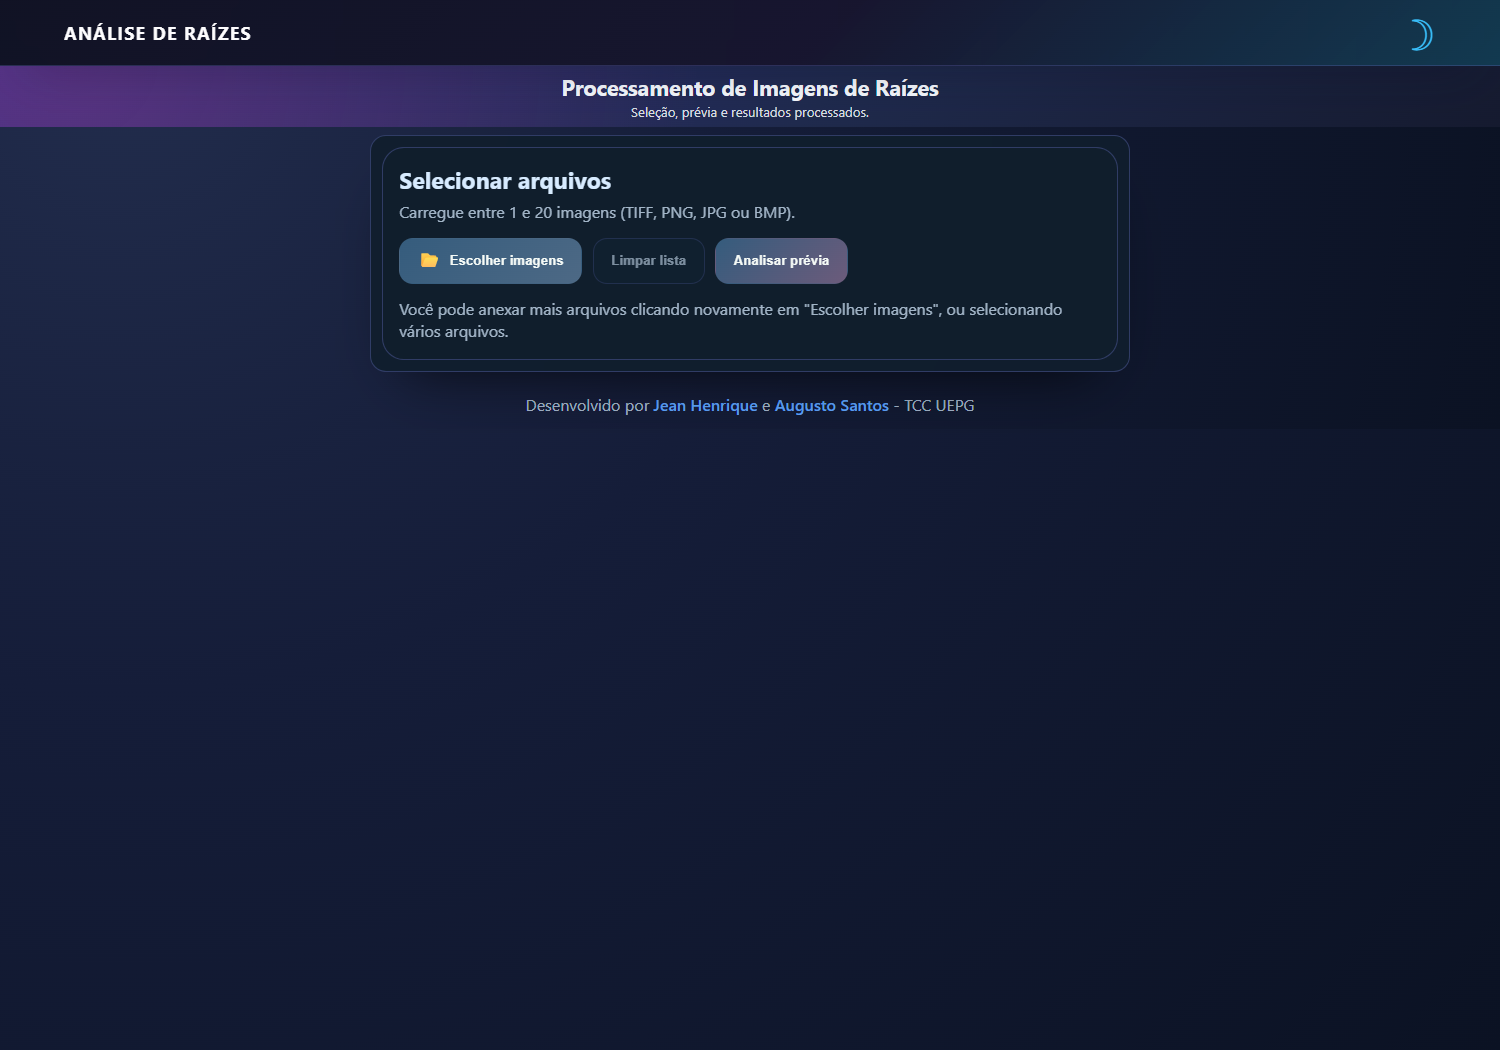
\includegraphics[width=\textwidth,height=0.58\textheight,keepaspectratio]{interface/tela_02_selecao_escuro.png}
\caption{Tela inicial de seleção de imagens em tema escuro.}
\label{fig:ui-selecao-escuro}
\end{figure}

\begin{figure}[!htbp]
\centering
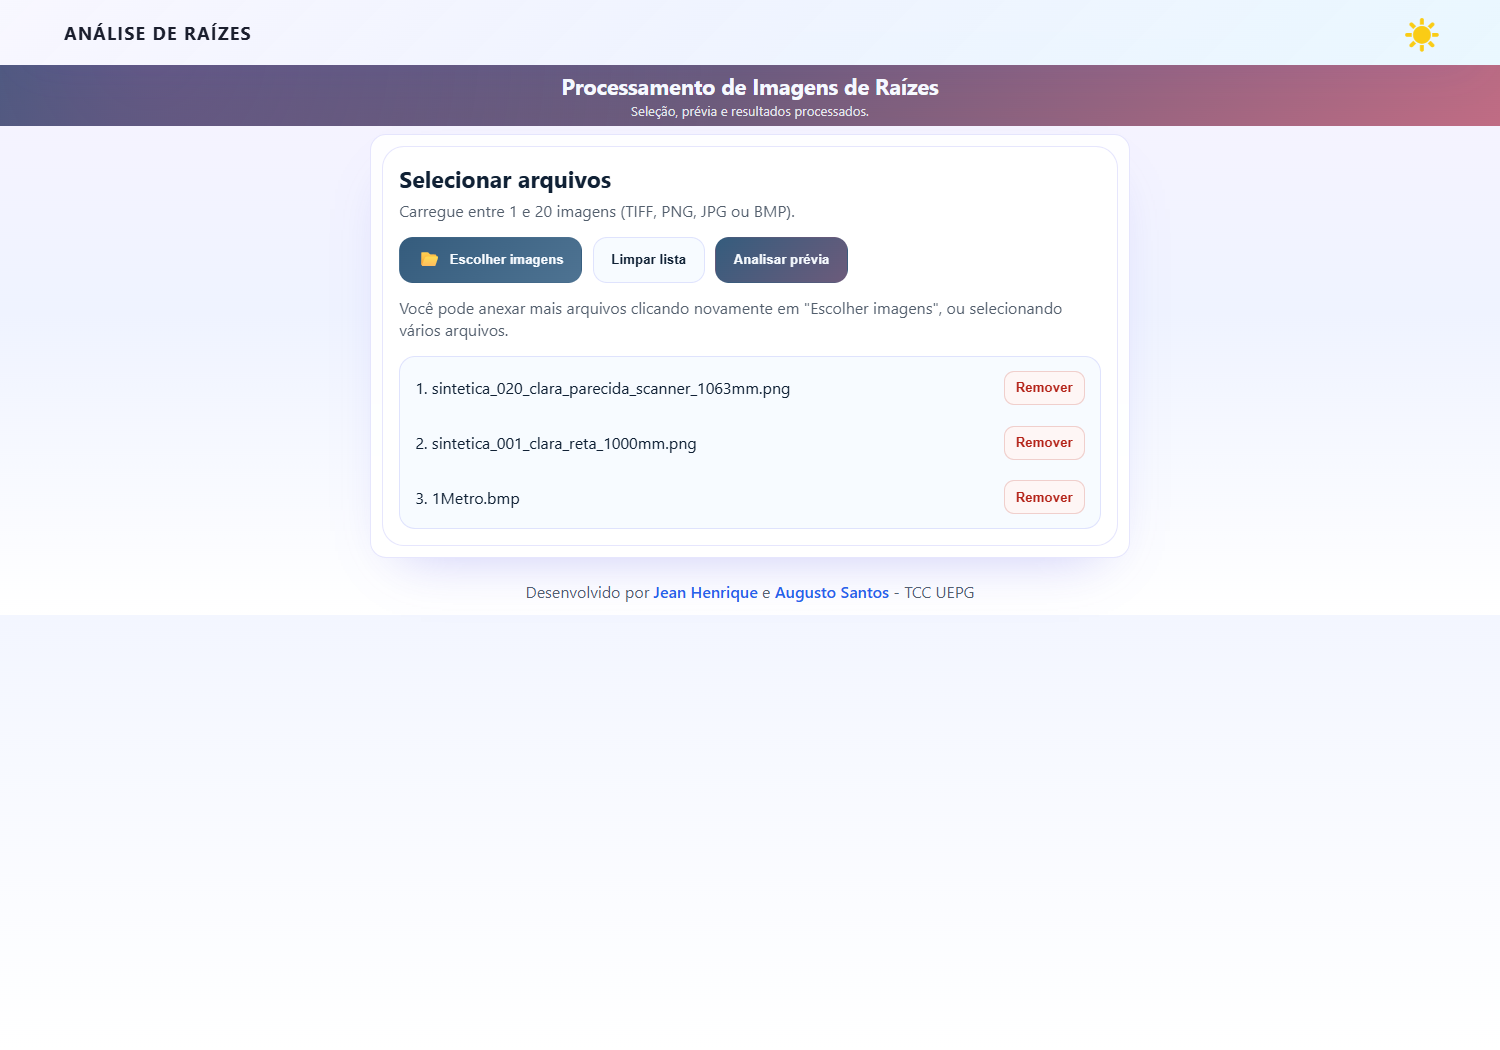
\includegraphics[width=\textwidth,height=0.58\textheight,keepaspectratio]{interface/tela_03_lista_lote.png}
\caption{Lista de imagens selecionadas para processamento em lote.}
\label{fig:ui-lista-lote}
\end{figure}

\subsubsection{DPI, limiar, fundo predominante, histograma e recorte}

Após a seleção de arquivo(s) e clicado em "Analisar prévia", tem-se a Figura \ref{fig:ui-previa} ou a Figura \ref{fig:ui-previa-lote} (para o caso de seleção de mais de uma imagem), onde estão presentes a quantidade de imagem a ser analisada, DPI, o fundo predominante, limiar e histograma. 

\begin{figure}[!htbp]
\centering
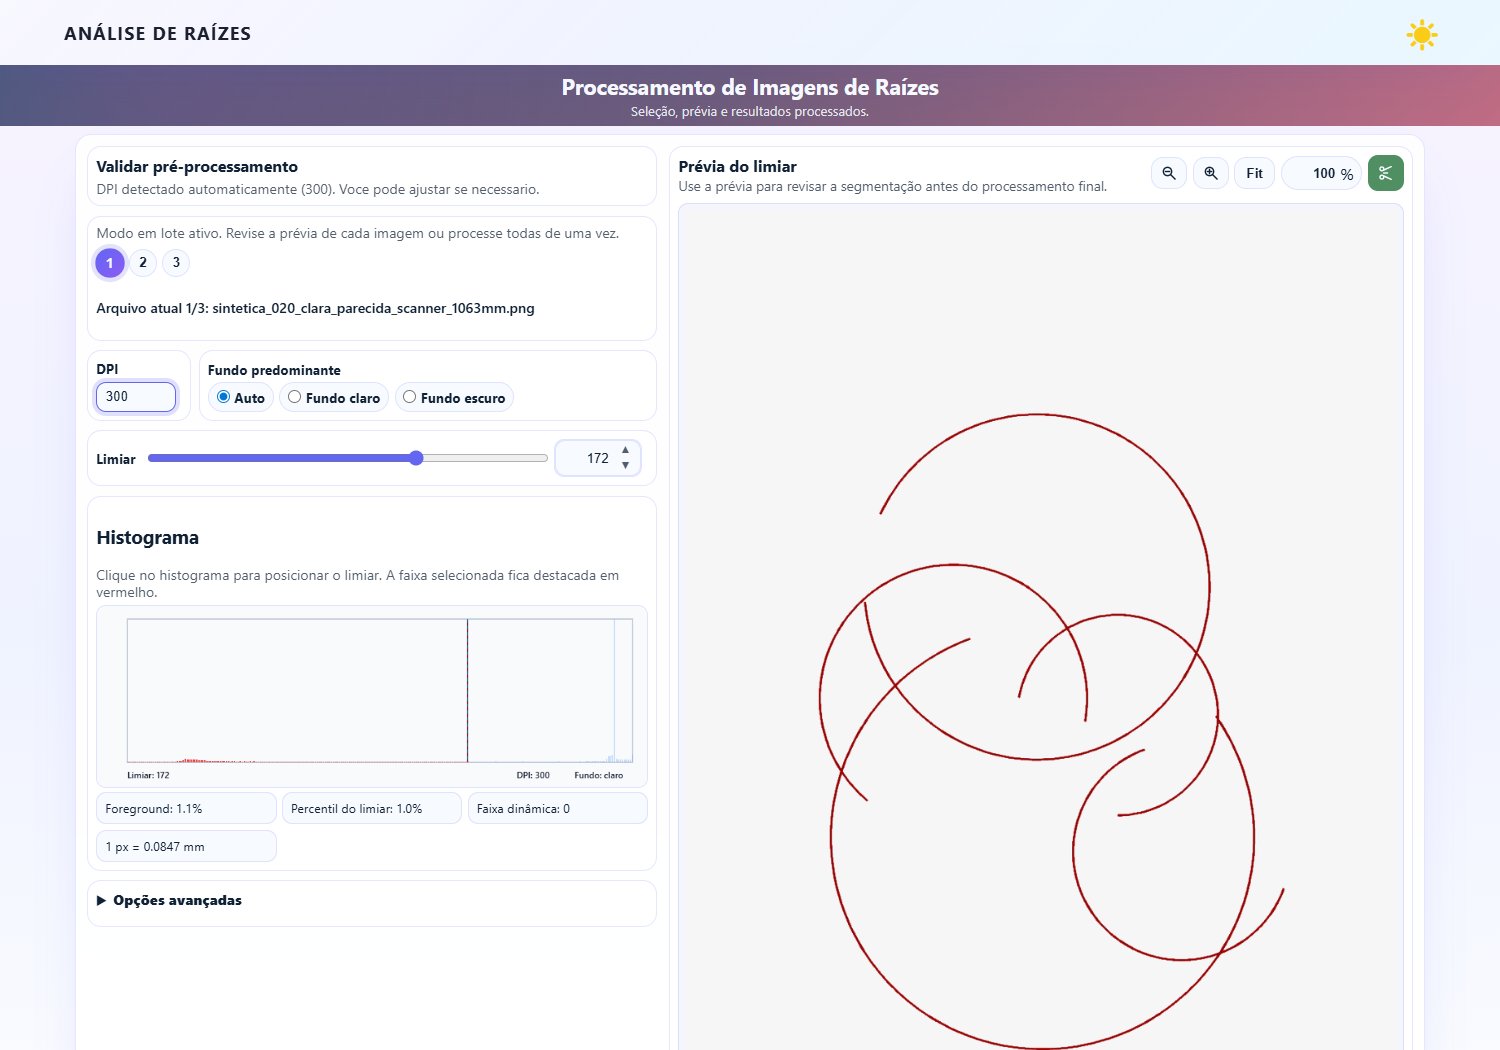
\includegraphics[width=\textwidth,height=0.58\textheight,keepaspectratio]{interface/tela_04_previa_limiar.png}
\caption{Tela de prévia com DPI, limiar, histograma, estatísticas de pré-processamento e sobreposição vermelha da máscara estimada.}
\label{fig:ui-previa}
\end{figure}

\begin{figure}[!htbp]
\centering
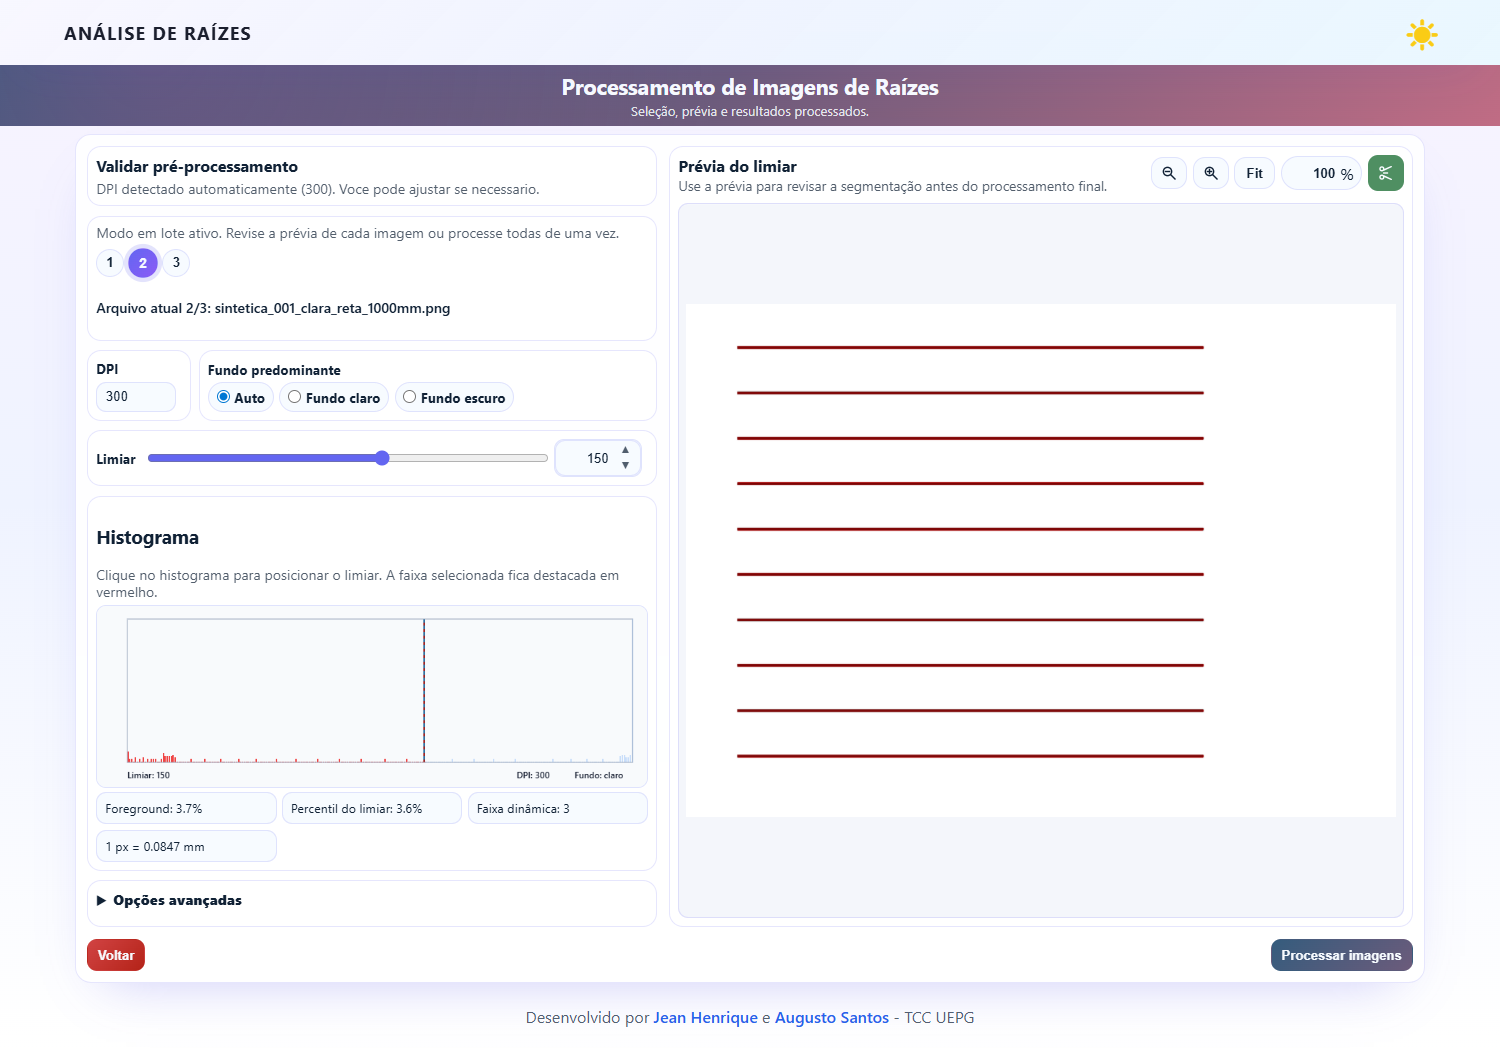
\includegraphics[width=\textwidth,height=0.58\textheight,keepaspectratio]{interface/tela_05_previa_lote.png}
\caption{Navegação entre imagens do lote durante a etapa de prévia.}
\label{fig:ui-previa-lote}
\end{figure}

O DPI é tratado como um parâmetro de medida. Para uma imagem digitalizada a 300 DPI, cada pixel representa aproximadamente:

\[
pixelSize = \frac{25,4}{DPI} = \frac{25,4}{300} = 0,0847\ \text{mm}.
\]

Nessa expressão, $pixelSize$ é o tamanho físico do pixel em milímetros, $DPI$ é a resolução de digitalização em pontos por polegada, e $25,4$ é o número de milímetros contidos em uma polegada. A relação é inversa: quanto maior o DPI, menor a área que cada pixel representa.

É importante ressaltar que, se o DPI estiver errado, o comprimento final também fica errado na mesma proporção. Por isso, o sistema tenta extrair DPI de metadados EXIF, JFIF e TIFF \cite{exif2010,jfif1992}, mas permite entrada manual. Todas as imagens deste trabalho foram processadas com DPI manual de 300 para manter a comparação padronizada.

O limiar é um valor de intensidade do pixel ou tom de cinza escolhido para separar o que será considerado fundo e o que será considerado objeto de interesse para análise, neste trabalho, as raízes. O limiar automático é inicialmente utilizado para separar os pixels em dois grupos a partir do histograma e identificar se a imagem tem fundo predominantemente claro ou escuro. Em uma imagem de fundo claro, a raiz costuma ser mais escura; nesse caso, pixels com intensidade menor ou igual ao limiar entram na máscara (conjunto de pixels considerados raízes). Em uma imagem de fundo escuro, a raiz ou fio costuma ser mais clara; nesse caso, pixels com intensidade maior ou igual ao limiar entram na máscara.

Quando a imagem tem fundo escuro e baixo contraste, o sistema pode aplicar realce morfológico \textit{top-hat} e CLAHE antes da segmentação. O \textit{top-hat} destaca estruturas claras menores que o elemento estruturante, e o CLAHE melhora contraste local sem ampliar demais regiões já claras. Esse modo aparece nos CSVs como \texttt{dark-background-enhanced}.

A função recorte, foi implementada no sistema e está representada pelo ícone verde na Figura \ref{fig:ui-recorte}. Para fazer o recorte, antes do processamento, o usuário seleciona a região de interesse e confirma o procedimento.

\begin{figure}[!htbp]
\centering
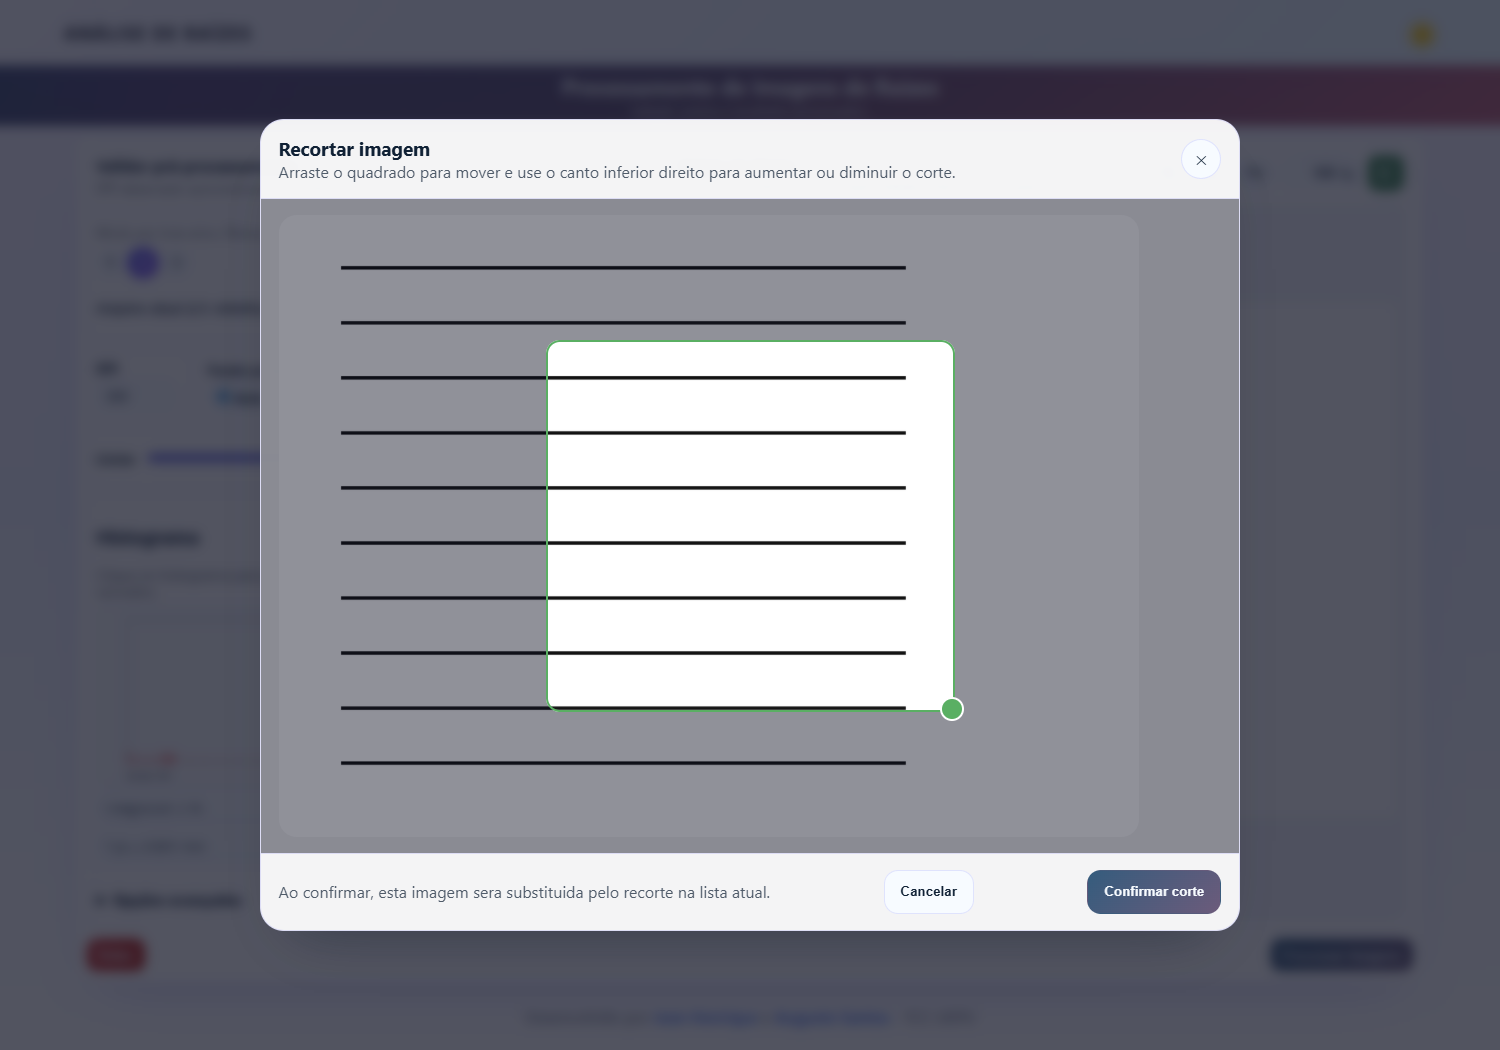
\includegraphics[width=\textwidth,height=0.58\textheight,keepaspectratio]{interface/tela_06_modal_recorte.png}
\caption{Modal de recorte usado para limitar a área analisada antes do processamento.}
\label{fig:ui-recorte}
\end{figure}


\subsubsection{Esqueletização e opções avançadas}

Depois da binarização, a máscara ou o conjunto de pixels representativos das raízes pode conter pontos isolados. Em opções avançadas foram deixadas disponíveis três opções de ajuste neste conjunto: filtro de componentes, podar esqueleto e suavização.

O filtro de componentes conectados identifica grupos de pixels vizinhos usando conectividade 8 \cite{gonzalez2008digital}. A conectividade 8 considera vizinhos horizontais, verticais e diagonais, o que é adequado para raízes finas que podem seguir trajetórias diagonais. Componentes com área menor que um limite são removidos. 

Para a esqueletização o sistema usa \texttt{skimage.morphology.thin}, que aplica afinamento iterativo até obter uma estrutura central. Depois disso, ramos terminais muito curtos podem ser removidos, por meio da opção avançada podar esqueleto.

Outra possibilidade para remoção de pequenos ruídos, que poderiam ser considerados pixels de raízes, é o uso da suavização gaussiana \cite{gonzalez2008digital}.

As três opções avançadas iniciam desmarcadas, de modo que o resultado apresentado por padrão corresponde ao limiar aplicado sobre a imagem, sem etapas adicionais de limpeza. Cabe ao usuário ativar cada ajuste de forma deliberada, o que preserva a rastreabilidade: o CSV exportado registra quais opções estavam ativas em cada medida. Os testes relatados neste trabalho foram executados com as três opções ativadas, conforme descrito na Seção~\ref{sec:validacao}.


\subsubsection{Processamento em lote e feedback}

A Figura \ref{fig:ui-processamento} mostra a tela de bloqueio quando do processamento em lote, evitando que o usuário faça alterações de parâmetros durante este momento. Para ajudar o usuário quanto ao tempo de processamento restante, foi colocada indicação de progresso ao centro.

\begin{figure}[!htbp]
\centering
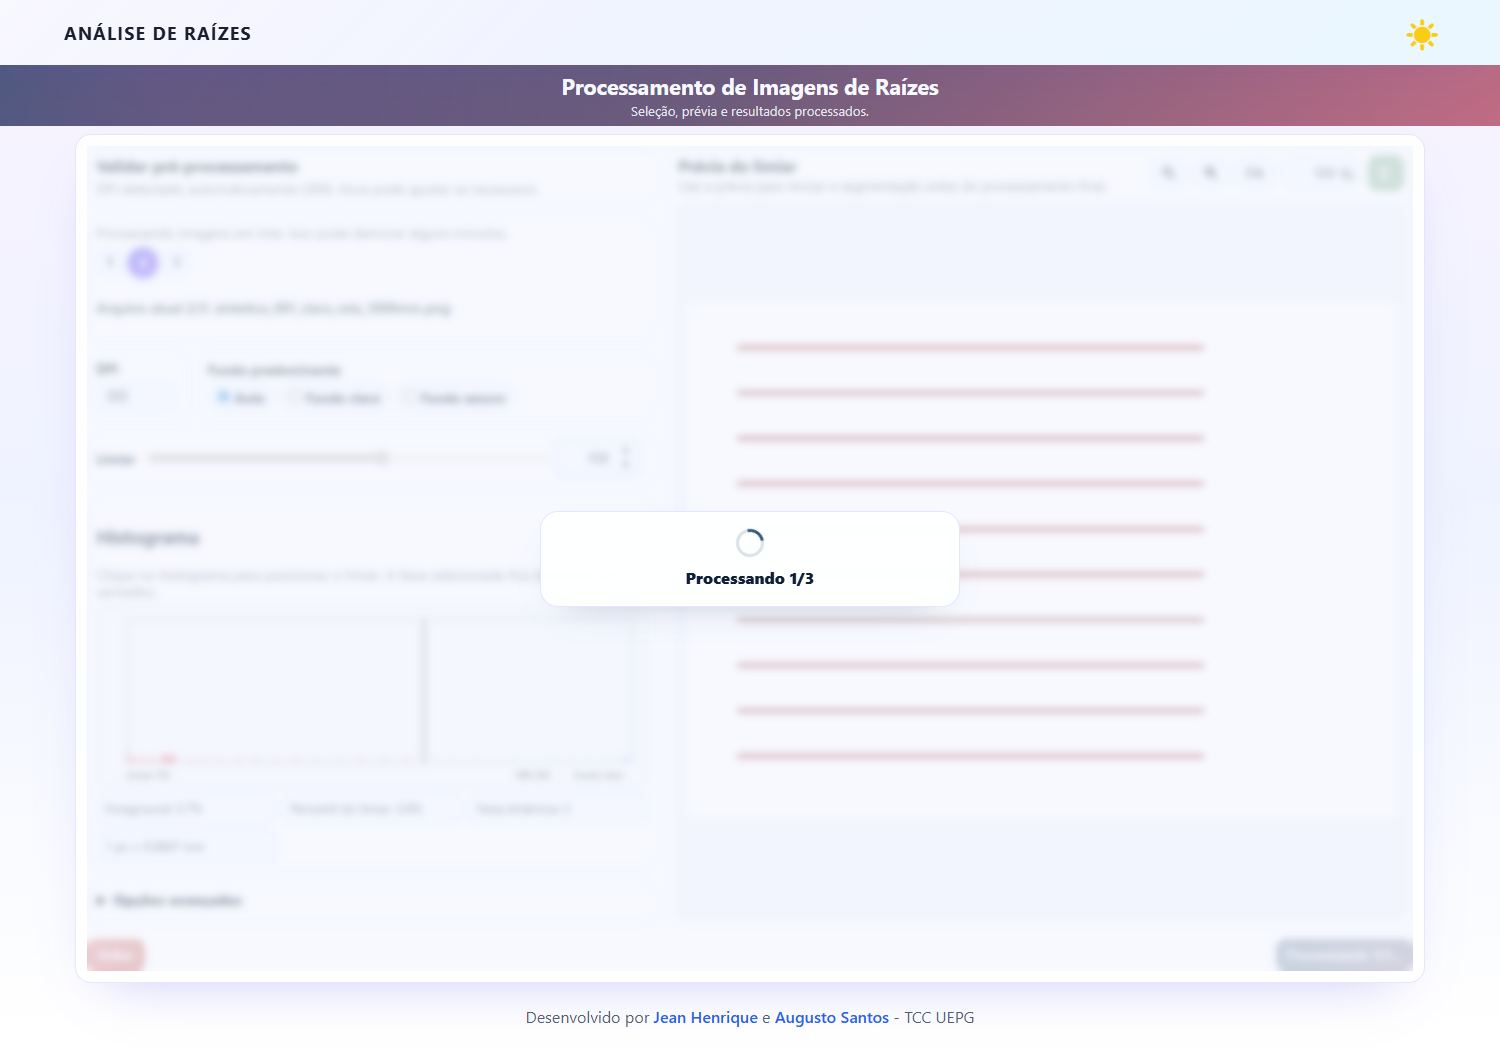
\includegraphics[width=\textwidth,height=0.58\textheight,keepaspectratio]{interface/tela_07_processamento_lote.png}
\caption{Estado de processamento em lote com bloqueio de fluxo e indicação de progresso.}
\label{fig:ui-processamento}
\end{figure}


\subsection{Tela de resultados e rastreabilidade}

Na tela de resultados, Figuras \ref{fig:ui-resultados-lote} e \ref{fig:ui-resultados-scanner}, o sistema apresenta as métricas numéricas e três imagens intermediárias: tons de cinza, segmentada e esqueletizada. Essas saídas são para verificar se a medição é coerente. Uma imagem esqueletizada com muitos ramos em regiões de ruído, tende a ter o comprimento superestimado; por outro lado, se estiver fragmentada ou curta, o comprimento tende a ser subestimado.

As Figuras \ref{fig:ui-mobile} e \ref{fig:ui-ipad} são resultados do comportamento do sistema em diferentes formatos de tela, para celular e tablet, respectivamente.

\begin{figure}[!]
\centering
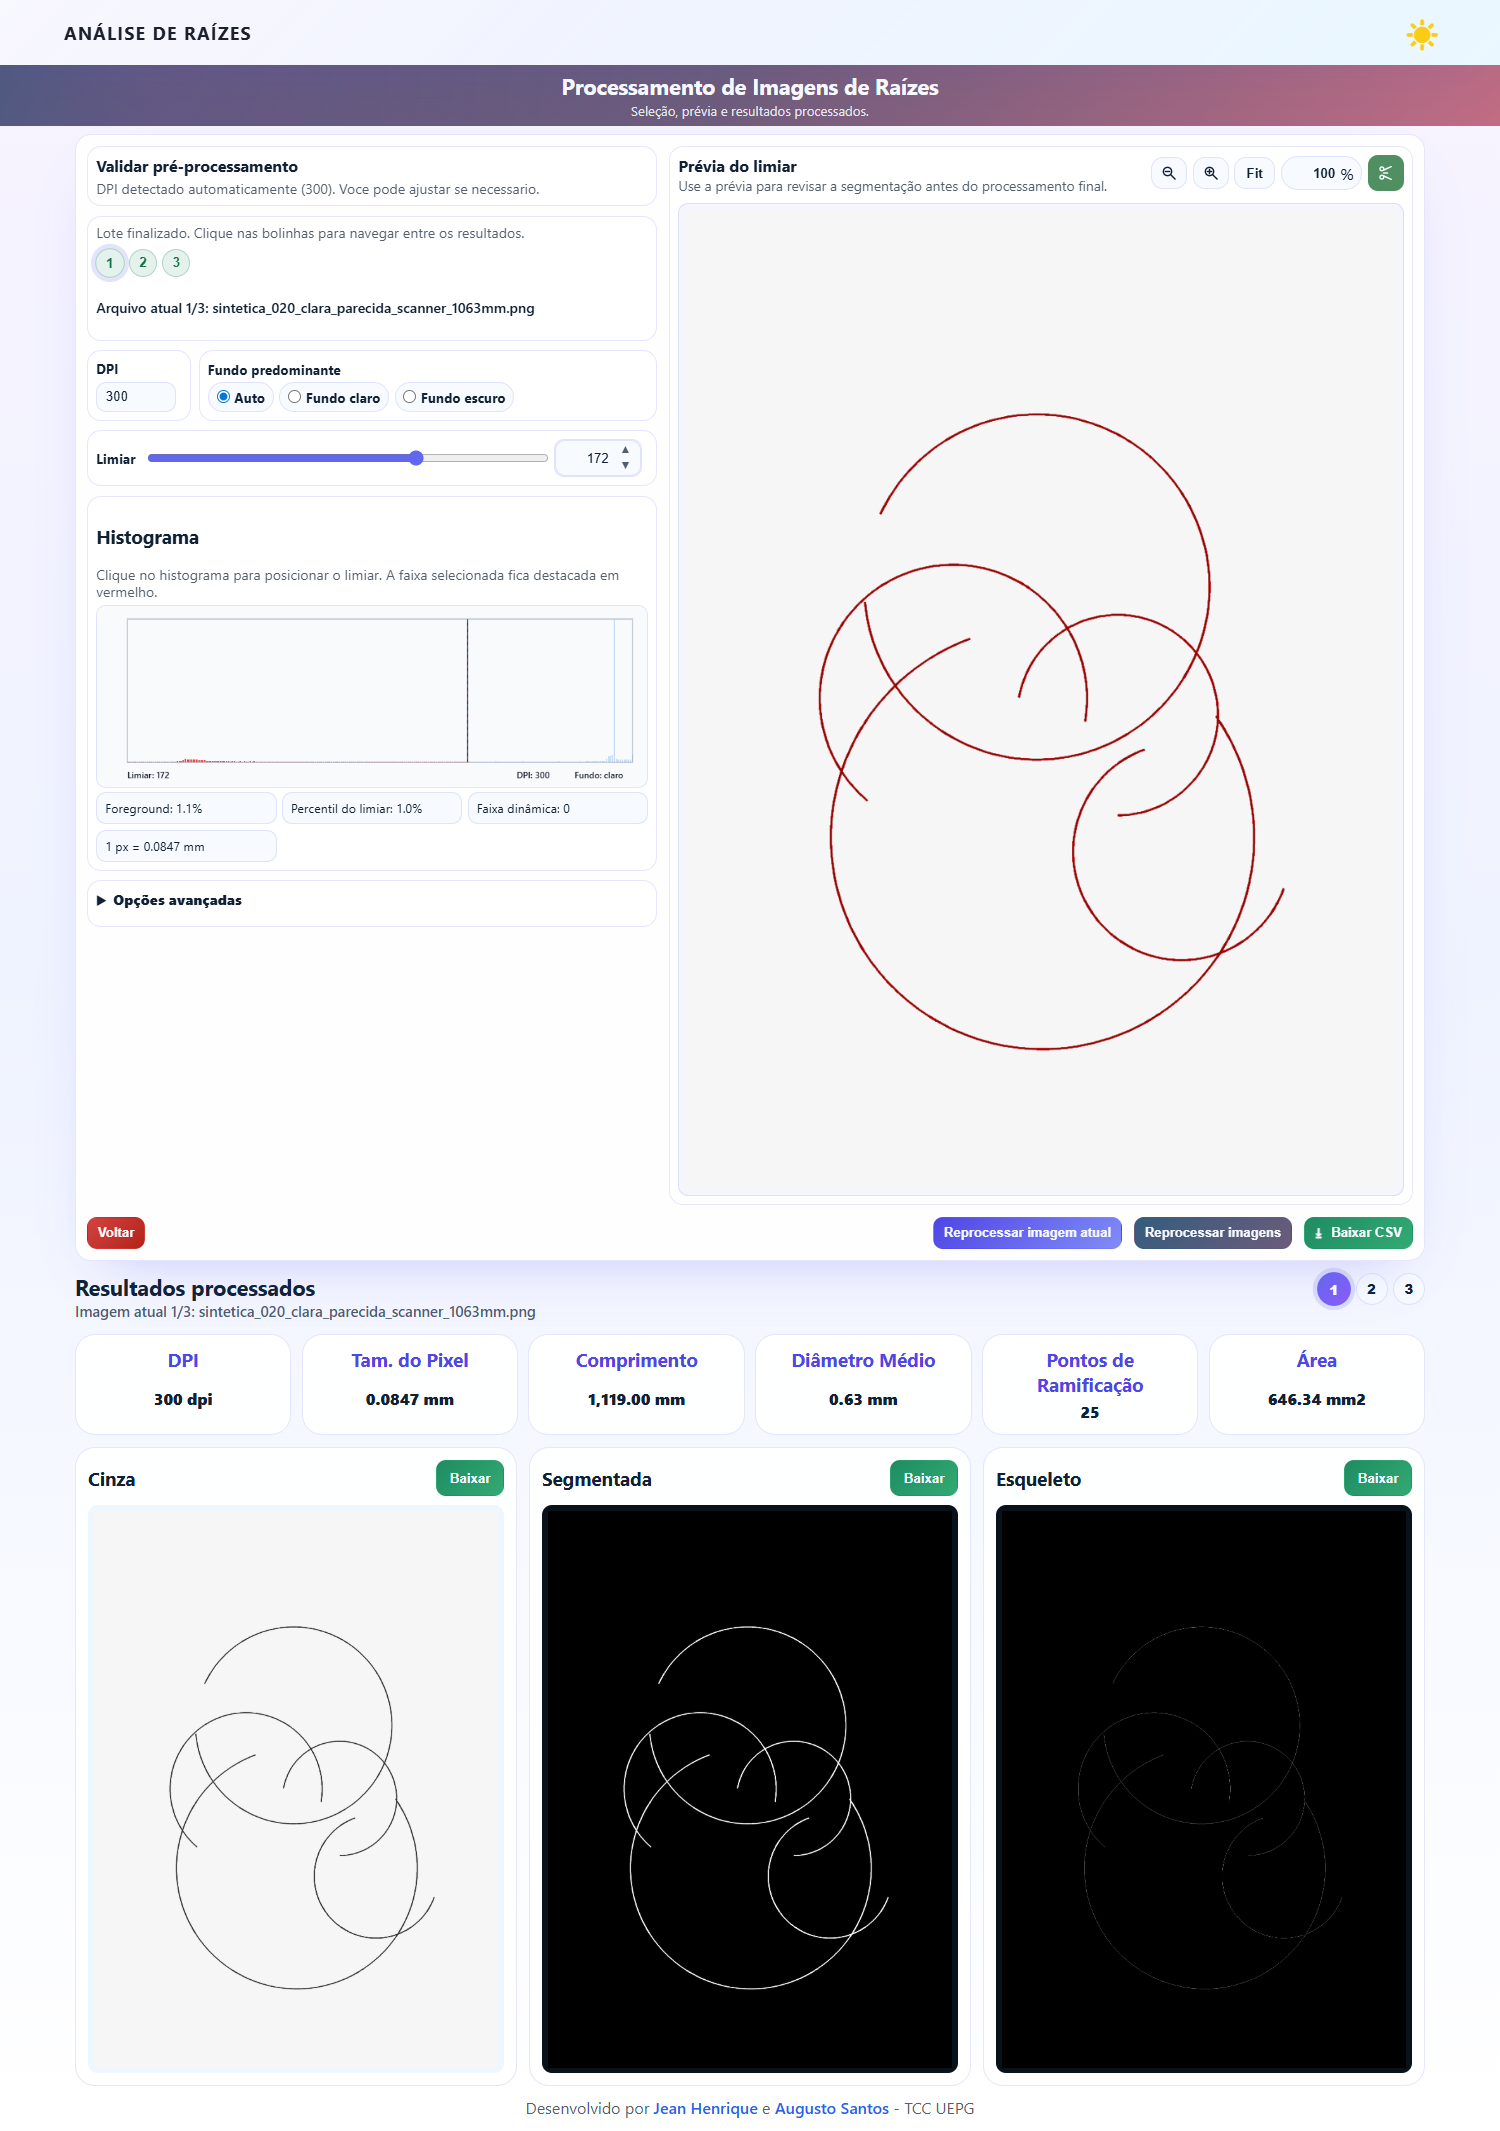
\includegraphics[width=\textwidth,height=0.58\textheight,keepaspectratio]{interface/tela_08_resultados_lote.png}
\caption{Tela de resultados com métricas e imagens intermediárias (tons de cinza, limiarizada e esqueletizada) para uma imagem sintética.}
\label{fig:ui-resultados-lote}
\end{figure}

\begin{figure}[!htbp]
\centering
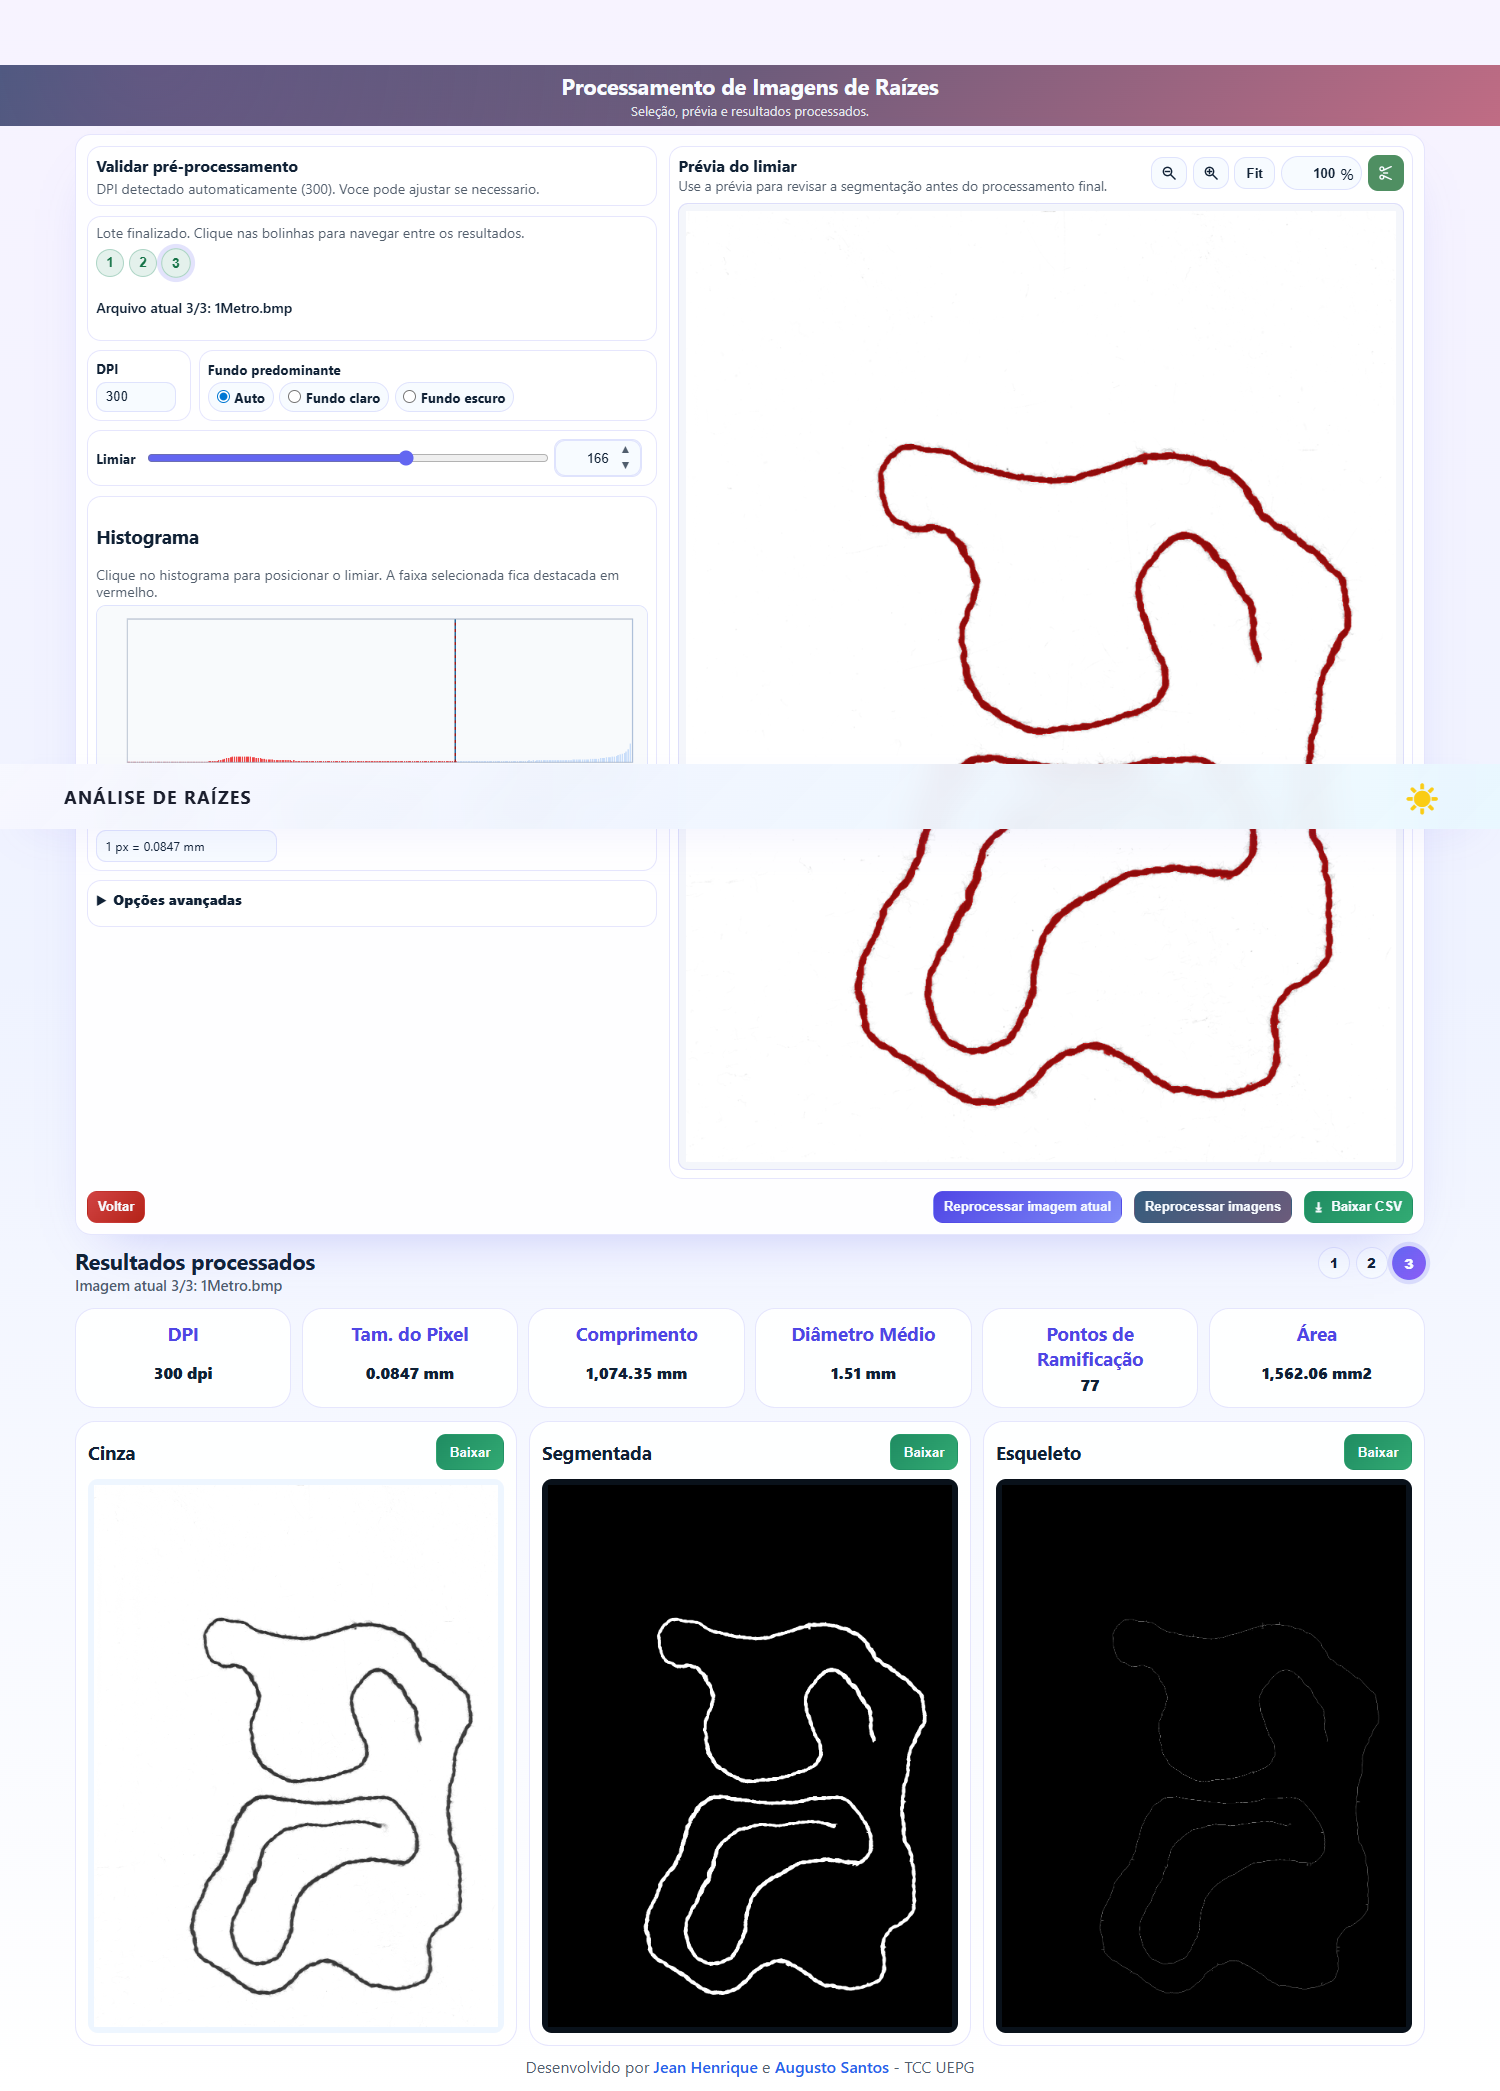
\includegraphics[width=\textwidth,height=0.58\textheight,keepaspectratio]{interface/tela_09_resultados_scanner.png}
\caption{Tela de resultados com métricas e imagens intermediárias (tons de cinza, limiarizada e esqueletizada) para uma imagem de scanner.}
\label{fig:ui-resultados-scanner}
\end{figure}

\subsubsection{Responsividade}

\begin{figure}[!htbp]
\centering
\begin{minipage}[t]{0.31\linewidth}
\centering
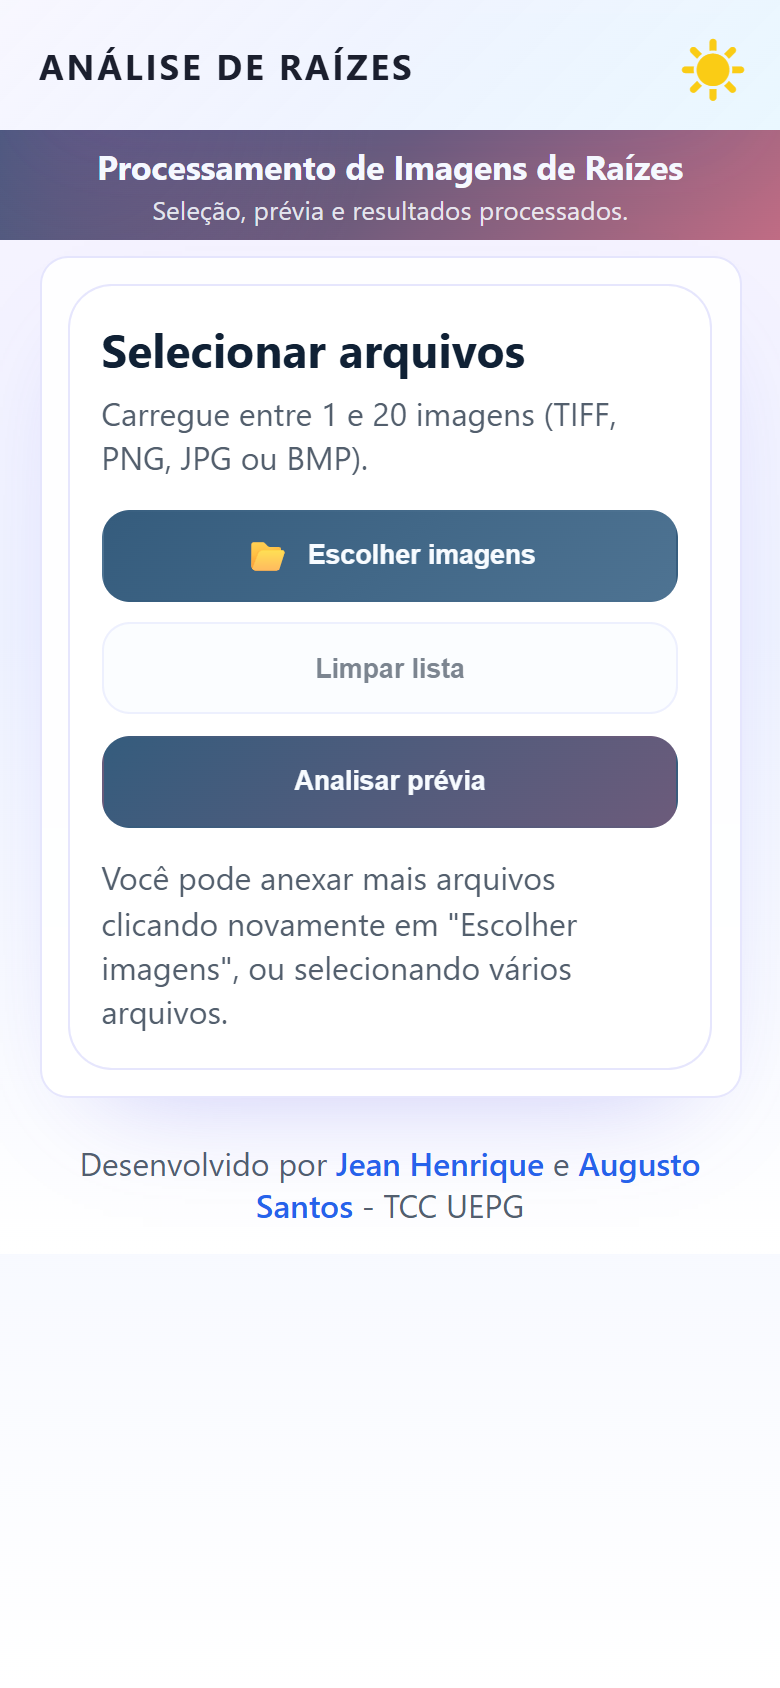
\includegraphics[width=\linewidth,height=0.46\textheight,keepaspectratio]{responsivo/mobile_01_selecao.png}
\end{minipage}
\hfill
\begin{minipage}[t]{0.31\linewidth}
\centering
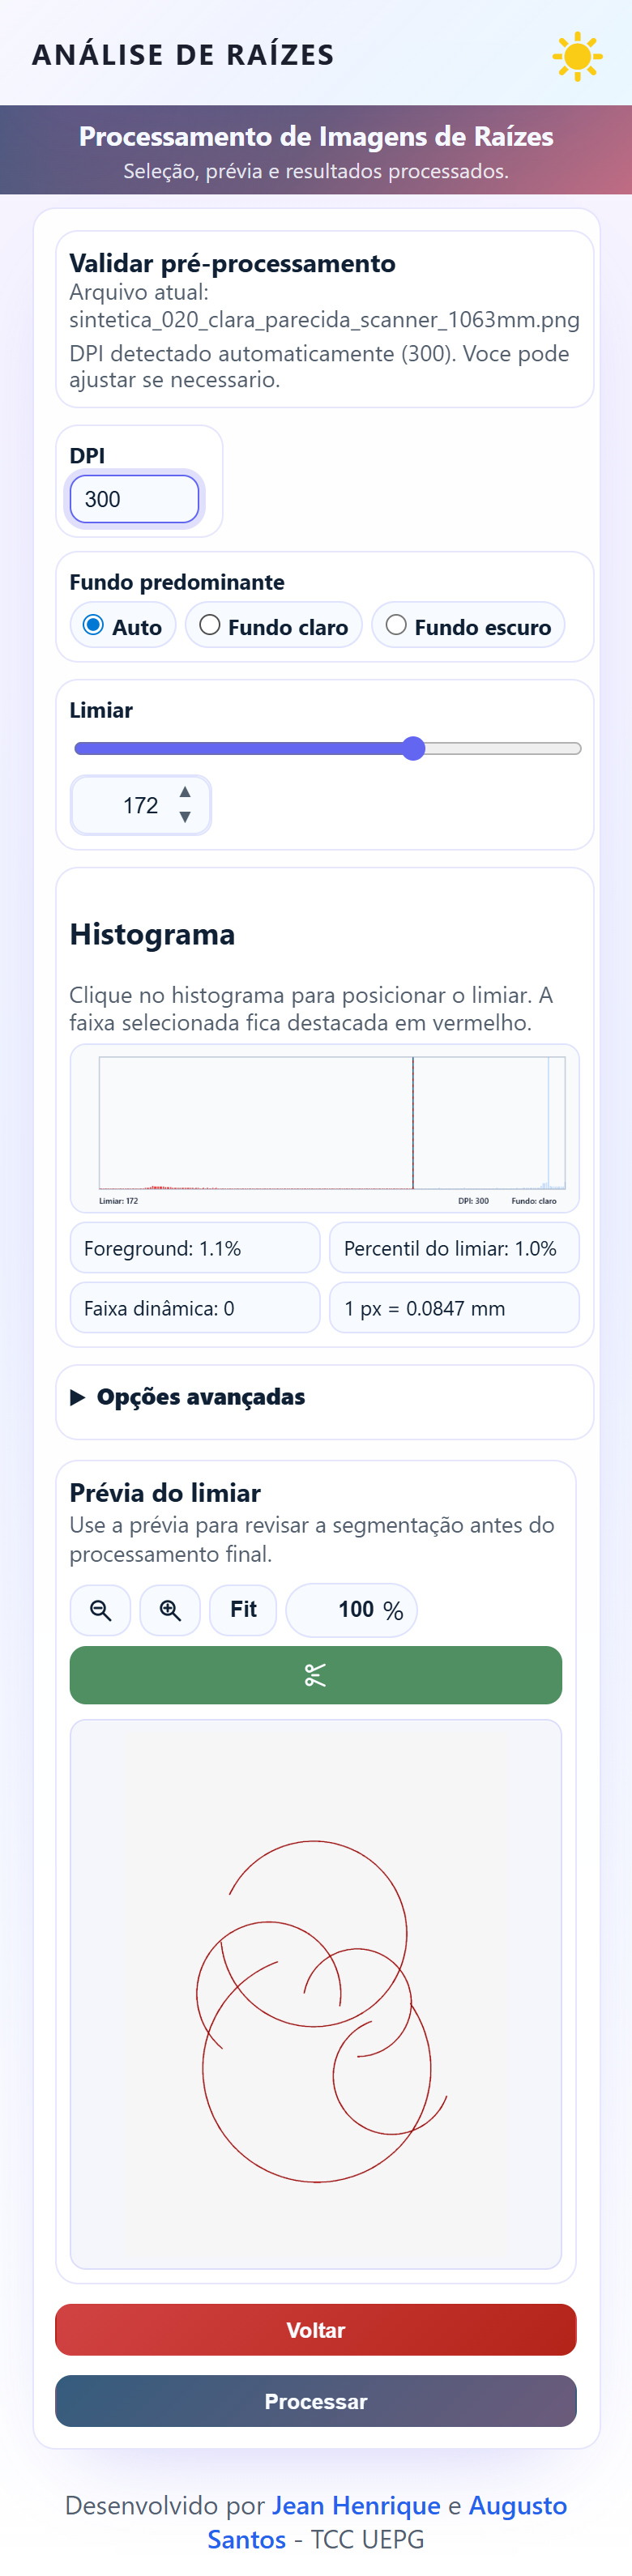
\includegraphics[width=\linewidth,height=0.46\textheight,keepaspectratio]{responsivo/mobile_02_previa.png}
\end{minipage}
\hfill
\begin{minipage}[t]{0.31\linewidth}
\centering
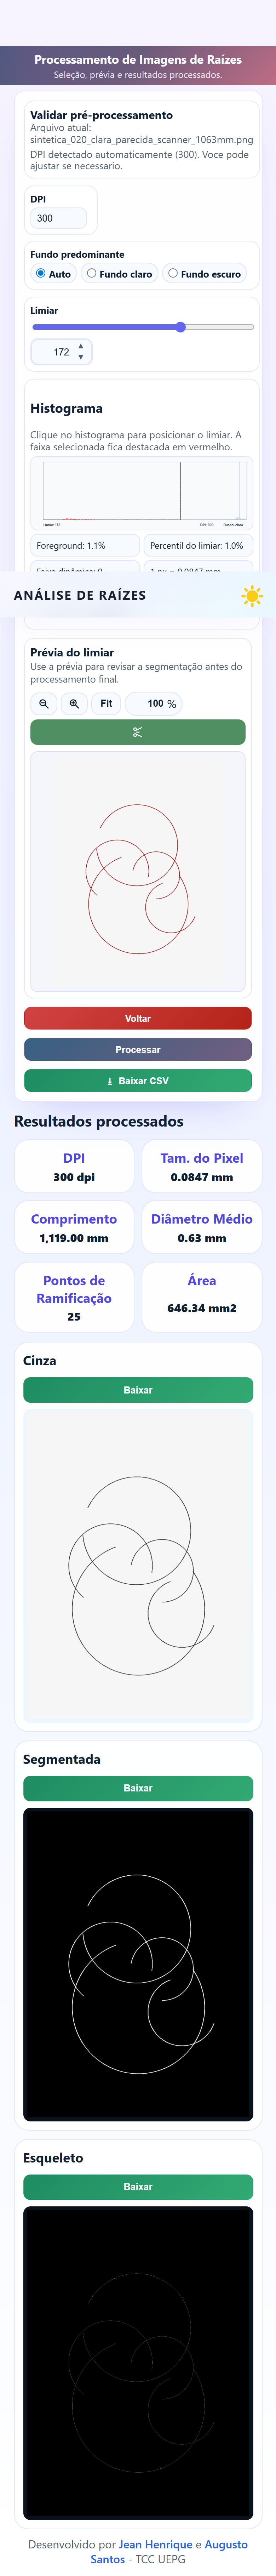
\includegraphics[width=\linewidth,height=0.46\textheight,keepaspectratio]{responsivo/mobile_03_resultados.png}
\end{minipage}
\caption{Interface responsiva em celular: seleção, prévia e resultados.}
\label{fig:ui-mobile}
\end{figure}

\begin{figure}[!htbp]
\centering
\begin{minipage}[t]{0.31\linewidth}
\centering
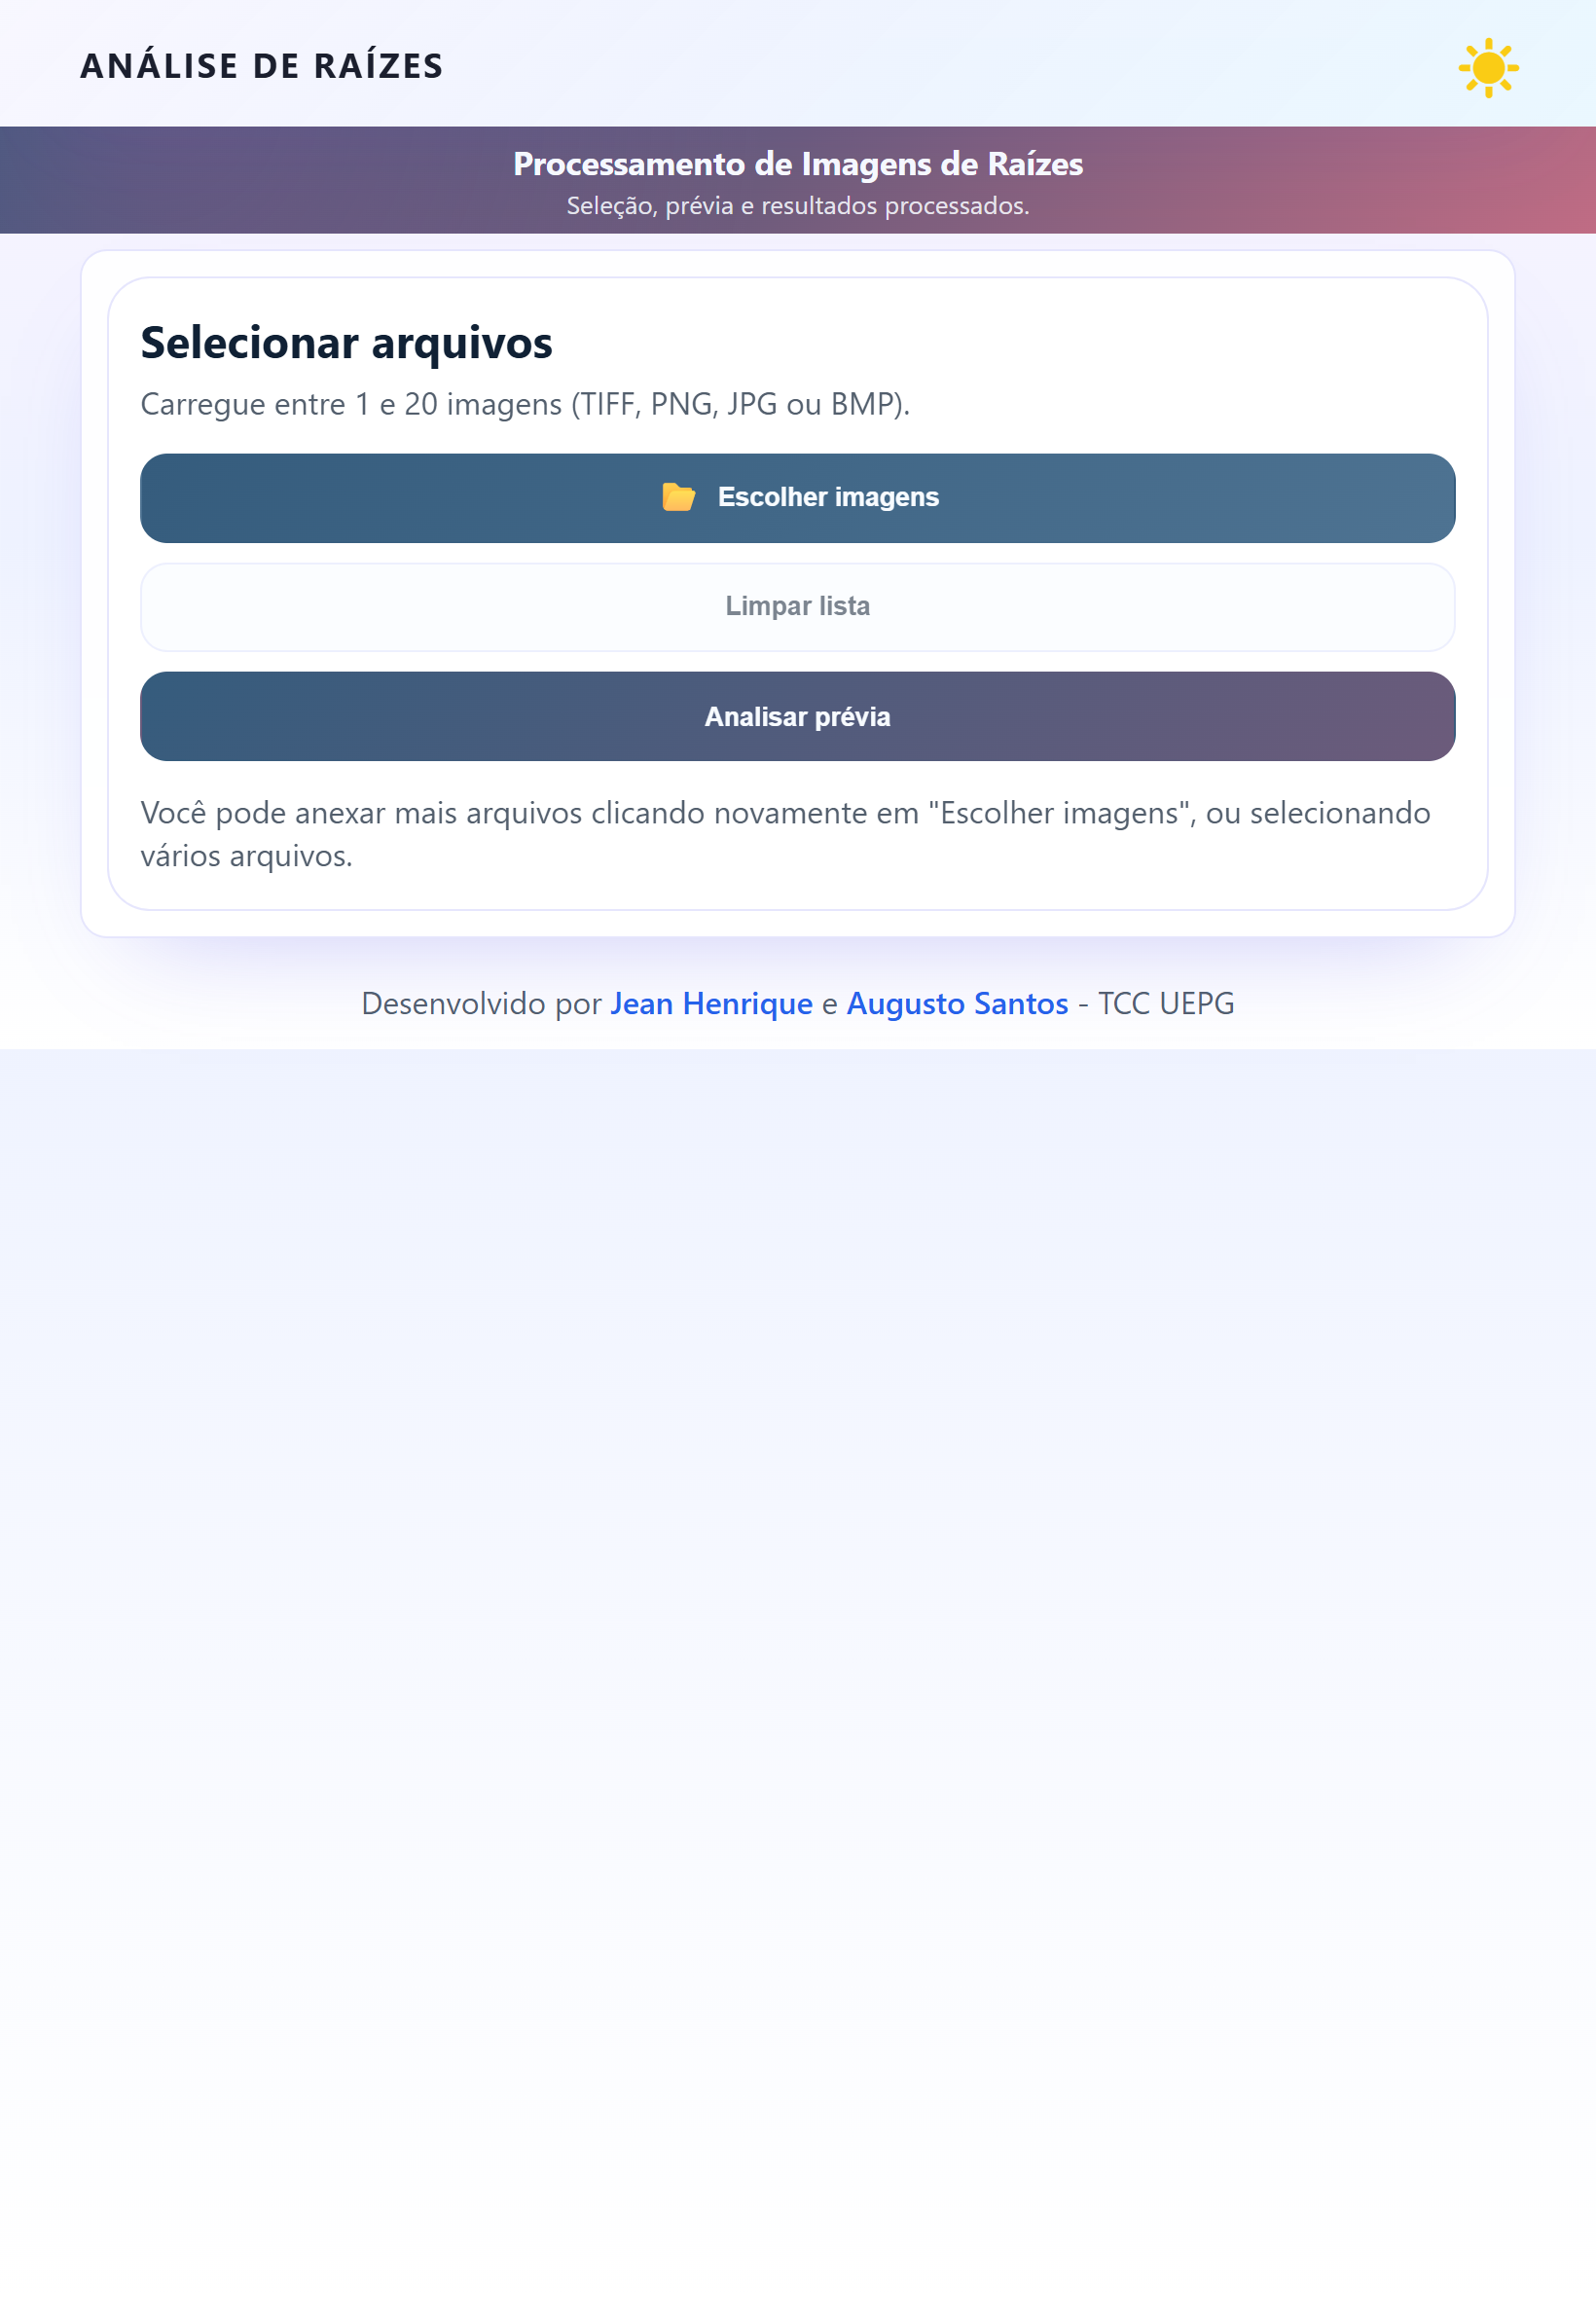
\includegraphics[width=\linewidth,height=0.46\textheight,keepaspectratio]{responsivo/ipad_01_selecao.png}
\end{minipage}
\hfill
\begin{minipage}[t]{0.31\linewidth}
\centering
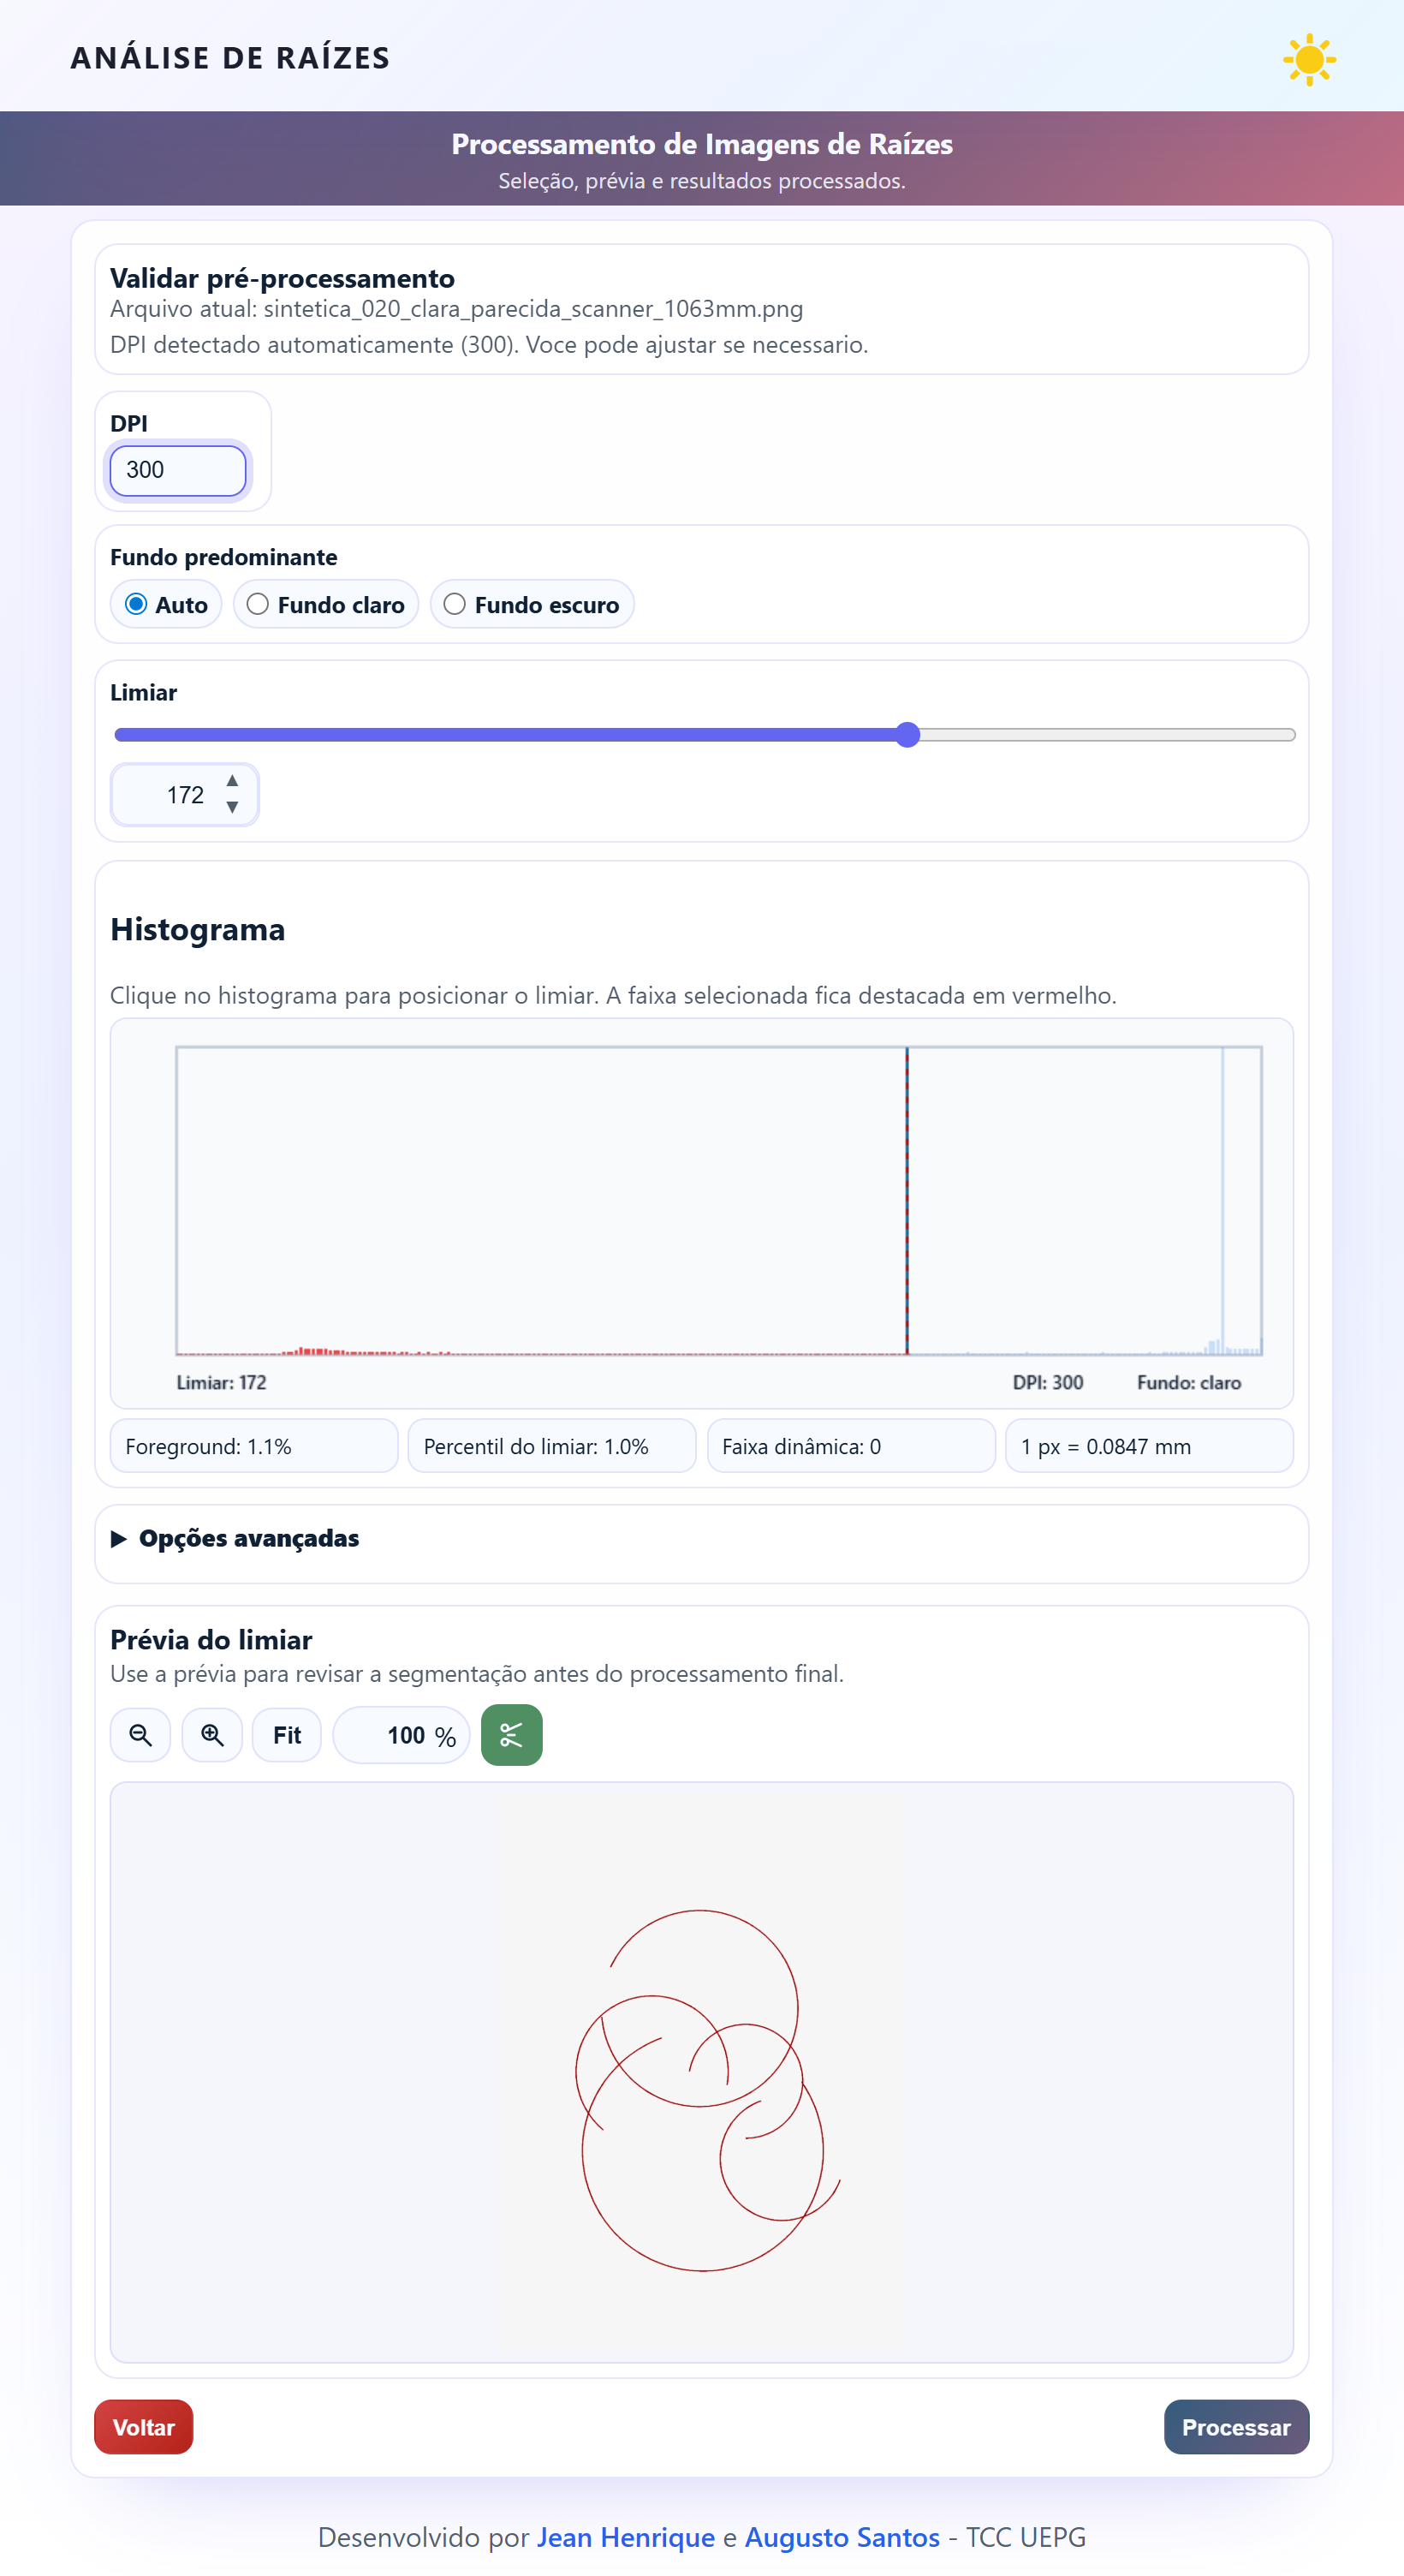
\includegraphics[width=\linewidth,height=0.46\textheight,keepaspectratio]{responsivo/ipad_02_previa.png}
\end{minipage}
\hfill
\begin{minipage}[t]{0.31\linewidth}
\centering
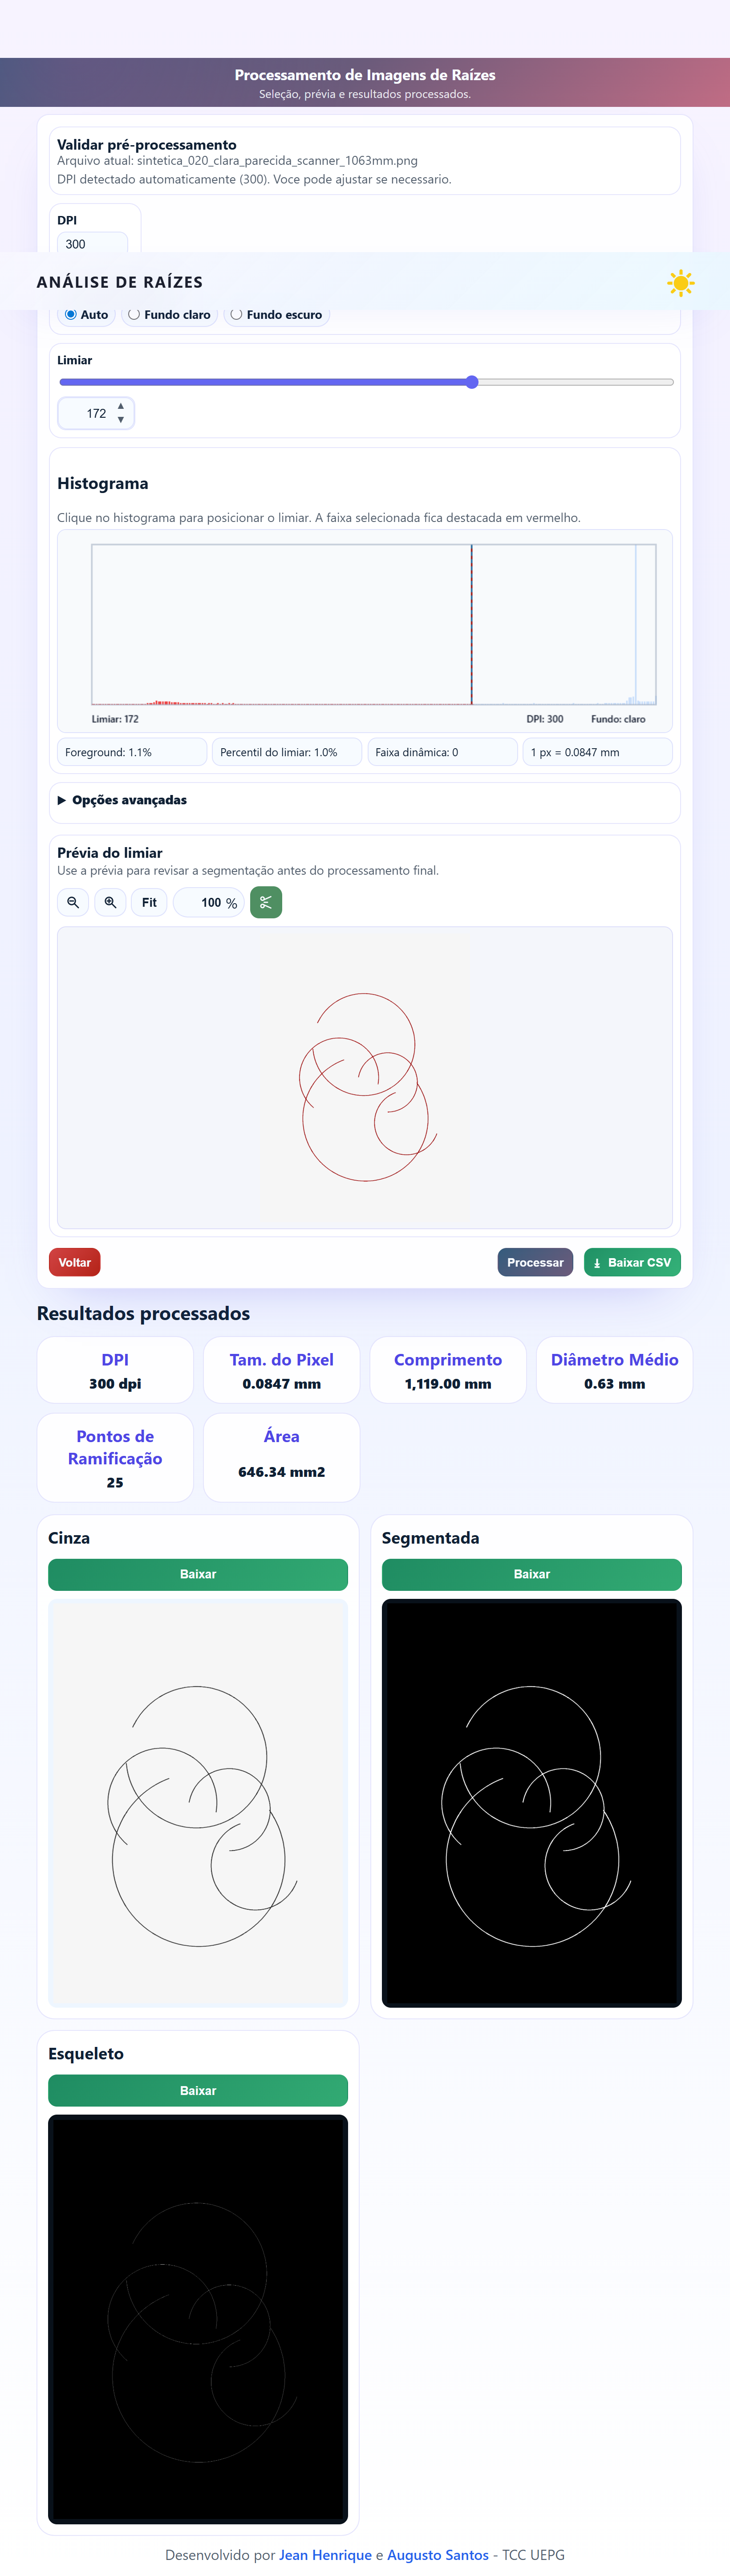
\includegraphics[width=\linewidth,height=0.46\textheight,keepaspectratio]{responsivo/ipad_03_resultados.png}
\end{minipage}
\caption{Interface responsiva em iPad/tablet: seleção, prévia e resultados.}
\label{fig:ui-ipad}
\end{figure}

Enquanto em desktop, por exemplo, Figura \ref{fig:ui-resultados-scanner}, os controles e a prévia podem aparecer lado a lado, favorecendo comparação visual. Em celulares (Figura \ref{fig:ui-mobile}) e tablets (Figura \ref{fig:ui-ipad}), os mesmos elementos estão empilhados em uma coluna, preservando a ordem do fluxo, sem sobreposição de controles e mantendo os campos de DPI e limiar acessíveis.

\subsection{Análise Estatística}

As Figuras \ref{fig:proc-sintetica}, \ref{fig:proc-jean} e \ref{fig:proc-teruo}, apresentadas na Seção~\ref{sec:etapas}, trazem exemplos de saída para cada conjunto analisado e permitem acompanhar visualmente o que ocorre entre a imagem de entrada e o valor medido. Na Figura \ref{fig:proc-sintetica}, o contraste é alto e a máscara reproduz a estrutura desenhada quase sem perda, o que é coerente com o erro de poucos por cento observado no grupo sintético. Na Figura \ref{fig:proc-jean}, a estrutura é fina e o esqueleto preserva a trajetória, mas pequenas inclusões próximas às extremidades já são visíveis na máscara, o que explica a tendência de superestimação nesse conjunto. Na Figura \ref{fig:proc-teruo}, a amostra de 7487 mm apresenta segmentação limpa e esqueleto contínuo, e é justamente esse comportamento que corresponde aos casos do grupo Teruo com erro abaixo de 5\%. Essas mesmas imagens são retomadas na discussão dos desvios, na Seção \ref{sec:sintese}, pois são o principal instrumento de verificação disponível ao usuário quando um valor medido parece incoerente.


As Tabelas \ref{tab:sinteticas}, \ref{tab:jean}, \ref{tab:teruo} e \ref{tab:stats} foram todas obtidas com a mesma configuração descrita na Seção~\ref{sec:validacao}: limiar automático, suavização, filtragem de componentes e poda de esqueleto ativadas, e DPI fixado manualmente em 300. A coluna \emph{Limiar} das tabelas por imagem traz o valor que o algoritmo automático calculou para aquela imagem, e não um valor escolhido pelo operador.

\subsubsection{Análises das imagens sintéticas}

As imagens sintéticas testam o comportamento do algoritmo em condições controladas. A Tabela~\ref{tab:sinteticas} mostra que quase todos os casos ficaram abaixo de 10\% de erro. O pior caso foi a imagem de cruzamentos, com -10,31\%, seguida da imagem de fragmentos curtos e esparsos, com -9,57\%. Esses casos são coerentes com limitações esperadas: cruzamentos e fragmentos dificultam a representação do comprimento real por uma linha central única \cite{bucksch2014image}.

\begin{table}[!htbp]
\centering
\caption{Resultados das imagens sintéticas.}
\label{tab:sinteticas}
\resizebox{\textwidth}{!}{
\begin{tabular}{lrrrr}
\toprule
Amostra & Referência (mm) & Medido (mm) & Erro (\%) & Limiar \\
\midrule
S01 reta & 1000 & 994,83 & -0,52 & 145 \\
S02 curva contínua & 1500 & 1495,89 & -0,27 & 143 \\
S03 fragmentada & 7000 & 7122,87 & 1,76 & 113 \\
S04 fragmentada com ruído & 3000 & 2979,88 & -0,67 & 111 \\
S05 rede densa & 6600 & 6481,16 & -1,80 & 114 \\
S06 raízes espessas & 2500 & 2443,99 & -2,24 & 121 \\
S07 vertical & 2200 & 2166,07 & -1,54 & 114 \\
S08 diagonal & 1800 & 1738,70 & -3,41 & 113 \\
S09 clara fragmentada & 4200 & 4245,73 & 1,09 & 147 \\
S10 baixo contraste & 2000 & 2091,03 & 4,55 & 42 \\
S11 clara com ruído & 3500 & 3609,58 & 3,13 & 150 \\
S12 cruzamentos & 5200 & 4663,86 & -10,31 & 114 \\
S13 fina & 1200 & 1266,58 & 5,55 & 95 \\
S14 arcos longos & 7000 & 7105,28 & 1,50 & 113 \\
S15 curtas esparsas & 2800 & 2532,18 & -9,57 & 109 \\
S16 circular contínua & 1000 & 1055,52 & 5,55 & 144 \\
S17 laços aninhados & 1442 & 1517,59 & 5,24 & 145 \\
S18 espiral contínua & 2609 & 2751,64 & 5,47 & 145 \\
S19 fragmentos circulares & 3600 & 3567,24 & -0,91 & 113 \\
S20 parecida com scanner & 1063 & 1119,06 & 5,27 & 152 \\
\bottomrule
\end{tabular}}
\end{table}

\subsubsection{Análises das imagens de scanner Jean}

As imagens de scanner Jean, compostas por fios de náilon, apresentaram erro absoluto médio de 14,65\%, Tabela \ref{tab:jean}. Por se tratar de estrutura de espessura uniforme e sem ramificação, esse conjunto isola o comportamento geométrico do algoritmo: os desvios observados não podem ser atribuídos a cruzamentos ou a variação de espessura da amostra. O principal desvio foi a imagem contínua de 0,36 m, medida como 593,06 mm, com erro de 64,74\%. Como a referência é curta, pequenas inclusões extras de estrutura ou ruído geram erro percentual alto. Excluindo esse caso, os demais erros ficaram entre 2,33\% e 12,31\%.

\begin{table}[!htbp]
\centering
\caption{Resultados das imagens Jean.}
\label{tab:jean}
\resizebox{\textwidth}{!}{
\begin{tabular}{llrrrr}
\toprule
Subgrupo & Arquivo & Referência (mm) & Medido (mm) & Erro (\%) & Limiar \\
\midrule
Contínuo & 0,215Metro.bmp & 215 & 241,47 & 12,31 & 164 \\
Contínuo & 0,36Metro.bmp & 360 & 593,06 & 64,74 & 164 \\
Contínuo & 0,5Metro.bmp & 500 & 544,37 & 8,87 & 165 \\
Contínuo & 1Metro.bmp & 1000 & 1071,42 & 7,14 & 163 \\
Picotado & 0,27Metro.bmp & 270 & 278,43 & 3,12 & 171 \\
Picotado & 0,37Metro.bmp & 370 & 406,56 & 9,88 & 172 \\
Picotado & 1,6Metro.bmp & 1600 & 1637,27 & 2,33 & 170 \\
Picotado & 1Metro.bmp & 1000 & 1088,07 & 8,81 & 164 \\
\bottomrule
\end{tabular}}
\end{table}

Esse resultado sugere que o pipeline tem bom comportamento para a maior parte das imagens Jean, mas é sensível a imagens curtas quando a segmentação captura pixels adicionais. A interface de prévia é importante nesses casos, pois permite identificar visualmente se a máscara extrapolou a estrutura esperada.

\subsubsection{Análises das imagens de scanner Teruo}

As imagens de scanner Teruo tiveram MAE de 13,03\%, Tabela \ref{tab:teruo}. Quatro das oito imagens ficaram dentro de 5\%, e seis ficaram dentro de 10\%. Os maiores desvios foram para as imagens  \texttt{37 - 3000.bmp}, com superestimação de 50,66\%, e \texttt{32 - 3000.bmp}, com subestimação de -29,13\%. Esses dois casos concentraram os principais desvios do grupo.

\begin{table}[!htbp]
\centering
\caption{Resultados das imagens Teruo.}
\label{tab:teruo}
\resizebox{\textwidth}{!}{
\begin{tabular}{lrrrr}
\toprule
Arquivo & Referência (mm) & Medido (mm) & Erro (\%) & Limiar \\
\midrule
1225.bmp & 1225 & 1230,50 & 0,45 & 17,00 \\
1634.bmp & 1634 & 1506,95 & -7,78 & 19,04 \\
2000.bmp & 2000 & 1964,03 & -1,80 & 9,00 \\
32 - 3000.bmp & 3000 & 2125,99 & -29,13 & 14,28 \\
37 - 3000.bmp & 3000 & 4519,80 & 50,66 & 9,00 \\
6639.bmp & 6639 & 6106,45 & -8,02 & 33,00 \\
7000.bmp & 7000 & 6845,08 & -2,21 & 11,00 \\
7487.bmp & 7487 & 7174,06 & -4,18 & 33,00 \\
\bottomrule
\end{tabular}}
\end{table}

\subsubsection{Peso das correções heurísticas nos resultados}
\label{sec:correcoes}

As correções descritas na Seção~\ref{sec:validacao} não foram acionadas de maneira uniforme. Nas 20 imagens sintéticas e nas 8 imagens de scanner Jean, nenhuma correção foi aplicada: os valores dessas tabelas são o comprimento geométrico do esqueleto. Já no conjunto de scanner Teruo, 6 das 8 imagens receberam alguma intervenção, sendo 4 pela regra \texttt{dense-graph} e 2 pela regra de fragmentação. O realce de fundo escuro atuou em 6 das 8 imagens desse mesmo grupo.

A Tabela~\ref{tab:correcoes} compara, para essas imagens, o comprimento antes e depois da correção. A diferença é grande: sem as correções, o erro absoluto médio do grupo Teruo seria de 55,06\%, contra os 13,03\% relatados. Em \texttt{2000.bmp}, o esqueleto bruto mediu 5643,71 mm para uma referência de 2000 mm, um erro de 182,19\%, reduzido a $-1,80$\% após a correção; em \texttt{7000.bmp}, o caminho foi inverso, de $-64,47$\% para $-2,21$\%.

\vspace{5mm}

\begin{table}[!htbp]
\centering
\caption{Imagens do grupo Teruo em que houve correção de comprimento.}
\label{tab:correcoes}
\resizebox{\textwidth}{!}{
\begin{tabular}{lrrrrl}
\toprule
Arquivo & Referência (mm) & Bruto (mm) & Corrigido (mm) & Erro bruto (\%) & Correção aplicada \\
\midrule
2000.bmp & 2000 & 5643,71 & 1964,03 & 182,19 & \texttt{dense-graph} \\
7000.bmp & 7000 & 2486,96 & 6845,08 & -64,47 & \texttt{fragmented-components} \\
6639.bmp & 6639 & 9812,51 & 6106,45 & 47,80 & \texttt{dense-graph} \\
37 - 3000.bmp & 3000 & 4898,68 & 4519,80 & 63,29 & \texttt{dense-graph} \\
32 - 3000.bmp & 3000 & 1387,86 & 2125,99 & -53,74 & \texttt{fragmented-components} \\
7487.bmp & 7487 & 9040,96 & 7174,06 & 20,76 & \texttt{dense-graph} \\
\bottomrule
\end{tabular}}
\end{table}

Esse comportamento precisa ser lido com cautela. As correções foram calibradas de forma empírica e melhoram o resultado nas imagens em que a segmentação falhou de modo característico, mas não derivam de um modelo geométrico da estrutura da raiz. Elas indicam, sobretudo, que a segmentação dessas imagens não representou bem a estrutura real: o esqueleto bruto ora formou malha, ora fragmentou. O caminho mais sólido para esse tipo de imagem é melhorar a aquisição e a segmentação, e não ampliar o número de correções sobre o valor medido.

As correções atuam de forma automática e sem intervenção do usuário, e recuperaram medidas em dois modos conhecidos de falha da segmentação: esqueleto adensado por supersegmentação e máscara fragmentada. O ganho observado nas imagens de scanner é expressivo, mas seus limites de acionamento foram ajustados sobre o próprio conjunto de validação, e a amostra \texttt{1634.bmp} ficou a menos de 4\% do limite de disparo, o que indica sensibilidade a pequenas variações de aquisição. Há ainda uma limitação conceitual: a regra de densidade não distingue um esqueleto adensado por supersegmentação de um sistema radicular legitimamente ramificado, de modo que amostras muito ramificadas podem ser subestimadas sem sinalização. Conclui-se, portanto, que o sistema é capaz de recuperar medidas em imagens de qualidade inferior às condições ideais, mas que essa capacidade ainda não pode ser generalizada para amostras de outra origem sem validação independente.

A Tabela~\ref{tab:stats} resume os resultados estatísticos obtidos. O conjunto sintético obteve MAE de 3,52\%, ou seja, em 19 das 20 imagens os resultados estiveram dentro de 10\%. Isso indica que o cálculo geométrico do esqueleto é consistente quando a entrada é controlada. Nas imagens reais, o erro aumentou: scanner Jean teve MAE de 14,65\%, e scanner Teruo teve MAE de 13,03\%. No total, considerando todas as 36 imagens, o MAE foi 8,11\%.

\begin{table}[!htbp]
\centering
\caption{Estatísticas finais por grupo.}
\label{tab:stats}
\resizebox{\textwidth}{!}{
\begin{tabular}{lrrrrrrr}
\toprule
Grupo & n & MAE (\%) & RMSE (\%) & Mediana abs. (\%) & P95 abs. (\%) & Dentro de 5\% & Dentro de 10\% \\
\midrule
Sintéticas & 20 & 3,52 & 4,50 & 2,69 & 9,60 & 13/20 & 19/20 \\
Imagens Jean & 8 & 14,65 & 24,14 & 8,84 & 46,39 & 2/8 & 6/8 \\
Imagens Teruo & 8 & 13,03 & 21,11 & 5,98 & 43,13 & 4/8 & 6/8 \\
Total & 36 & 8,11 & 15,49 & 4,37 & 34,52 & 19/36 & 31/36 \\
\bottomrule
\end{tabular}}
\end{table}

A média de erro assinado do conjunto completo foi 3,42\%, enquanto o erro absoluto médio foi 8,11\%. Isso mostra que parte dos erros positivos e negativos se compensam quando se considera apenas o total, mas a análise por imagem continua necessária. A mediana absoluta de 4,37\% indica que a maioria das imagens ficou próxima da referência; os desvios maiores foram concentrados em poucos casos.

A Tabela \ref{tab:outliers} lista os cinco maiores desvios absolutos. Eles são importantes porque ajudam a entender o limite prático do sistema. O caso Jean de 0,36 m e o caso Teruo de 37--3000 mm concentram grande parte do erro percentual do conjunto real. Já os maiores desvios sintéticos aparecem em imagens com cruzamentos ou fragmentação.

\vspace{5mm}

\begin{table}[!htbp]
\centering
\caption{Cinco maiores desvios absolutos da validação final.}
\label{tab:outliers}
\resizebox{\textwidth}{!}{
\begin{tabular}{llrrr}
\toprule
Grupo & Arquivo & Referência (mm) & Medido (mm) & Erro (\%) \\
\midrule
Imagens Jean & 0,36Metro.bmp & 360 & 593,06 & 64,74 \\
Imagens Teruo & 37 - 3000.bmp & 3000 & 4519,80 & 50,66 \\
Imagens Teruo & 32 - 3000.bmp & 3000 & 2125,99 & -29,13 \\
Imagens Jean & 0,215Metro.bmp & 215 & 241,47 & 12,31 \\
Sintéticas & S12 cruzamentos & 5200 & 4663,86 & -10,31 \\
\bottomrule
\end{tabular}}
\end{table}

\subsection{Síntese dos resultados e discussões}
\label{sec:sintese}

Os resultados indicam três comportamentos principais. Primeiro, o algoritmo mede bem quando a segmentação representa adequadamente a estrutura real. Isso aparece no conjunto sintético, no qual o MAE ficou em 3,52\%. Segundo, imagens reais de scanner aumentam a dificuldade por causa de contraste, ruído, cruzamentos, fragmentação e diferenças na espessura aparente das estruturas. Terceiro, o erro total pode parecer pequeno quando valores positivos e negativos se compensam, mas a interpretação científica precisa olhar imagem por imagem.

Os dois maiores desvios merecem explicação específica, porque decorrem de limitações estruturais do método e não de flutuação aleatória. No caso sintético S12, de cruzamentos, a subestimação de 10,31\% tem origem na própria definição de esqueleto topológico: quando duas raízes se sobrepõem, a máscara binária não guarda informação de qual estrutura passa por cima, e o afinamento reduz a região de interseção a um único nó compartilhado. Os dois trechos que entravam no cruzamento passam a dividir os mesmos pixels centrais, e o comprimento correspondente à sobreposição é contado uma vez em vez de duas. Quanto mais cruzamentos existirem, maior é o comprimento suprimido, o que produz erro sistematicamente negativo. Esse é exatamente o problema que soluções comerciais tratam com correção de sobreposição \cite{arsenault1995winrhizo}, ausente no pipeline atual. Efeito análogo, porém de sinal oposto, ocorre em S15 (fragmentos curtos e esparsos): cada fragmento perde nas extremidades cerca de metade da espessura ao ser afinado, e como há muitos fragmentos curtos, essa perda de borda se acumula em uma subestimação de 9,57\%.

Já a imagem contínua de 0,36 m do conjunto Jean, com 64,74\% de erro, ilustra um mecanismo distinto. O erro absoluto envolvido é de aproximadamente 233 mm, valor comparável ao dos demais casos do conjunto; o que torna o percentual extremo é o denominador pequeno. Nessa amostra, a segmentação incorporou estruturas próximas ao fio principal, como marcas de fundo e bordas da região digitalizada, e cada milímetro indevidamente incluído pesa mais de 0,27\% no erro relativo. Ou seja, o método não falha de forma qualitativamente diferente nessa imagem: ele apenas expõe que o erro percentual é uma métrica instável para comprimentos curtos, e que, abaixo de certa referência, a inspeção da prévia de segmentação deixa de ser recomendável e passa a ser necessária.

No conjunto Jean, a maior parte das imagens ficou abaixo de 10\%, mas uma amostra curta concentrou erro elevado. Esse comportamento mostra que erro percentual pode ser severo em comprimentos pequenos. Um acréscimo de poucos centímetros na segmentação de uma imagem curta representa grande variação percentual, mesmo que o erro absoluto não seja tão grande quanto em imagens longas.

No conjunto Teruo, o desempenho foi melhor em imagens com 1225, 2000, 7000 e 7487 mm, mas pior nas de 3000 mm. Esses casos mostram dois problemas diferentes: subestimação por fragmentação ou perda de estrutura, e superestimação por grafo denso, exigindo inspeção visual.

O papel da interface é central nesse cenário. Se o sistema exibisse apenas o número final, seria difícil explicar por que uma imagem falhou. Ao mostrar prévia, histograma, máscara e esqueleto, o sistema permite que o usuário avalie se o resultado numérico é confiável. Essa transparência aproxima a ferramenta de um fluxo científico auditável.

\subsection{Implicações para uso em laboratório}

Para uso cotidiano, os resultados sugerem o seguinte fluxo. Primeiro, manter o DPI conhecido e registrar a origem da escala. Segundo, começar pelo limiar automático, mas sempre conferir a prévia. Terceiro, ajustar manualmente apenas quando a máscara mostrar perda de estrutura ou inclusão de ruído. Quarto, usar o recorte quando a imagem possuir bordas ou regiões não pertencentes à amostra. Quinto, salvar CSV e imagens intermediárias quando a medida for usada em relatório ou artigo.

O uso de um limiar fixo só deve ser adotado quando houver padronização forte de aquisição e validação prévia para aquele tipo de imagem. Como as imagens reais tiveram desvios concentrados em poucos casos, a interface deve continuar favorecendo inspeção visual e não apenas automação total.

\subsection{Boas práticas de aquisição}

A qualidade da entrada define grande parte da qualidade da saída. Imagens em 300 DPI foram suficientes para os testes, mas a digitalização deve evitar sombras, reflexos e variação de fundo. As raízes ou fios devem estar distribuídos sem sobreposição excessiva quando o objetivo for medir comprimento com baixa ambiguidade. O fundo precisa contrastar com a estrutura analisada e deve ser mantido consistente entre amostras de um mesmo experimento.

Também é recomendável preservar os arquivos originais, evitar compressão com perdas e registrar scanner, DPI, modo de captura e qualquer pré-processamento externo. Esses metadados ajudam a diferenciar erro de aquisição, erro de segmentação e divergência entre métodos de medição.

\subsection{Ameaças à validade}
\label{sec:ameacas}

As principais ameaças à validade estão associadas à referência, à aquisição e à segmentação. Nesta validação, as referências foram extraídas dos nomes dos arquivos. Isso torna o experimento reproduzível, mas assume que os nomes representam corretamente o comprimento esperado. Nas imagens reais, o arquivo pode conter estruturas, ruídos ou regiões que não correspondem exatamente ao valor nominal do título.

Soma-se a isso a incerteza da própria referência nos conjuntos de scanner. Como esses valores vêm de aferição manual com trena, parte da divergência atribuída ao sistema pode ter origem na medida humana, e não no algoritmo. Não foi realizada repetição da aferição por diferentes operadores, de modo que a incerteza da referência não pôde ser quantificada. Os erros percentuais desses dois grupos incorporam, portanto, uma componente desconhecida vinda da medição manual, e representam divergência entre dois métodos de medida, não erro absoluto do sistema.

Há também uma ameaça associada às correções heurísticas de comprimento. Como mostrado na Tabela~\ref{tab:correcoes}, elas foram determinantes no grupo Teruo, e seus limites de acionamento foram ajustados a partir das próprias imagens usadas na validação. Isso caracteriza risco de sobreajuste: não há garantia de que os mesmos limites se comportem bem em imagens de outra origem, e o ganho observado nesse grupo não pode ser interpretado como exatidão do método de medição.

Uma limitação adicional é o escopo da validação. O erro caracterizado neste trabalho refere-se somente ao comprimento total; as demais grandezas exportadas pelo sistema não puderam ser confrontadas com referência independente, de modo que sua exatidão permanece não quantificada e nenhuma afirmação é feita a respeito delas.

A ausência de comparação direta com um software comercial é a limitação mais relevante deste trabalho e merece justificativa explícita. O WinRHIZO \cite{arsenault1995winrhizo} é o padrão de referência da área, e o confronto ideal seria processar as mesmas 36 imagens nas duas ferramentas e comparar os comprimentos obtidos. Isso não foi realizado por indisponibilidade da ferramenta: trata-se de software comercial licenciado por estação, e não houve acesso a uma instalação durante o período do trabalho. A comparação apresentada na Tabela~\ref{tab:comparativo} é, portanto, funcional, e não métrica: descreve diferenças de fluxo, de licenciamento e de recursos, sem afirmar equivalência ou superioridade de medida. Em consequência, os resultados aqui relatados devem ser lidos como caracterização do comportamento do sistema frente a referências físicas, e não como demonstração de paridade com o padrão da área. A execução dessa comparação é o item de maior prioridade entre os trabalhos futuros, por ser o que permitiria posicionar o sistema de forma definitiva.

Outra limitação é que o software mede aquilo que foi segmentado. Se raízes muito finas forem perdidas ou se ruídos forem incluídos, o comprimento final reflete essa decisão. A inspeção visual da máscara e do esqueleto, portanto, deve acompanhar a interpretação dos resultados. Além disso, os testes foram executados com 300 DPI fixo; imagens com DPI diferente precisam de calibração correta.

\section{Conclusão}

O sistema desenvolvido oferece um fluxo completo para análise de raízes por imagem, combinando processamento científico em Python, interface Angular e distribuição desktop com Electron. A solução tem como medida principal o comprimento total das raízes, validado contra referência independente, e expõe imagens intermediárias que tornam a análise mais auditável. Área, diâmetro médio e pontos de ramificação são calculados e exportados junto do comprimento, mas permanecem sem validação e não sustentam afirmação de exatidão.

A validação final foi feita usando imagens sintéticas, scanner Jean e scanner Teruo. Com limiar automático e 300 DPI, o conjunto sintético obteve MAE de 3,52\%, as imagens Jean obtiveram 14,65\%, as imagens Teruo obtiveram 13,03\%, e o conjunto completo obteve 8,11\%. A mediana absoluta total de 4,37\% mostra que a maioria das imagens ficou próxima da referência, embora poucos \textit{outliers} elevem o RMSE.

É necessário registrar que o resultado do grupo Teruo depende das correções automáticas de comprimento discutidas na Seção~\ref{sec:correcoes}. Elas atuam sem intervenção do usuário e recuperaram medidas em dois modos conhecidos de falha da segmentação, mas seus limites de acionamento foram ajustados sobre o próprio conjunto de validação. O sistema mostra-se, assim, capaz de recuperar medidas em imagens de qualidade inferior às condições ideais, sem que essa capacidade possa ser generalizada para amostras de outra origem antes de validação independente.

Os resultados reforçam que o pipeline é consistente em condições controladas e útil em imagens reais, desde que acompanhado por inspeção visual. A principal contribuição do trabalho está na combinação entre algoritmo e interface: o sistema não apenas calcula um número, mas mostra como esse número foi obtido, permitindo que o usuário julgue a confiabilidade da medida em vez de aceitá-la como definitiva. Como trabalhos futuros, pretende-se ampliar métodos de segmentação adaptativa, melhorar a recomendação automática de limiar, substituir as correções heurísticas por tratamento explícito de sobreposição e fragmentação, validar as correções em imagens que não participaram de sua calibração, comparar sistematicamente com softwares de referência, estabelecer referência independente para área, diâmetro e ramificações, e aplicar avaliação de usabilidade com participantes externos.

\section*{Declaração de uso de inteligência artificial}

Declara-se que ferramentas de Inteligência Artificial (IA) Generativa foram utilizadas como apoio à revisão textual deste artigo e à geração das imagens sintéticas empregadas na validação. Para revisão textual, utilizou-se o ChatGPT, da OpenAI, e o Claude Code, da Anthropic, com a finalidade de revisar clareza, coesão e padronização da redação, incorporar as correções apontadas nos pareceres e padronizar as referências bibliográficas. Para as imagens sintéticas, utilizou-se IA generativa para produzir imagens artificiais com estruturas controladas, usadas apenas como base de teste do pipeline. O uso das ferramentas teve caráter auxiliar e não substituiu a definição metodológica, a implementação do sistema, a execução dos testes, a interpretação dos resultados nem a responsabilidade dos autores pelo conteúdo final.

\bibliographystyle{unsrt}
\bibliography{referencias}

\end{document}
